% *******************************************************************************
% * Copyright (c) 2007-2009 by Elexis
% * All rights reserved. This document and the accompanying materials
% * are made available under the terms of the Eclipse Public License v1.0
% * which accompanies this distribution, and is available at
% * http://www.eclipse.org/legal/epl-v10.html
% *
% * Contributors:
% *    G. Weirich, U. Berner, D. Lutz
% *
% *  $Id: elexis.tex 6282 2010-04-19 19:24:51Z niklausgiger $
% *******************************************************************************
% !Mode:: "TeX:UTF-8" (encoding info for WinEdt)
%
% Dies ist das Zentraldokument für die Elexis-Dokumentation. Einzelne
% Kapitel und Unterkapitel können mit \include eingesetzt werden.

\documentclass[paper=a4,BCOR8.25mm,twoside]{scrbook}
\usepackage{german}
\usepackage[utf8]{inputenc}
\usepackage{makeidx}
\usepackage{wrapfig}
\usepackage{graphicx}
%\usepackage{placeins}
\makeindex

\usepackage{floatflt}
\usepackage[]{hyperref}
\usepackage{color}
\author{Gerry Weirich, Urs Berner, Daniel Lutz}

\extratitle{
    \vfill
	\begin{center}
		
\includegraphics{../ch.elexis/rsc/elexis-logo}
	\end{center}
    \begin{center}
        \textbf{Version 2.1.7.dev-qualifier}
    \end{center}
    \vfill
}
\title{Das Elexis\textsuperscript{\textregistered}-Handbuch}
\begin{document}

\maketitle

\tableofcontents

\part{Einführung}
\chapter{Nutzungsbedingungen}
Elexis\textsuperscript{\textregistered} ist ein offenes Projekt, welches in laufender Weiterentwicklung begriffen ist. Dasselbe gilt für dieses Handbuch.
Die Entwicklung geht weiter, und das Handbuch wird meistens dem Programm etwas hinterherhinken. Es kann daher nicht garantiert werden, dass dieses Handbuch stets alle Programmeigenschaften korrekt und/oder vollständig beschreibt. Wenn Sie der Meinung sind, einen Fehler gefunden zu haben, melden Sie uns diesen bitte. Wenn Sie einen Fehler im handbuch selber korrigieren wolle, um so besser!

Wichtig: Sie dürfen Elexis nur verwenden, wenn Sie mit dem folgenden Haftungsausschluss und der Lizenz einverstanden sind.

\section{Haftungsausschluss}
Ein Computerprogramm kann niemals garantiert fehlerfrei sein\footnote{Kurt Gödel hatte schon 1930 mit dem Unvollständigkeitssatz bewiesen, das es mathematisch unlösbare Probleme gibt. Die Erweiterung dieser Aussage auf den Beweis, dass die Fehlerfreiheit eines Computerprogamms niemals garantiert werden kann, lieferte dann 1936 Alan Turing nach. Trotz der bahnbrechenden computertheoretischen Erkenntnisse, die Turing mit seiner hypothetischen Turing-Maschine lieferte (echte Computer gab es ja noch gar nicht), war er übrigens, dies sei am Rande erwähnt, nicht der erste Programmierer. Diese Ehre gebührt Lady Ada Augusta Byron, Countess of Lovelace (1815-1852), welche das erste Computerprogramm überhaupt entwickelte (für die niemals gebaute analytical engine von Charles Babbage)}. Dies gilt für ClosedSource ebenso, wie für OpenSource Projekte. Elexis wurde und wird in mehreren Arztpraxen eingesetzt und getestet. Soweit möglich wurden alle Fehler beseitigt. Es kann aber nicht garantiert werden, dass nicht eventuell noch weitere Fehler vorhanden sind. Wir müssen deswegen jede Verantwortung für direkte oder indirekte, materielle oder immaterielle Schäden, die aus der Verwendung oder der Nichtverwendbarkeit von Elexis entstehen, ablehnen. Wir garantieren auch nicht die Verwendbarkeit des Programms auf einem bestimmten Computer oder für einen bestimmten Zweck.

\section{Lizenz}
Sie dürfen Elexis auf beliebig vielen Computern einsetzen. Sie dürfen Kopien von Elexis an Andere weitergeben. Sie dürfen beliebige Veränderungen an Elexis vornehmen oder vornehmen lassen, ausgenommen den im nächsten Absatz genannten.

\medskip

Sie dürfen \textbf{nicht}: Copyrighthinweise aus dem Programm oder der Dokumentation entfernen oder verändern. Sie dürfen \textbf{nicht} ein eigenes Programm auf Basis von Elexis herstellen, ohne auf diese Basis hinzuweisen. Sie dürfen \textbf{nicht} ein anderes Programm oder ein Programm, welches aus Änderungen oder Erweiterungen von Elexis entstanden ist, 'Elexis' nennen.

\chapter{Kurzbeschreibung und Schnelleinstieg}
Elexis -- die elektronische Praxis -- ist
\begin{itemize}
	\item ein Projekt zur gemeinschaftlichen Entwicklung eines quelloffenen (OpenSource) Praxisprogramms,
speziell angepasst an Schweizer Verhältnisse.
	\item  ein universelles Praxisprogramm:  Das Programm ist für alle Medizinalberufe geeignet. Ob Arzt- oder
Zahnarztpraxis, Physio- Ergo- Logopädie, Psychotherapie oder Homöopathie: Elexis lässt sich benutzerspezifisch
flexibel anpassen und beliebig erweitern.
	\item Aus der Praxis für die Praxis: Elexis wird von Fachleuten aus dem Medizinbereich entwickelt und unter realen Praxisbedingungen getestet.

	\item lauffähig unter Windows, Linux und MacOS X. Auch
	in gemischten Umgebungen mit verschiedenen Computersystemen am selben Server.
	\item Quelloffen: Elexis ist kein proprietäres Programm, Sie sind somit nicht
	von einer Herstellerfirma abhängig. Interessenten haben jederzeit Zugriff auf
	den Quellcode und können bei Bedarf die Funktionalität des Programmes erweitern.
Jedermann mit genügend Computerkenntnissen kann das System verstehen und weiterentwickeln.
Die Lizenz, unter der Elexis vertrieben wird, erlaubt eine solche Weiterentwicklung durch Dritte ausdrücklich
und ohne spezielle Bedingungen oder Kosten.

	\item Alles in einem: Krankengeschichte, Lagerbewirtschaftung,
	Bestellwesen, Abrechnung, Debitorenkontrolle, Agenda und vieles mehr.
  	\item kontaktfreudig: Kann Daten anderer Programme (sofern von deren
 	Hersteller vorgesehen) importieren und kann eigene Daten in Standardformate
 	exportieren.
\end{itemize}
\pagebreak[3]
\textbf{Unterstützung}
\index{Support}
Elexis enthält alle Komponenten um direkt starten zu können.
Eine elektronische Krankengeschichte ist allerdings ein komplexes Gebilde, und nicht vom Stand weg zu
beherrschen. Wir versuchen Ihnen mit unserer Dokumentation den Einstieg zu erleichtern. Wenn Sie sich lieber nicht mit Computerinterna beschäftigen, bieten wir Ihnen auch Unterstützung in Form von Installations- und Wartungsverträgen
an. Gerne machen wir Ihnen auf Anfrage eine Offerte.

\bigskip

\textbf{Forum}
Es existiert ein offenes Forum (http://www.elexis-forum.ch), wo Fragen und Diskussionen unter Anwendern und Interessenten möglich und willkommen sind.

\bigskip

\textbf{Medelexis AG}
\index{Medelexis}
\index{Support!kommerziell}
Eine Gruppe Elexis-begeisterter Ärzte und die argomed Ärzte AG (http://www.argomed.ch) haben 2009 die Medelexis AG gegründet. Ziel der Firma ist einerseits die Entwicklung professioneller Supportangebote für nicht so PC-erfahrene Anwender und andererseits die Weiterentwicklung von Elexis und anderer OpenSource Software im Gesundheitswesen. Zur Finanzierung bietet die Medelexis AG eine um einige proprietäre Plugins erweiterte Elexs-Installation an, welche ausserdem vom Anwender selbst über einen einfach bedienbaren Konfigurator ausbaubar ist. Weitere Informationen unter http://www.medelexis.ch und www.elexis.ch/configurator.  

\bigskip

\textbf{Zusatzplugins und -entwicklungen}
\index{Erweiterungen}\index{Website}
Neuerungen werden im Allgemeinen zunächst auf der Website (http://www.elexis.ch) beschrieben. Um auf dem Laufenden zu bleiben, welche neuen Plugins etc. existieren, schauen Sie am besten hin. und wieder dort vorbei.

\bigskip
\index{Auftragsentwicklung}\index{Zusatzplugins}\index{programmieren}
\textbf{Eigenentwicklungen}
Falls Sie selber eine bestimmte Funktion benötigen, die in der Grundversion nicht vorhanden ist, beraten wir Sie gerne über Möglichkeiten und Kosten einer entsprechenden Entwicklung.

\bigskip
\textbf{Unabhängige Supporter}

Es gibt inzwischen in mehreren Regionen der Schweiz Firmen und Einzelpersonen, die Ihnen gerne eine Offerte für eine schlüsselfertige Elexis-Installation oder ein Komplettsystem inklusive Hardware machen. Sie finden eine Liste unter http://www.elexis.ch.

%%%%%%%%%%%%%%%%%%%%%%%%%%%%%%%%%%%%%%%%%%%%%%%%%%%%%%%%%%%%%%%%%%%%%%%%%%%%%%
\part{Geführte Tour}
\chapter{Eine neue Patientin erfassen}
\label{tour}
	% *******************************************************************************
% * Copyright (c) 2007 by Elexis
% * All rights reserved. This document and the accompanying materials
% * are made available under the terms of the Eclipse Public License v1.0
% * which accompanies this distribution, and is available at
% * http://www.eclipse.org/legal/epl-v10.html
% *
% * Contributors:
% *    G. Weirich - initial implementation
% *
% *  $Id: patneu.tex 2773 2007-07-10 15:58:33Z rgw_ch $
% *******************************************************************************
% !Mode:: "TeX:UTF-8" (encoding info for WinEdt)

Starten Sie Elexis durch Doppelklick auf das Programmsymbol.
Nach einem kurzen Moment erscheint ein Fenster etwa wie in Abb. \ref{fig:startbild} (sofern sie die
Demo-Datenbank verwenden, andernfalls sind die Fenster natürlich
leer).\footnote{Die meisten Abbildungen dieser Tour entstammen Windows XP. Unter anderen Betriebssystemen wird das Aussehen leicht abweichend sein.}
 \begin{figure}[ht]
	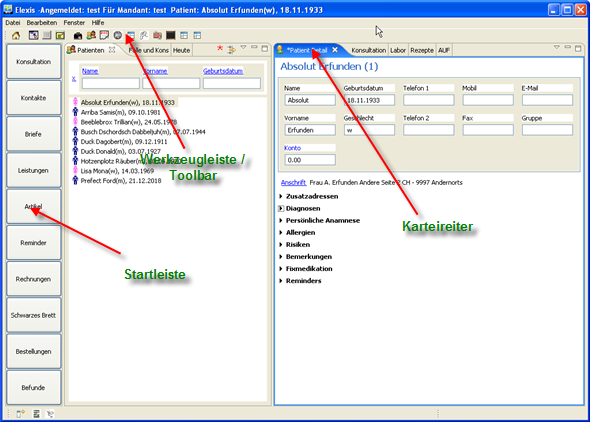
\includegraphics[width=0.8\textwidth]{images/einf0}
	\caption{Elexis Startbildschirm}
	\label{fig:startbild}
\end{figure}
\section{Patientendaten erfassen}
Aktivieren sie mit einem Klick die Ansicht 'Patienten' und schreiben Sie in die Eingabefelder Name und Vorname der neuen Patientin.
Falls die Patientin schon einmal erfasst worden ist erscheint ihr Name, in unserem Fall, wo keine Patientin dieses Namens vorhanden ist,
wird \glqq Keine Daten\grqq{}angezeigt (s. Abb. \ref{fig:patname}).
\begin{figure}[ht]
	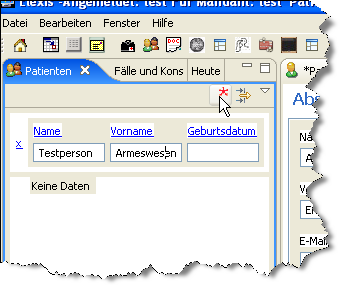
\includegraphics{images/einf1}
	\caption{Patientennamen eingeben}
	\label{fig:patname}
\end{figure}
Klicken Sie dann auf den roten Stern oben rechts, um eine Patientin mit diesen
Daten neu anzulegen. Es erscheint ein Dialogfenster (Abb. \ref{fig:patdata}), wo
Sie die Angaben in die entsprechenden Felder eingeben können.
\begin{figure}[ht]
	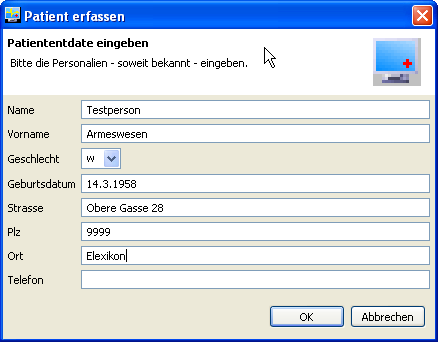
\includegraphics{images/einf2}
	\caption{Patientendaten ergänzen}
	\label{fig:patdata}
\end{figure}
Sie brauchen die hier verlangten Daten nicht vollständig einzugeben, sondern einfach soweit Sie diese im Moment kennen.
Sie müssen also im Notfalldienst nicht zuerst die vollständigen Daten eingeben, bevor Sie mit der Behandlung beginnen können.
Erfassen Sie z.B. nur Name und Geburtsdatum und überlassen Sie den Rest Ihrer MPA. Für Elexis ist ein neuer Patient in dem Moment bekannt,
wo Sie 'OK' klicken -- egal wieviele Daten zu diesem Zeitpunkt eingegeben sind.

\section{Falldaten erfassen}
Bei einer neuen Patientin müssen Sie zunächst einen \glqq Fall\grqq{} erstellen, dem
die Konsultation zugeordnet werden kann. Ein Fall sammelt alle Konsultationen, die einem gemeinsamen Garanten
zugeordnet werden können. Klicken Sie also in der \glqq Fälle\grqq{}-Ansicht
(Abb. \ref{fig:faelle1}) auf den \glqq Neu\grqq{}-Stern.
\begin{figure}[ht]
	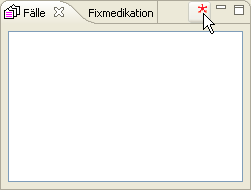
\includegraphics{images/einf3}
	\caption{Fälle-Ansicht}
	\label{fig:faelle1}
\end{figure}
Dadurch öffnet sich ein Dialog, in dem Sie wiederum die Angaben eintragen
können, soweit diese Ihnen bekannt sind (Abb. \ref{fig:falldetail})
\begin{figure}[ht]
	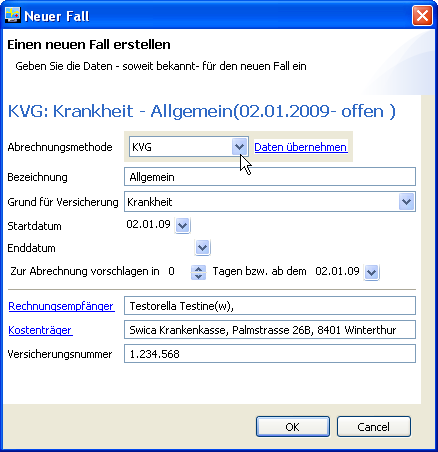
\includegraphics{images/einf4}
	\caption{Fall-Details}
	\label{fig:falldetail}
\end{figure}
Spätestens zur Rechnungsstellung müssen dann allerdings die notwendigen Angaben (Debitor, Kostenträger und Versicherungsnummer bzw. Fallnummer)
eingegeben werden.
Nach dem Klick auf OK haben Sie den neuen Fall erstellt. Bei weiteren
Konsultationen kann man sich diesen Schritt natürlich sparen.

Als nächstes erstellen wir eine neue Konsultation, wieder mit dem nun schon
bekannten Stern-Symbol (Abb. \ref{fig:neuekons}.
\begin{figure}[ht]
	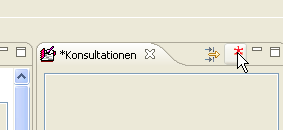
\includegraphics{images/einf5}
	\caption{Neue Konsultation}
	\label{fig:neuekons}
\end{figure}
\pagebreak[2]
Danach können wir mit dem KG-Eintrag beginnen (Abb. \ref{fig:KG}).
\section{Krankengeschichte führen}
\begin{figure}[ht]
	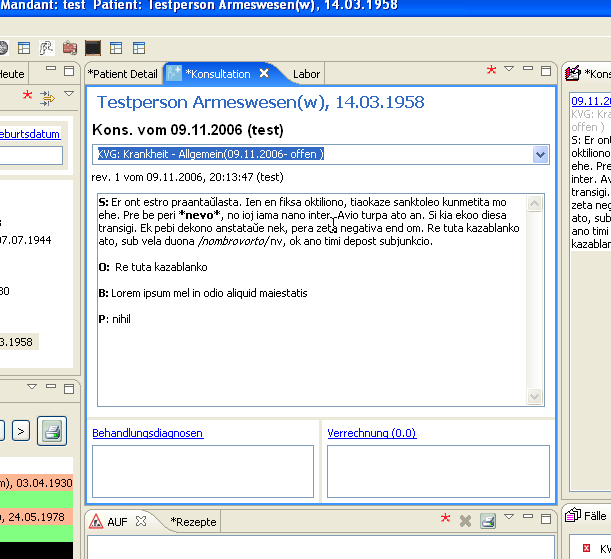
\includegraphics[width=0.7\textwidth]{images/einf6}
	\caption{KG-Eintrag}
	\label{fig:KG}
\end{figure}
Der KG-Eintrag kann einfache Textformatierungen enthalten, Textbausteine können
beliebig definiert und über eine konfigurierbare shortcut-Taste aufgerufen werden. Die Verrechnung erfolgt dann entweder über ein Tastaturmakro oder per Maus.
Nach Fertigstellung des Eintrags (auch vor oder während des Eintragens) können
Sie durch Klicken auf \glqq Verrechnung\grqq{} die Leistungen-Ansicht öffnen
(Abb. \ref{fig:Verrechnung}. Analog können sie durch klicken auf
\glqq Behandlungsdiagnosen\grqq{} die Diagnosen-Ansicht öffnen.\bigskip
\begin{figure}[ht]
	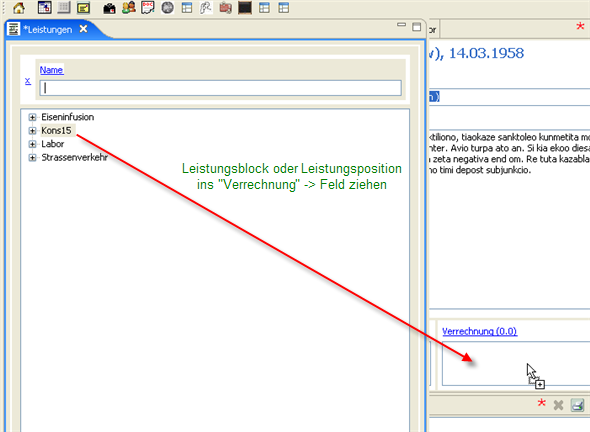
\includegraphics[width=0.7\textwidth]{images/einf7}
	\caption{Verrechnungs-Fenster}
	\label{fig:Verrechnung}
\end{figure}
Dieses Fenster enthält alle im System vorgesehenen Leistungscode-Systeme, sowie eine Seite mit selbstdefinierten Leistungsblöcken.
Sie können entweder einen ganzen Block oder einzelne Leistungen aus dem Block oder aus einem anderen Leistungsfenster (Tarmed etc.) ins \glqq Verrechnung\grqq{}-Feld ziehen (drag and drop).

Genau gleich lassen sich zur Konsultation auch Diagnosen zuordnen, auch hier hat man die Wahl zwischen allen im System integrierten Diagnosecodesystemen (beliebig anzupassen und erweiterbar).

Zum Abschluss möchten wir Ihnen noch zeigen, wie Sie eine View zur besseren Übersicht auf volle Bildgrösse und wieder
in ihren Originalzustand bringen können: Sie brauchen dazu nur auf dem Karteireiter der entsprechenden View doppelt zu
klicken (Abb. \ref{fig:viewmax}).
\begin{figure}[ht]
	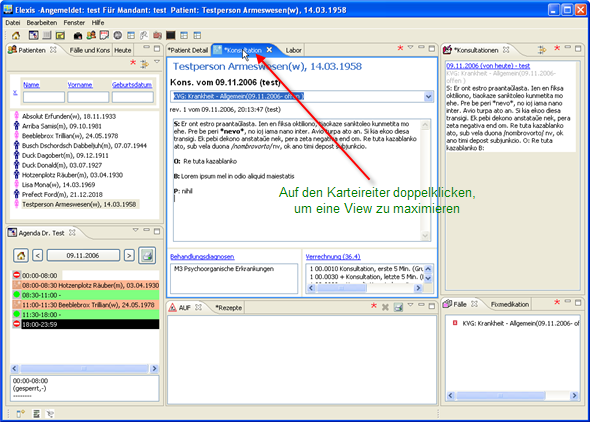
\includegraphics[width=0.9\textwidth]{images/einf8}
	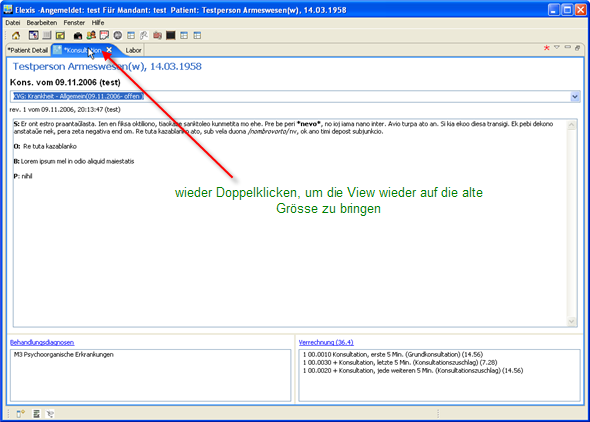
\includegraphics[width=0.9\textwidth]{images/einf9}
	\caption{View maximieren}
	\label{fig:viewmax}
\end{figure}


\chapter{Benutzeroberfläche einrichten}
	\label{customize}
	% *******************************************************************************
% * Copyright (c) 2007 by Elexis
% * All rights reserved. This document and the accompanying materials
% * are made available under the terms of the Eclipse Public License v1.0
% * which accompanies this distribution, and is available at
% * http://www.eclipse.org/legal/epl-v10.html
% *
% * Contributors:
% *    G. Weirich - initial implementation
% *
% *  $Id: customize.tex 2930 2007-07-28 16:43:29Z rgw_ch $
% *******************************************************************************
% !Mode:: "TeX:UTF-8" (encoding info for WinEdt)

\section{Funktionsprinzip}
Hervorstechendstes Merkmal vom Elexis ist die grosse Flexibilität. Wenn Sie ein anderes Praxisprogramm gewöhnt sind,
wird Ihnen die Bedienung von Elexis vielleicht etwas ungewöhnlich vorkommen. Wir möchten deshalb hier zunächst einige
grundsätzliche Konzepte erläutern.
\index{Bedienungskonzepte}
 \subsection{Schreibtisch / Perspektive}
Stellen Sie sich Ihren Arbeitstisch vor. Vermutlich werden Sie sich im Lauf der Zeit angewöhnt haben,
bestimmte Dinge an einen bestimmten Ort auf Ihrem Schreibtisch zu legen, also
Arbeitsfunktionen einem Ort zuzuordnen, wo sie sie jeweils
(idealerweise) leicht wiederfinden. Ihre Anordnung ist nicht unbedingt dieselbe wie bei jemand anderem,
der dasselbe Schreibtischmodell besitzt.

Das Programmfenster von Elexis ist so ein Schreibtisch (s. fig. \ref{fig:tour1}.Es ist in
keiner Weise festgelegt, welche Funktion
wo zu finden ist, ja es ist nicht einmal festgelegt, welche Elemente überhaupt
auf dem Schreibtisch erscheinen, und welche vielleicht irgendwo
in einer Schublade verstaut sind und nur bei Bedarf hervorgeholt werden müssen.

%\usepackage{graphics} is needed for \includegraphics
\begin{figure}[htp]
\begin{center}
  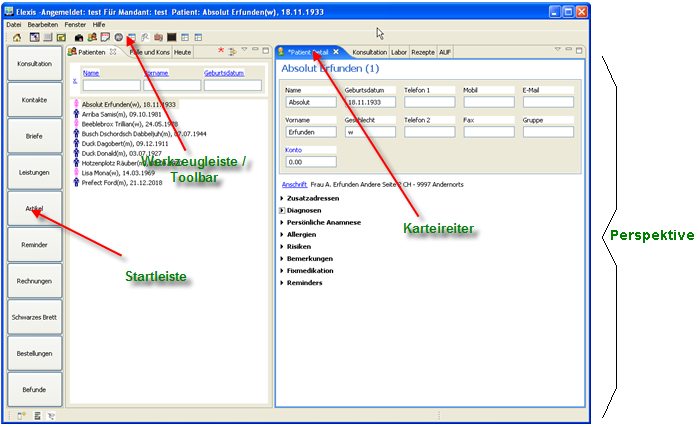
\includegraphics[width=0.9\textwidth]{images/tour1}
  \caption{Standard-Perspektive}
  \label{fig:tour1}
\end{center}
\end{figure}

Eine Anordnung von Arbeitsflächen nennen wir eine 'Perspektive' (Perspective). Die einzelnen Funktionseinheiten
(oben 'Patienten' und 'Patienten-Detail'), aus denen sich die Perspektive zusammensetzt bezeichnet
man als 'Ansicht' (View).

\subsubsection{Perspektive und Views}

Oben (fig. \ref{fig:tour1} sehen sie als Beispiel eine Perspektive, die für
einen kleinen Bildschirm geeignet ist, es zeigt einen
Screenshot auf einem 15-Zoll-TFT-Monitor. Die Ansichten \glqq
Patienten\grqq{}(links) und \glqq Patient Detail\grqq{}(rechts) liegen obenauf,
andere Ansichten sind dahinter angeordnet, so dass nur ein Karteireiter oben
zu sehen ist.
Auf einem grösseren Bildschirm würden Sie vermutlich eine andere Anordnung
bevorzugen: fig. \ref{fig:tour2} zeigt einen Screenshot auf einem
17-Zoll-TFT-Monitor mit mehreren Views gleichzeitig.

%\usepackage{graphics} is needed for \includegraphics
\begin{figure}[htp]
\begin{center}
  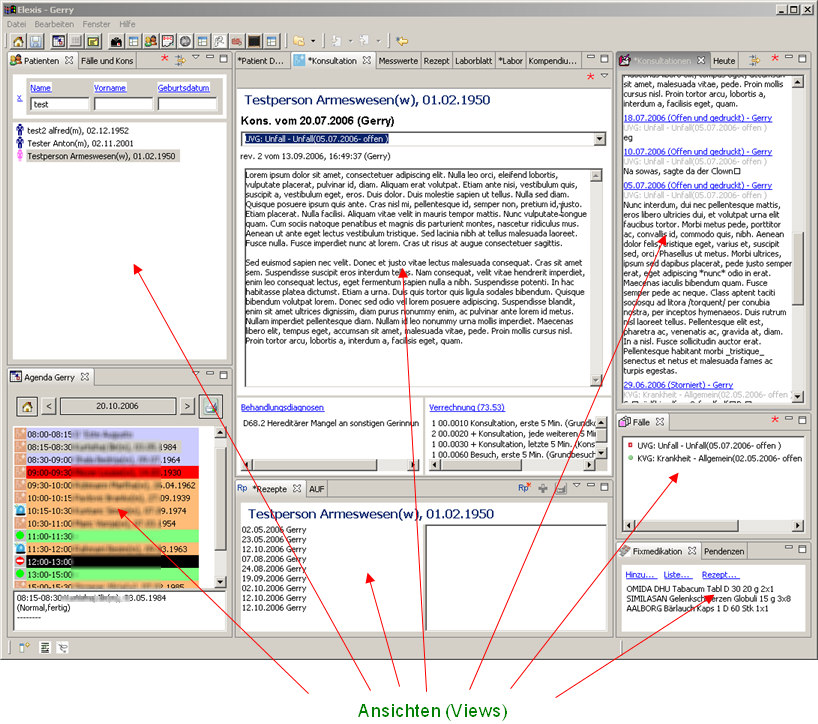
\includegraphics[width=0.9\textwidth]{images/tour2}
  \caption{Komplexere Perspektive}
  \label{fig:tour2}
\end{center}
\end{figure}
\textbf{Ansichten}

\subsubsection{Ansichten / Views}
Jede Ansicht entspricht einer bestimmten Funktionalität. Im abgebildeten Fenster sehen sie die Ansicht einer
Patientenliste (links) und die Details des 'aktiven' Patienten (rechts). Es gibt weitere Ansichten wie KG-Eintrag des aktuellen Patienten, eine Liste aller KG-Einträge, die Fixmedikation, die Rezepte,die Arbeitsunfähigkeitszeugnisse,
die Agenda etc. Jede Ansicht ist eine definierte \glqq Sicht\grqq auf die vorhandenen Daten,
daher der Name \glqq Ansicht\grqq. Sie lassen sich über die Reiter aktivieren. Die
Reiter selber lassen sich beliebig anordnen, aktivieren oder deaktivieren.

Egal wie Sie die Views angeordnet haben, jede View lässt sich zur besseren
Übersicht jederzeit auf Vollbildgrösse bringen, indem man auf den Reiter
doppelklickt (s. Abb. \ref{fig:tour3}).

\begin{figure}[htp]
\begin{center}
  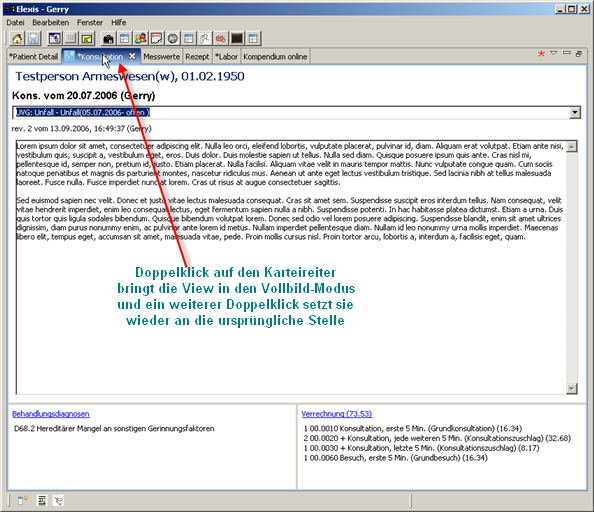
\includegraphics[width=0.9\textwidth]{images/tour3}
  \caption{View maximieren}
  \label{fig:tour3}
\end{center}
\end{figure}

\subsubsection{Views und Perspektiven anpassen}


In der Standard-Startperspektive ist links eine \glqq Startleiste\grqq{} zu
sehen. Diese führt Sie zu vordefinierten Perspektiven - es erscheinen in diesen
jeweils die passenden Ansichten. Die Werkzeugleiste führt, wie bei anderen
Programmen üblich, zu verschiedenen Funktionen. Jede Ansicht hat einen
Karteireiter, über den sie in den Vordergrund gebracht oder maximiert werden kann.

Sie können die Fensterinhalte und Ansichten völlig frei gestalten.


Die Programmfenster-Inhalte lassen sich jederzeit anpassen:
\begin{itemize}
  \item Sie können nicht benötigte Ansichten entfernen damit sie mehr Platz für
  die verbleibenden Ansichten haben
	\item können Views in der Horizontalen und Vertikalen vergrössern oder verkleinern
	\item können Views an beliebige andere Stellen des Bildschirms schieben (indem Sie sie
	an den Reitern mit gedrückter linker Maustaste \glqq festhalten\grqq{})
\end{itemize}

Jede Zusammenstellung kann als Perspektive gespeichert werden - und ist als
solche auf einfache Art wieder aufrufbar.

\subsection{Perspektiven einrichten und speichern}
Sie können nicht nur eine Perspektive erstellen, sondern beliebig viele. Ihre MPA braucht möglicherweise eine
andere Perspektive als Sie selber, z.B. wünscht sie sich die Agenda gross. Oder Sie selber verwenden unterschiedliche
Perspektiven, z.B. eine für Konsultationen und eine andere für die Buchhaltung oder wenn
Sie einen Bericht schreiben. Perspektiven lassen sich mit Elexis in wenigen Schritten zusammenstellen:\\

\bigskip

\textbf{Schritt 1: Benötigte Ansicht(en) öffnen}\\

Wählen Sie im Menu \textsc{Fenster - Ansicht - Andere}. Es öffnet sich ein Dialog wie in Abb. \ref{fig:cust1}.\\

\begin{figure}[htbp]
     \begin{minipage}{0.4\textwidth}
      \centering
       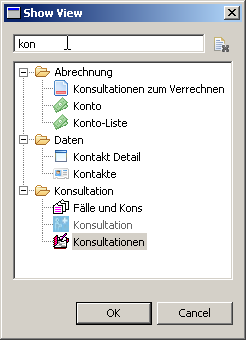
\includegraphics[width=0.8\textwidth]{images/customize1}
       \caption{View suchen}
       	\label{fig:cust1}
     \end{minipage}\hfill
     \begin{minipage}{0.5\textwidth}
        Diese Dialogbox zeigt Ihnen sämtliche Views, die in Ihrer Elexis-Installation vorhanden sind (Welche und wieviele das sind, hängt von den installierten Plugins ab). Wenn Sie in der obersten Zeile den Anfang der gesuchten View zu tippen beginnen, wird die Liste automatisch gefiltert.\\

     \end{minipage}

   \end{figure}

 \bigskip

\textbf{Schritt 2: Die Ansichten an die gewünschte Stelle schieben und auf die gewünschte Grösse bringen}

   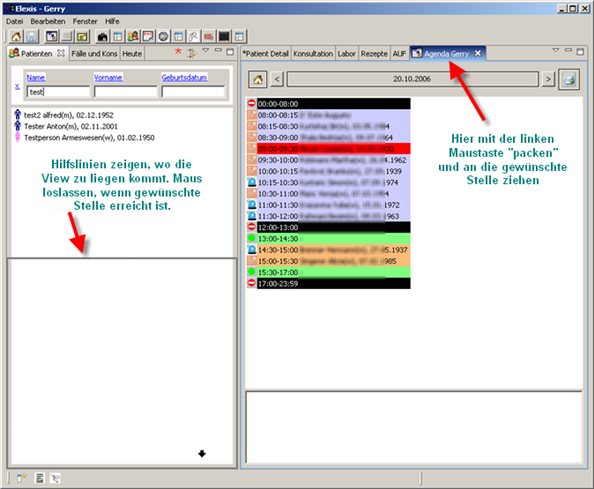
\includegraphics[width=0.8\textwidth]{images/agendagewaehlt}\\
   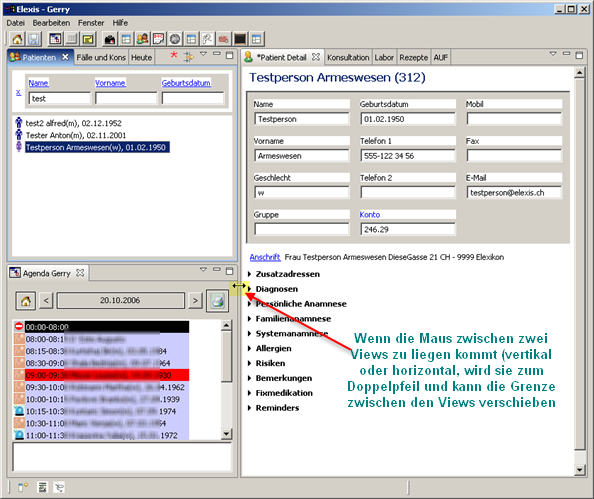
\includegraphics[width=0.8\textwidth]{images/agendaanpassen}

\bigskip
\textbf{Schritt 3:Perspektive speichern}\\
Wenn Sie möchten, dass Ihre so erstellte Perspektive auch bei späteren Programmstarts oder auf anderen Computern zur Verfügung steht, haben Sie mehrere Möglichkeiten:
\begin{itemize}
\item Wählen Sie im Menu \textsc{Fenster - Perspektive - als Startperspektive speichern}. Damit legen Sie fest, dass die eben zusammengestellte Perspektive fortan beim Anmelden erscheint.
\item \textsc{Fenster - Perspektive - speichern als...}. Damit können Sie die aktuelle Perspektive unter einem frei wählbaren Namen abspeichern. Sie können sie zu einem späteren Zeitpunkt jederzeit mit \textsc{Fenster - Perspektive - andere...} mit diesem Namen wieder zurückholen.
\item \textsc{Fenster - Perspektive - speichern}. In diesem Fall wird die aktuelle Perspektive unter ihrem bestehenden namen gespeichert.
\item Und, last but not least, Wenn Sie unter \textsc{Datei - Einstellungen - Anwender} die Perspektive unter einem bestimmten Namen speichern, dann können Sie sie auch von einer anderen Arbeitsstation aus unter diesem Namen einlesen\footnote{Dies geht allerdings natürlich nur, wenn auch auf der aufrufenden Arbeitsstation alle Views, die in dieser Perspektive definiert sind, auch vorhanden sind}. Diese Option eignet sich, um einheitliche Arbeitsumgebungen zuammenzustellen.
\end{itemize}



%%%%%%%%%%%%%%%%%%%%%%%%%%%%%%%%%%%%%%%%%%%%%%%%%%%%%%%%%%%%%%%%%%%%%%%%%%%%%%%
\part{Systematische Referenz}
\chapter{Konzepte}
	% *******************************************************************************
% * Copyright (c) 2007-2008 by Elexis
% * All rights reserved. This document and the accompanying materials
% * are made available under the terms of the Eclipse Public License v1.0
% * which accompanies this distribution, and is available at
% * http://www.eclipse.org/legal/epl-v10.html
% *
% * Contributors:
% *    G. Weirich
% *
% *  $Id: konzepte.tex 4896 2009-01-02 08:23:59Z rgw_ch $
% *******************************************************************************
% !Mode:: "TeX:UTF-8" (encoding info for WinEdt)

\section{Kontakte}
\label{kontakt}
\index{Kontakt!definition}
In Elexis ist jede Person oder Firma, die in irgendeiner Beziehung zur Praxis
steht, zunächst mal ein \glqq Kontakt\grqq{}. Kontakte werden in der
Kontakt-Perspektive eingegeben oder geändert.
\begin{flushleft}
    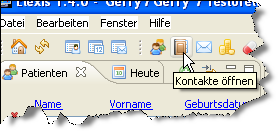
\includegraphics{images/contactperspective}
\end{flushleft}


Es gibt folgende Typen von Kontakten:
\begin{itemize}
  \item Person
	\begin{itemize}
  		\item Mandant
  		\item Anwender
  		\item Patient
  		\item Andere
    \end{itemize}
    \item{Organisation}
    \begin{itemize}
      \item{Labor}
      \item {Andere}
    \end{itemize}
\end{itemize}


\section{Anwender und Mandanten}
\index{Anwender!Definition}\index{Mandant!Definition}
Jemand, der eine Rechnungsstelle (in der Schweiz z.B. eine eigene ZSR-Nummer) hat, ist ein \textit{Mandant}. Jeder Vorgang in Elexis (Konsultation, Labor, Rezept etc.) läuft immer unter Verantwortung und auf Rechnung genau eines Mandanten. \index{Mandant}

\medskip

Jemand, der das Programm bedienen darf, ist ein \textit{Anwender}. Ein Anwender arbeitet immer im Auftrag eines bestimmten Mandanten.

Zu jedem Zeitpunkt gibt es in Elexis also einen aktuellen Mandanten und einen aktuellen Anwender.
\index{Anwender}Mandant und Anwender können auch identisch sein (Wenn der
Mandant selbst am PC arbeitet).
Ein Anwender kann auch die Mandantenzuordnung ändern (Wenn eine MPA in einer Gruppenpraxis beispielsweise für unterschiedliche
Mandantinnen arbeitet).
\index{Gruppen}\index{Rechte}
\index{Rechte}\index{Anwender!Rechte}
Anwender haben bestimmte, individuell einstellbare Rechte, mit denen man sehr
fein steuern kann, wer welche Aktionen innerhalb von Elexis steuern kann.
Anwender können auch in Gruppen zusammengefasst sein, die bestimmte gemeinsame
Rechte definieren (z.B. Gruppen \glqq MPAs\grqq{} oder \glqq Ärzte\grqq{}). Eine
spezielle Gruppe ist die Gruppe \glqq Admin\grqq{}: Wer zu dieser Gruppe gehört,
hat automatisch \textit{alle} Rechte.

\medskip

\textbf{Wichtig}: Auch wenn Ihnen das zunächst unlogisch erscheinen mag: Auch
der Chef sollte normalerweise nicht als Admin \index{Administrator} arbeiten.
Der Grund ist, dass der Admin-Account auch irreversible Löschungen und andere
sehr unangenehme Veränderungen erlaubt. Wie schnell hat man in der Hektik des
Alltags mal einen falschen Knopf geklickt!
Deswegen: Arbeiten Sie im Alltag mit einem Account, der genau diejenigen Rechte
hat, die Sie auch im Alltag brauchen. Erstellen Sie für sich einen zweiten
Account, welcher der Gruppe Admin zugeordnet ist, und melden Sie sich nur dann
unter diesem Account an, wenn es wirklich notwendig ist.

Das Konzept der Gruppen und Rechte ist ab Seite \pageref{sec:gruppen} ff.
genauer erklärt.

\section{Konsultationen, Fälle, Garanten und Kostenträger}
\index{Konsultation!Definition}\index{Fall!Definition}\index{Abrechnung}Jeder in Elexis festgehaltene Kontakt zwischen Praxispersonal und Patient ist eine \textit{Konsultation}. Wenn die Konsultation verrechnet wird, dann geht die Verrechnung zugunsten desjenigen Mandanten, für welchen der eingeloggte Anwender tätig war.
\label{definition:fall}
Jede Konsultation ist auch einem \textit{Fall} zugeordnet. Ein Fall ist hier eher eine versicherungstechnische, als eine medizinische Einheit: Der Fall sammelt alle Konsultationen, welche mit demselben Abrechnungssystem (s. \ref{settings:abrechnungssystem} auf S. \pageref{settings:abrechnungssystem}) abgerechnet werden. Dies kann manchmal identisch mit dem medizinischen Fallbegriff sein (Ein Unfall, welcher über einen bestimmten Versicherer mit einer bestimmten Fallnummer abgerechnet wird), oder er kann auch keinen Zusammenhang mit einem medizinischen Fall haben (z.B. wird in der Schweiz im Allgemeinen ein allgemeiner Fall \glqq Krankheit\grqq{} erstellt werden, der alle KVG-Konsultationen sammelt.

Ein Fall kann immer nur einen Patienten und ein Abrechnungssystem haben, kann aber durchaus  Konsultationen mehrerer Mandanten beinhalten. (Es wird dann für jeden Mandanten eine separate Rechnung erstellt).

\section{Sticker}
\index{Sticker}\index{Etiketten}\index{Markierungen}
\label{Etiketten}
Patienten und andere Datenbankinhalte können mit 'Stickern' markiert werden. Ein Sticker ist ein im Prinzip beliebiges Merkmal, das mit dem entsprechenden Datenbankobjekt verknüpft wird. Beispielsweise könnte ein Patienten mit den Stickern 'Hausarztmodell', 'MRSA' oder anderen markiert werden. Ein solcher Sticker wird beim Aufruf des entsprechenden Obekts mit angezeigt.

\textbf{Beispiele}
 Stickerwerden unter \textsc{Datei-Einstellungen-Sticker} definiert (S. Abb. \ref{fig:etiketten1}). Es können beliebig viele Sticker definiert werden. Um einen neuen Sticker anzulegen, schreiben Sie den Text für den Sticker ins obere Feld und klicken dann auf 'Neuer Sticker'. Der eben angelegte Sticker erscheint dann mit Standardwerten in der Liste. Markieren Sie ihn und geben Sie je nach Wunsch ein Bild (Format 16x16 bis höchstens 32x32 Pixel), eine Textfarbe und eine Hintergrundfarbe ein. Die Bedeutung des 'Werts' sehen Sie weiter unten.

\begin{figure}
    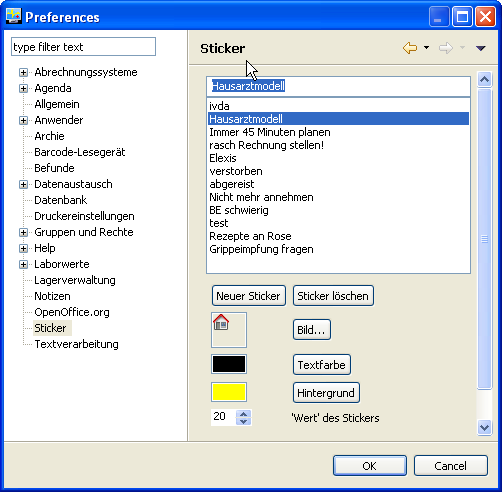
\includegraphics{images/etikette1}
    \caption{Sticker erstellen}
    \label{fig:etiketten1}
\end{figure}

So erstellte Sticker können einem Patienten durch Rechtsklick in der Patientenliste und Auswahl von 'Sticker...' zugeordnet werden. Jeder Patient kann null bis beliebig viele Sticker erhalten. In der Patientenliste wird nun der entsprechende Eintrag mit dem dem Sticker zugeordenen Bild, Vordergrund- und Hintergrundfarbe angezeigt (Abb. \ref{fig:etiketten2}).
\begin{figure}
    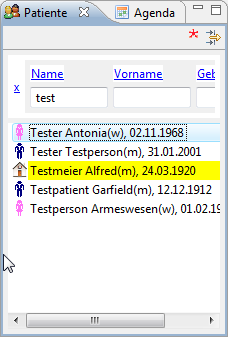
\includegraphics{images/etikette3}
    \caption{Anzeige der Sticker}
    \label{fig:etiketten2}
\end{figure}

Hier sieht man nun auch denn Sinn des 'Wert'-Attributs eines Stickers: Wenn ein Patient mehrere Sticker zugeordnet hat, dann wird in der Patientenliste immer diejenige mit dem höchsten 'Wert' angezeigt. Was für Zahlen Sie da konkret einsetzen, ist egal. Die abolute Grösse spielt keine Rolle, nur das Verhältnis zueinander.

\medskip

Wenn Sie einen Konsulaltionseintrag öffnen, sehen Sie alle zugeordneten Sticker.
\begin{figure}
    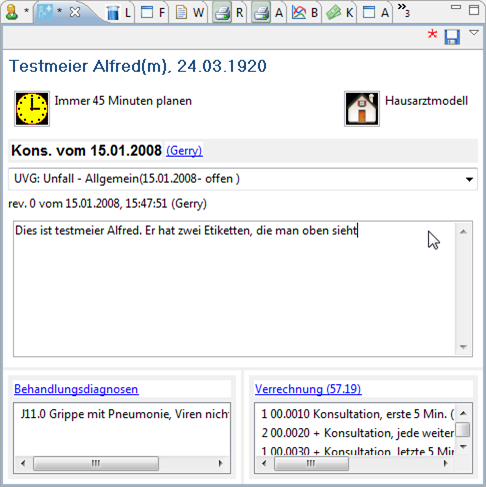
\includegraphics{images/etikette2}
    \caption{Konsultation mit Stickern}
    \label{fig:etiketten3}
\end{figure}


\clearpage

\section{Leistungsabrechnung}
\label{concept:leistung}
\index{Leistungscodes}\index{abrechnen}
\begin{wrapfigure}{l}{7.5cm}
    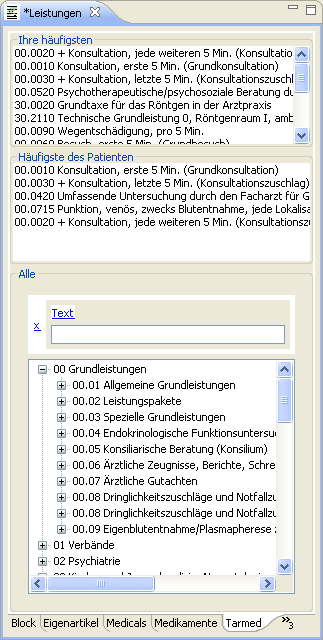
\includegraphics[width=7.5cm]{images/leistungen1}
    \caption{Leistungen}
    \label{fig:leistungen}
\end{wrapfigure}
\index{Leistungen!verrechnen}
Die Leistungscodes, die verrechnet werden können, werden einerseits von Plugins beigesteuert (z.B. Elexis-Arzttarife-Schweiz), andererseits durch von Ihnen selbst definierte Leistungsblöcke (s. weiter unten).

Alle im System vorhandenen Leistungscodesysteme sind im Fenster \glqq Leistungen\grqq{} (Abb. \ref{fig:leistungen}) untergebracht: Am unteren Rand des Fensters sehen Sie für jedes installierte Leistungscodesystem einen Reiter.

Dieses Fenster erscheint jeweils dann, wenn Sie vom Konsultationsfenster aus \glqq{}Verrechnung\grqq{} anklicken. Der Aufbau ist für jedes Leistungscodesystem gleich:

Im obersten Teilfenster stehen die von Ihnen am häufigsten angewendeten Codes dieses Leistungssystems, sind dadurch also im raschen Zugriff ohne suchen. Die Liste wird laufend aktualisiert, und je häufiger Sie einen bestimmten Code verwenden, desto weiter oben erscheint er beim nächsten Öffnen des Fensters.

\medskip
Im mittleren Teil erscheinen die bei diesem Patienten bisher am häufigsten verwendeten Codes, welche nach demselben Prinzip sortiert sind. Im untersten Teilfenster schliesslich steht das gesamte Leistungscodesystem in der vorgegebenen Systematik zur Verfügung.

\bigskip

Um einen Code zu verrechnen, können Sie ihn  aus irgendeinem der drei Abschnitte ins Verrechnung-Fenster ziehen, oder auch per Doppelklick anwählen. Manche Plugins können auch einen \glqq Optifier\grqq (Optimizer/Verifier) beinhalten, welcher Fehler erkennt bzw. Korrekturen anbringen kann. So wird etwa das Tarmed-Plugin einerseits z.B. die doppelte Verrechnung des Codes \textit{00.0010 Konsultation erste 5 Minuten} mit einer Fehlermeldung verweigern (Verifier), und andererseits wird es, wenn Sie den Code \textit{00.0030 Konsultation letzte 5 Minuten} abrechnen, automatisch auch den Code 00. 0010 dazunehmen, da 00.0030 ja immer mit 00.0010 kombiniert wird (Optimizer).
Bei \textit{Artikeln}, welche bei Direktabgabe auch von diesem Fenster aus verrechnet werden können, wird bei Verrechnung jeweils automatisch auch der Lagerbestand entsprechend nachgeführt.

\subsection{Leistungsblöcke und Eigenleistungen}
\begin{wrapfigure}{r}{6cm}
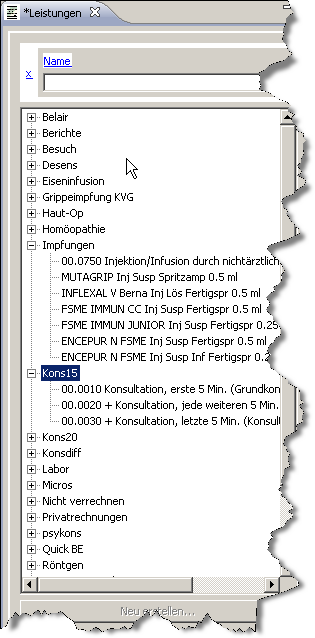
\includegraphics{images/block1}
\caption{Leistungsblöcke}
\label{fig:bloecke}
\end{wrapfigure}
\index{Leistungen!selbstdefinierte}
\index{Leistungsblock}
Als weitere Arbeitserleichterung erlaubt Elexis auch, mehrere Leistungscodes, auch aus ganz unterschiedlichen Codesystemen, zu Blöcken zusammenzufassen, die dann komplett oder teilweise verrechnet werden können. Solche Blöcke können nebst vordefinierten Leistungscodes aller installierten Codesysteme auch selbstdefinierte Elemente enthalten. In Abb. \ref{fig:bloecke} sehen Sie einige Beispiele: \textit{kons15} ist ein Beispiel für einen Block, der üblicherweise als Ganzes verrechnet wird. Dies kann man machen, indem man den Block mit der Maus ins Verrechnungs-Fenster der Konsultation zieht. Oder, falls Sie lieber mit der Tastatur arbeiten, tippt man im Konsultationstext den Namen des Blocks, gefolgt von der Makroauslösetaste (standardmässig \#). Die Eingabe von kons15\# im Konsultationstext würde also in unserem Beispiel eine 15-minütige Tarmed-Konsultation verrechnen. \textit{Impfungen} wäre ein Beispiel für einen Block, der eher als Zusammenfassung ähnlicher Elemente (als Zeitersparnis beim Heraussuchen) gedacht ist, welche meist einzeln verrechnet werden. Hier zieht man einfach die einzelnen Unterelemente aus dem Block ins Verrechnungs-Fenster.

Um einen neuen Block zu erstellen, gibt man einen (frei wählbaren, aber eindeutigen) Namen für diesen Block ein und klickt anschliessend auf \textit{Neu erstellen...}. Das Hinzufügen von Leistungen zum Block geschieht dann im Fenster Codes (s. Abb. \ref{fig:bloecke2}).
\begin{figure}[htp]
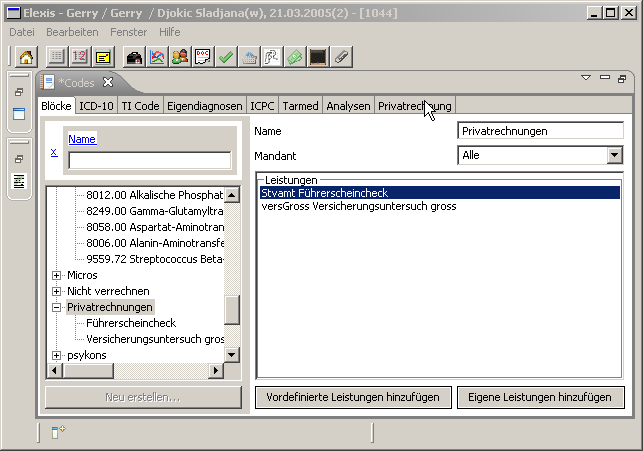
\includegraphics[width=0.9\textwidth]{images/block2}
\caption{Leistungsblock definieren}
\label{fig:bloecke2}
\end{figure}
Sie können entweder vordefinierte Leistungen aus einem der installierten Codesysteme durch drag\&drop hinzufügen, oder Sie können auch eigene Leistungen definieren. Hier müssen Sie auch Kosten und Preis in Rappen/Cents, sowie die für die Leistung budgetierte Zeit in Minuten angeben.


\section{Artikel und Lager}
\index{Artikel}\index{Medikament}\index{Lager}
 Alles was eingekauft, gelagert, abgegeben oder rezeptiert werden kann, ist ein \textit{Artikel}.
 Artikel sind in Klassen organisiert, beispielsweise \textit{Medikament},
 oder \textit{MiGeL} oder \textit{Büromaterial}.
 Elexis kann jeden Artikel, den es kennt, als \textit{Lagerartikel} aufnehmen.

 Ein Lagerartikel ist ein Artikel, dessen Bestand monitorisiert wird, und der bei Bedarf auch halbautomatisch nachbestellt werden kann.
 Weitere Informationen zu Artikeln und Lager finden Sie bei der Beschreibung der entsprechenden View (S. \pageref{view:artikel} ff.)

\section{Import von externen Daten }
\index{Import}
Elexis ist grundsätzlich in der Lage, Daten aus beliebigen Quellen zu importieren. Allerdings muss natürlich das Format dieser Daten bekannt oder in bestimmter Weise standardisiert sein. Datenimport wird deswegen meist von Importer-Plugins bewerkstelligt. Es gibt Importer für Telefunbuch-Daten, für Stammdaten anderer Praxisprogramme, für externe Labors, für Laborgeräte und für andere medizinische Geräte, die ihre Daten zu einem Computer transferieren können, für MiGeL, Medikamente, Tarmed und andere Datenbanken usw. Eine Aufstellung erhältlicher Plugins finden Sie im Menu 'Plugins' auf http://www.elexis.ch. Zusätzliche Importer können meist relativ einfach programmiert werden, verlangen Sie ggf. einen Kostenvoranschlag.

\medskip

Importer befinden sich meist im lokalen Menü der View, die die entsprechenden Daten anzeigt (z.B. Tarmed-Importer oder Labor-Importer). Eine Klasse von Importern, die keiner bestimmten View zugeordnet sind, hängen sich auch im Datei-Datenimport-Menü ein. Hier öffnet sich ein Dialog wie in Abb. \ref{fig:importdlg}.
\begin{figure}
  % Requires \usepackage{graphicx}
  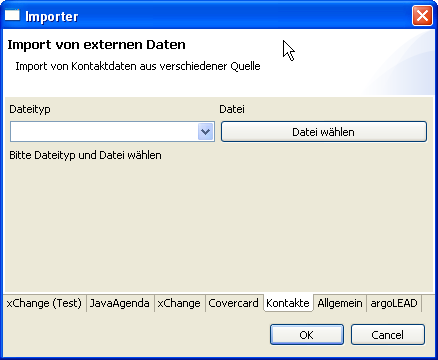
\includegraphics{images/importdlg}\\
  \caption{Import-Dialog}\label{fig:importdlg}
\end{figure}
\index{Import!Kontakte}
In den Reitern unten finden Sie alle installierten allgemeinen Importer. Welche das sind, hängt von den vorhandenen Plugins ab. Lediglich der in der Abbildung in den Vordergrund gebrachte 'Kontakt-Importer' ist immer vorhanden. Dieser Importer kann Kontakte aus externen Dateien importieren, sofern diese auf eine standardisierte Weise als Tabellen aufbereitet sind. Wählen Sie unter 'Dateityp', ob es sich um eine Microsoft\texttrademark Excel\texttrademark Tabelle (xls), um eine Character Separated Values-Tabelle (csv)oder um die Santésuisse-Tabelle der Versicherer und ihrer EAN-Codes handelt.
Im Fall von xls muss die Datei eine Tabelle 0 mit folgenden Spalten enthalten:
\begin{tabular}[h]{|l|l|}
\hline Spaltentitel & Erklärung\\
\hline
\hline  ID & eine (im Prinzip beliebige, innerhalb der Datei aber eindeutige) Identifikation\\
\hline IstPerson & 1 wenn der Eintrag eine Person bezeichnet, 0 andernfalls (Organisation etc.)\\
\hline Titel & Ein Titel, Anredem Bezugsperson etc.\\
\hline Bezeichnung1 & Bei Personen der Name\\
\hline Bezeichnung2 & Bei Personen der Vorname\\
\hline Zusatz & \\
\hline Geburtsdatum & Im Format dd.mm.yyyy oder yyyy-mm-dd\\
\hline Geschlecht & m oder f oder w oder ein Wort, das mit m oder f oder w anfängt.\\
\hline E-Mail & die E-Mail-Adresse\\
\hline Website & Eine WWW-Adresse\\
\hline Telefon 1 & Primäres Telefon\\
\hline Telefon 2 & weitere Nummer\\
\hline Mobil & Mobiltelefon\\
\hline Strasse & Strasse und Hausnr.\\
\hline Plz & PLZ entweder als 1224 oder CH-1224 geschrieben\\
\hline Ort & \\
\hline Postadresse & Adresse, wie sie auf Adressetiketten erscheinen soll. Zeilensprünge als $\backslash$n\\
\hline EAN & Die EAN als EAN13\\
\hline
\end{tabular}

\medskip

Die erste Zeile der Tabelle muss die Spaltentitel genau in obiger Schreibweise enthalten, damit das Format erkannt werden kann.
Jede der genannten Spalten muss vorhanden sein, darf aber leer sein. Die Datei muss als iso-8859-1 codiert sein (Das ist Standard unter Windows; bei der MAc-Version von Excel müsste die Exportcodierung ev. entsprechend angepasst werden).

\medskip

Wenn Sie den Dateityp festgelegt haben, Klicken Sie auf den Button 'Datei wählen' und suchen die entsprechende Importdatei auf. Setzen Sie ein Häkchen bei 'ID beibehalten' \textbf{nur dann}, wenn \begin{itemize}
\item Jeder Datensatz im Feld ID eine ID hat
\item Diese ID garantiert eindeutig ist, also mit keinem anderen Kontakt in Elexis kollidieren kann
\item Sie diese ID unbedingt beibehalten wollen
\end{itemize}
Wenn Sie das Häkchen nicht setzen, was in den meisten Fällen empfohlen ist, dann wird Elexis beim Import für jeden Kontakt eine eigene eindeutige ID erstellen (genauso, als würde man den Kontakt manuell neu anlegen).\\
Klicken Sie dann OK, um den Import zu starten.

 \section{Mehrere Instanzen gleichzeitig}
 \index{gleichzeitig}
 Sie können Elexis problemlos mehrfach starten und dann in verschiedenen
 Fenstern unterschiedliche Perspektiven oder verschiedene Patienten anzeigen.
 Einzelne Elemente können auch mit Cut\&Paste zwischen den laufenden Instanzen
 ausgetauscht werden.
 Anwendungsbeispiele:
 \begin{itemize}
   \item Sie arbeiten an einem Patienteneintrag und es kommt ein Telefon
   betreffend eines anderen Patienten. Anstatt Ihre Arbeit zu verlassen, bringen
   Sie die zweite Elexis-Instanz in den Vordergrund und suchen dort den neuen
   Patienten auf.
   \item Die MPA möchte an ihrem Arbeitsplatz Agenda und Patientendaten
   gleichzeitig im Blick haben. Spendieren Sie ihr einen zweiten Monitor (statt
   eines zweiten PC's), schliessen Sie beide Monitore an einer DualHead-fähigen
   Grafikkarte am selben PC an und schieben Sie in jeden Monitor eine eigene
   Instanz von Elexis.
   \item Während Elexis mit einem langwierigen Rechnungsdruck beschäftigt ist,
   möch\-ten Sie nicht untätig herumsitzen. Kein Problem, starten Sie eine zweite
   Instanz von Elexis und arbeiten Sie dort weiter. (Sie könnten natürlich auch
   einen Kaffee trinken oder einen Spaziergang machen).
   \item Sie erstellen einen Brief, möchten aber einzelne Stellen aus einem
   anderen Brief herüberkopieren. Laden Sie in der einen Elexis-Instanz den
   alten Brief, erstellen Sie in der anderen den neuen Brief und kopieren Sie
   das gewünschte mit Cut\&Paste.
 \end{itemize}

\section{Plugins}
\index{Plugin!Definition}
Dieses Konzept wird auf Seite \pageref{expl:plugins} genauer besprochen. Hier nur soviel: Elexis ist nach allen Seiten frei erweiterbar. Es gibt nicht nur eine vorgegebene Zahl von \glqq Modulen\grqq{}, sondern tatsächlich können jederzeit auch von Dritten neue Funktionen programmiert werden, von denen zum Zeitpunkt des Programmreleases noch gar nichts bekannt war. Dies geschieht in Form von sogenannten \glqq Plugins\grqq{}. Plugins können beispielsweise für Statistik, Buchhaltung, Import von Labordaten, Anbindung von Apparaten, Export von KG-Daten, neue Abrechnungssysteme, neue Diagnosesysteme usw. programmiert werden.

Ein Elexis-Plugin ist also einfach ein Programm mit im Prinzip beliebigen Fähigkeiten, welches die Eigenschaft hat, mit Elexis zusammenarbeiten zu können.

Es kann weder in diesem Handbuch noch sonstwo eine abschliessende Aufzählung aller Plugins geben, weil niemand wissen kann, welche Plugins von unabhängigen Anwendern bei unabhängigen Programmierern in Auftrag gegeben worden sind. 
\chapter{Menü und Toolbar} 					
	% *******************************************************************************
% * Copyright (c) 2007 by Elexis
% * All rights reserved. This document and the accompanying materials
% * are made available under the terms of the Eclipse Public License v1.0
% * which accompanies this distribution, and is available at
% * http://www.eclipse.org/legal/epl-v10.html
% *
% * Contributors:
% *    G. Weirich - initial implementation
% *
% *  $Id: menu.tex 4903 2009-01-03 11:44:22Z rgw_ch $
% *******************************************************************************
% !Mode:: "TeX:UTF-8" (encoding info for WinEdt)

% Dieses Dokument enthält die Dokumentation der Menübefehle

\section{Menu}
Le menu est - comme la plupart des éléments d'Elexis- pas fixe. Les Plugins peuvent ajouter des propres commandes de menu ou des sous-menus entiers. Ce qui suit ne décrit par conséquent que le contenu des menus qui existent dans l'installation de base de Elexis.

\begin{itemize}
  \item {\textsc{fichier -- utilisateur}: S'annoncer comme autre utilisateur. Une boîte de dialogue s'ouvre dans laquelle on introduit le nom de l'utilisateur et un mot de passe.
Lorsqu'on clique sur  \glqq abandonner\grqq{}on clôture seulement la session de sorte qu'il n'y ait plus d'utilisateur branché. Il est recommandé d'installer pour chaque utilisateur son propre compte puisque Elexis lie la plupart des actions à un nom d'utilisateur, et puisque les droits d'utilisateur dépendent également de l'utilisateur connecté.}
  \item {\textsc{fichier -- mandant}: Activer un autre mandant. Dans ce cas, l'utilisateur actuel reste le même, toutefois il travaille pour un autre mandant. Cela signifie entre autres que le décompte des prestations de même que la responsabilité médicale en définitive vont sur le compte de ce mandant. Il est ainsi essentiel que dans un cabinet de groupe le mandant correct soit toujours activé. Elexis indique dans l'entête le nom de l'utilisateur actuel et le nom du Mandant actuel respectivement.}
  \item {\textsc{fichier -- connexion}: Etablir et/ou. modifier la connexion à la base de données.
Ceci n'est important que lors de l'installation du programme et peut être lu sous la rubrique concernant l'installation.}
  \item {\textsc{fichier -- Options}: Configuration centrale. La description en détail se trouve sous 'Configuration'.  (voir page \pageref{settings} et suivantes).}
  \item {\textsc{fichier -- Importation de données }: Ici, des données étrangères de différent type peuvent être importées (données de contact, données d'autres logiciels de gestion du cabinet etc.). Les options disponibles dépendent de installation des Plugins d'importation} \footnote{Il existe p.ex. un 'Plugin' d'importation pour le logiciel \textit{Aeskulap}. Un autre Plugin existe pour \textit{PraxisStar}. Informations et achat par l'intermédiaire du support (ad) elexis.ch}
  \item {\textsc{fichier -- fermer}: Fermeture du programme}
  \item {Le menue \glqq Edition\grqq{} est prévu comme dans d'autres programmes pour le presse-papiers.}
  \item {\textsc{fenêtre -- fixer perspective }: Cela sert à protéger la perspective actuelle des modifications par erreur. Des perspectives essentiels ne peuvent pas être fermés tant que se trouve un crochet devant ce point de menu.}
  \item {\textsc{fenêtre -- perspective -- enregistrer perspective }: Par ceci, vous sauvegardez l'aménagement des affichages actuels sous le même nom de perspective qu'elle a eu avant.}
  \item {\textsc{fenêtre -- perspective -- enregistrer perspective sous \ldots}:
  Par ceci, vous sauvegardez l'aménagement des affichages actuels sous un nouveau nom de perspective.}
  \item {\textsc{fenêtre -- perspective -- annuler perspective }: Reconduit la perspective actuelle à l'aménagement des affichages qu'elle avait avant la dernière sauvegarde. Peut rétrograder toutes les dernières modifications.}
  \item {\textsc{fenêtre -- perspective -- sauvegarder comme perspective de démarrage }: Déclare la perspective actuelle comme perspective de démarrage pour l'utilisateur actuel. Ainsi cette perspective apparaît après le login de l'utilisateur actuel.}
  \item {\textsc{fenêtre -- perspective -- autre }: Une boîte de dialogue, avec laquelle vous pouvez faire apparaître touts les affichages/Views existants dans le système classifiés d'après les thèmes. Vous pouvez feuilleter la liste ou introduire le nom de l'affichage recherché dans la case prévue.}
  \item {\textsc{denêtre - affichage }: Dans ce menu, on énumère d'abord quelques affichages (Views) qui font partie des perspectives standard. Cliquez sur un titre pour ouvrir l'affichage en question.}
  \item {\textsc{fenêtre - affichage - autre }: Il apparaît une boite de dialogue dans laquelle vous pouvez accéder, groupées par thème, à toutes les 'Views' existantes dans le système. Vous pouvez feuilleter la liste ou taper le nom de la 'View' dans la case prévue pour cela.}
\end{itemize}

\section{Barre d'outils}
La barre d'outils qui se trouve au-dessous du menu est également configurable par des Plugins ou par vos réglages personnels. Elle met à disposition des fonctions pour accéder aux perspectives (voir page \ref{perspektiven})
et pour imprimer des étiquettes. Si vous passez simplement avec la souris sur un bouton et si vous attendez un petit moment, la fonction du bouton en question est indiquée comme texte. 
\chapter{Views des Kernsystems}
	% *******************************************************************************
% * Copyright (c) 2007 by Elexis
% * All rights reserved. This document and the accompanying materials
% * are made available under the terms of the Eclipse Public License v1.0
% * which accompanies this distribution, and is available at
% * http://www.eclipse.org/legal/epl-v10.html
% *
% *  $Id: einfuehrung.tex 4904 2009-01-03 17:58:33Z rgw_ch $
%
%*******************************************************************************
% !Mode:: "TeX:UTF-8" (encoding info for WinEdt)

\section{Einleitung}
Views (Ansichten) sind die zentralen Anzeige- und Bedienungselemente in Elexis.
Eine View zeigt eine bestimmte Art von Daten in einer bestimmten Weise an und
kann definierte Bearbeitungen dieser Daten ermöglichen. Diese Views können Sie
je nach Bedürfnissen und Arbeitsgewohnheiten selbst zu sogenannten Perspektiven
zusammenstellen und abspeichern. Man auch an verschiedenen Arbeitsplätzen
verschiedene Perspektiven einrichten, da ja beispielsweise am Empfang, im Labor
und im Arztzimmer unterschiedliche Arbeiten im Vordergrund stehen.

Im Gegensatz zu anderen Praxisprogrammen wird bei Elexis die Benutzeroberfläche
also nicht vom Hersteller, sondern vom Anwender des Programms definiert.

In diesem Kapitel werden diejenigen Views beschrieben, die im Grundsystem von
Elexis eingeschlossen sind. Eine solche Aufzählung kann nie abschliessend sein,
da (von uns oder anderen) neu entwickelte Plugins jederzeit eigene Views
mitbringen können. Diese müssten dann in der Dokumentation des betreffenden
Plugins beschrieben sein.

\subsection{Öffnen und Schliessen einer View}
Alle im System vorhandenen Views (auch die, die von externen Plugins mitgebracht
werden) sind unter dem Menüpunkt \textsc{Fenster-Ansicht} erreichbar. In diesem
Menü finden sich manchmal einige Views, die für die aktuelle Perspektive
zusammengestellt wurden, sowie immer ein Menüpunkt \glqq Andere\ldots\grqq{}
resp. \glqq Other\ldots\grqq{}. Hier ist eine nach Themen gruppierte Liste aller
Views zu finden (s. Abb. \ref{fig:viewlist}).
%\usepackage{graphics} is needed for \includegraphics
\begin{figure}[htp]
\begin{center}
  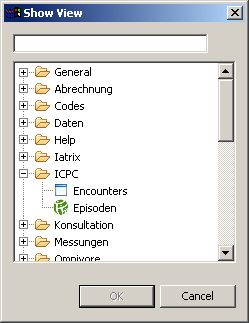
\includegraphics{images/showviewdialog}
  \caption{Liste aller Views}
  \label{fig:viewlist}
\end{center}
\end{figure}

Sie können entweder diese Liste durchblättern, oder Sie können den Namen der
gesuchten View im Textfeld oben eintippen. Sobald Sie anfangen zu tippen, wird
die Liste sofort auf die zu den getippten Buchstaben passenden Einträge
gefiltert.

Markieren Sie dann die gewünschte View und öffnen Sie sie entweder durch
Doppelklick oder Klick auf \glqq OK\grqq{}.

\par
Um eine View zu schliessen genügt es, auf das  X- Symbol im Karteireiter der
betreffenden View zu klicken.

\subsection{Öffnen und Speichern einer Perspektive}
\label{perspektiven} \index{Perspektive}
Eine Perspektive ist wie oben gesagt eine benannte Zusammenstellung von Views.
Elexis bringt einige vordefinierte Perspektiven mit, welche über die Startleiste
resp. die Toolbar aufgerufen werden können. (Vgl auch Abb. \ref{fig:toolbar}).

Eine Perspektive hat als \glqq Startperspektive\grqq{} eine spezielle Bedeutung:
Diese Perspektive wird immer automatisch nach dem Einloggen des entsprechenden
Anwenders auf dem betreffenden Arbeitsplatz eingestellt, sowie nach Klick auf das
'Home'-Symbol (der Button ganz links auf der Toolbar). Alle anderen (beliebig
viele) Perspektiven können unter einem frei wählbaren Namen abgespeichert und
wieder aufgerufen werden. Perspektiven sind Arbeitsplatz-Spezifisch (Eine auf
einem Arbeitsplatz eingestellte Perspektive steht also nicht automatisch auf
anderen Arbeitsplätzen zur Verfügung)\footnote{Dies muss so sein, da ja auch
nicht auf allen Arbeitsplätzen dieselben Plugins zur Verfügung stehen müssen -
vielleicht muss Ihr Buchhaltungs-Plugin nicht unbedingt auch auf dem Labor-PC
aktiv sein.}.

\begin{itemize}
\index{Perspektive!Startperspektive}
\item Um die aktuell eingestellte View-Anordnung als Startperspektive zu
speichern,
wählen Sie den Menüpunkt \textsc{Fenster -- Perspektive -- als Startperspektive
speichern}.

\item Um die aktuelle Perspektive neu (z.B. mit veränderter Viewanordnung oder
-Grösse) zu speichern, wählen Sie das Menü \textsc{Fenster -- Perspektive --
Speichere Perspektive}.

\item Um die aktuelle View-Anordnung unter einem eigenen Perspektivennamen
zu speichern, wählen Sie das  Menü \textsc{Fenster -- Perspektive -- Speichere Perspektive als\ldots}

\item Um die aktuelle Perspektive wiederherzustellen (falls Ihnen die gemachten
Ver\-än\-de\-run\-gen nicht zusagen, oder falls Sie versehentlich Views geschlossen
haben), wählen Sie \textsc{Fenster -- Perspektive -- Wiederherstellen}

\item Um zur Startperspektive zurückzukehren, klicken Sie auf das Haus-Symbol
ganz links in der Toolbar
\item Um eine früher gespeicherte Perspektive aufzurufen, wählen Sie
\textsc{Fenster -- Perspektive -- Andere} und wählen die gewünschte Perspektive
aus der Liste aus.

\end{itemize}

	% *******************************************************************************
% * Copyright (c) 2007 by Elexis
% * All rights reserved. This document and the accompanying materials
% * are made available under the terms of the Eclipse Public License v1.0
% * which accompanies this distribution, and is available at
% * http://www.eclipse.org/legal/epl-v10.html
% *
% * Contributors:
% *    G. Weirich - initial implementation
% *
% *  $Id: stammdaten.tex 2472 2007-06-03 09:48:14Z rgw_ch $
% *******************************************************************************
% !Mode:: "TeX:UTF-8" (encoding info for WinEdt)

\section{Stammdaten-Views}

\subsection{Patienten}
Die Patientenliste dient sowohl der Anzeige existierender Patienteneinträge, als
auch dem Erfassen neuer Einträge. Die Liste zeigt all diejenigen Kontakte an,
die als Patient markiert sind.
\begin{figure}[ht]
	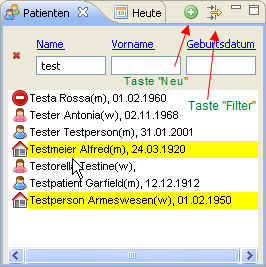
\includegraphics{images/patlistview}
	\caption{Patientenliste}
	\label{fig:patlist}
\end{figure}
Die Eingabefelder oben (Name, Vorname, Geburtsdatum) dienen dem Filtern der
Liste gemäss den gewünschten Parametern.
\begin{itemize}
  \item Bei Name und Vorname gilt:
	\begin{itemize}
      \item Wenn Sie mindestens zwei Buchstaben eingeben, erscheinen in der
      Liste nur noch diejenigen Einträge, die mit diesen Buchstaben \textit{beginnen}.
      \item Wenn Sie das Zeichen \% und mindestens zwei weitere Buchstaben
      eingeben, dann erscheinen in der Liste diejenigen Einträge, die diese
      Zeichenfolge \textit{enthalten}.
    \end{itemize}
  \item Beim Geburtsdatum gilt:
	\begin{itemize}
      \item Wenn Sie mindestens 3 aufeinanderfolgende Ziffern eingeben, dann wird
      die Zahl als Jahreszahl interpretiert und es werden diejenigen Patienten
      ausgewählt, die das entsprechende \textit{Geburtsjahr} haben.
      \item Wenn Sie zwei Ziffern, gefolgt von einem Punkt und ggf. weitere 2
      Ziffern eingeben, dann werden diejenigen Patienten angezeigt, die den
      entsprechenden \textit{Geburtstag} und ggf. \textit{Geburtsmonat} haben.
      Beachten Sie bitte, dass Sie Tag und Monat zweistellig eingeben müssen,
      also z.B. 04.05. und nicht etwa 4.5.
     \end{itemize}
\end{itemize}
Wenn keine Einträge existieren, die den eingegebenen Filterbedingungen
entsprechen, dann wird in der Liste angezeigt: \glqq keine Daten\grqq.
\subsubsection{Toolbar}
\begin{itemize}
  \item Mit der Taste \glqq Neu\grqq{} (s. Abb. \ref{fig:patlist}) können Sie
  einen neuen Patienten erfassen. Klick
  auf diesen Knopf öffnet die Patienteneingabe-Dialogbox. Diejenigen Felder, die
  Sie bereits eingegeben haben, sind vorgegeben, die anderen können Sie soweit
  eingeben, wie sie im Moment bekannt sind. Mit Klick auf \glqq OK\grqq{}wird
  der neue Patienteneintrag angelegt. Bei Klick auf \glqq Abbrechen\grqq{}werden
  die eingegebenen Daten verworfen und es wird kein neuer Eintrag erstellt.
  Falls ein neuer Eintrag erstellt werden soll, und bereits ein Eintrag mit
  gleichen Daten existiert, dann erfolgt eine Rückfrage.

  \item Mit der Taste \glqq Filter\grqq{} (s. Abb. \ref{fig:patlist}) können Sie
  die Liste nach
  verschiedenen Kriterien filtern (s. Abb. \ref{fig:patlistfilter}).
	\begin{figure}[ht]
    	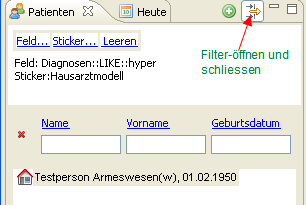
\includegraphics{images/patlistfilter}
    	\caption{Filterbedingungen eingeben}
    	\label{fig:patlistfilter}
    \end{figure}
	\textbf{Achtung}: Der Filter rastet ein und wird erst wieder aufgehoben, wenn
	Sie erneut auf den Filter-Knopf klicken. Solange er eingerastet ist, wirken
	alle anderen Eingaben nur auf die bereits gefilterte Auswahl.
\end{itemize}
\subsubsection{View-Menü}
Das lokale Menü (s. Abb. \ref{fig:patlist}) enthält folgende Einträge:
\begin{itemize}
  \item Patient löschen (sofern der angemeldete Anwender die hierfür notwendigen
  Rechte hat): Damit kann ein Patienteneintrag definitiv und unwiderruflich aus
  der Datenbank gelöscht werden. Dies ist nur dann möglich, wenn zu diesem
  Patienten keine Fälle (mehr) existieren.
  \item Liste filtern: Dies öffnet ebenfalls die Filter-Dialogbox (s.o.)
\end{itemize}

\subsubsection{Kontextmenü}
Das Kontextmenü erscheint, wenn Sie auf einem Pa\-tien\-ten\-eintrag mit der rech\-ten
Maus\-taste klicken. Es enthält fol\-gende Ein\-träge:
\begin{itemize}
  \item Patient löschen (s. oben)
  \item KG exportieren. Falls ein Export-Plugin installiert ist, wird die KG des
  aktuell markierten Patienten über dieses Plugin exportiert. Falls mehrere
  Export-Plugins definiert sind, erscheint zunächst eine Dialogbox, mit der sie
  das gewünschte Ziel bzw. Format auswählen können.
\end{itemize}


\subsection{Patient-Detail}
Diese View (Abb. \ref{fig:patdetail} zeigt Details des momentan ausgewählten
Patienten resp. der momentan ausgewählten Patientin an
 %\usepackage{graphics} is needed for \includegraphics
\begin{figure}[htp]
\begin{center}
  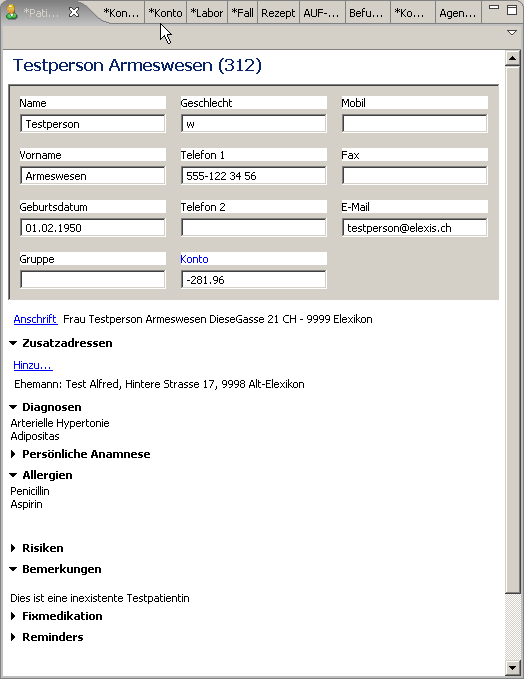
\includegraphics[width=0.9\textwidth]{images/patdetail}
  \caption{Patient Detailansicht}
  \label{fig:patdetail}
\end{center}
\end{figure}
Alle Felder können durch einfaches Überschreiben geändert werden, sofern der
aktuell eingeloggte Anwender die dazu erforderlichen Rechte besitzt. Eine
Änderung wird in dem Moment gespeichert, in dem ein Feld wieder verlassen wird.
(Explizites Speichern ist in Elexis nie notwendig).

Die Felder im oberen Block sind alle einzeilige Textfelder und können direkt geändert
werden, bis auf das Feld \glqq Konto\grqq{}, welches nicht direkt beschreibbar
ist. Dieses Feld stellt den Saldo aller Forderungen an diesen bzw. Zahlungen von
diesem Patienten dar. Wenn der aktuell eingeloggte Anwender Verrechnungs-Rechte
besitzt, kann er den blauen Text \glqq Konto\grqq{} anklicken, dann öffnet sich
ein Dialog, in dem einzelne Buchungen eingegeben werden können.

\textbf{Achtung}: Normalerweise erfolgen Buchungen automatisch durch Erstellen
von Rechnungen und Einlesen von ESR-Files. Manuelle Buchungen können zu
Inkonsistenzen in der Buchhaltung führen. Führen Sie also nur dann manuelle
Buchungen durch, wenn Sie sich über die Konsequenzen exakt bewusst sind.

Das Feld \glqq Anschrift\grqq{} zeigt die Postanschrift des Patienten an. Diese
kann durch Klick auf den blauen Text \glqq Anschrift \grqq{}geändert werden.

Die darunterstehenden Felder sind alle aufklappbar: Standardmässig ist nur der
Titel sichtbar, durch Klick darauf öffnet sich das Feld.
\begin{itemize}
  \item Das Feld \glqq Zusatzadressen\grqq{}dient dazu, Kontakte, die in
  irgendeiner Beziehung zum Patienten stehen, zu erfassen. Beispielsweise
  Angehörige, Ämter, weitere Ärzte etc. Klick auf \glqq Hinzu\grqq{} öffnet eine
  Kontaktauswahl-Box, aus der die gewünschte Person oder Organisation ausgewählt
  werden kann. Danach erscheint eine Eingabebox, in der die Beziehung des eben
  ausgewählten Kontakts zum Patienten beschrieben werden kann. \\
  Mit Rechtsklick auf einen Eintrag in diesem Feld öffnet sich ein Kontextmenü,
  mit dem man den vollständigen Eintrag anzeigen, oder den Eintrag entfernen kann.
  \item Die Felder \glqq Diagnose\grqq, \glqq Persönliche Anamnese\grqq{},
  \glqq Allergien\grqq{}, \glqq Risiken\grqq{} und \glqq Bemerkungen\grqq{}
  können direkt beschrieben werden und werden wie gewohnt sofort beim Verlassen
  gespeichert.
  \item Das Feld \glqq Fixmedikation\grqq{}entspricht der View Fixmedikation.
  \item Das Feld \glqq Reminders\grqq{} zeigt die Reminders zum aktuellen Patienten.
\end{itemize}
\subsection{Kontakte}
Diese View (Abb. \ref{fig:kontaktlist}) zeigt eine Liste aller in Elexis
vorhandenen Kontakte an. Ein Kontakt
ist jede Person oder jede Organisation, welche in irgendeiner Beziehung zu
unserer Praxis steht. Das sind beispielsweise Patienten, Kollegen, Spitäler,
Versicherungen, Labors, Lieferanten usw.
%\usepackage{graphics} is needed for \includegraphics
\begin{figure}[htp]
\begin{center}
  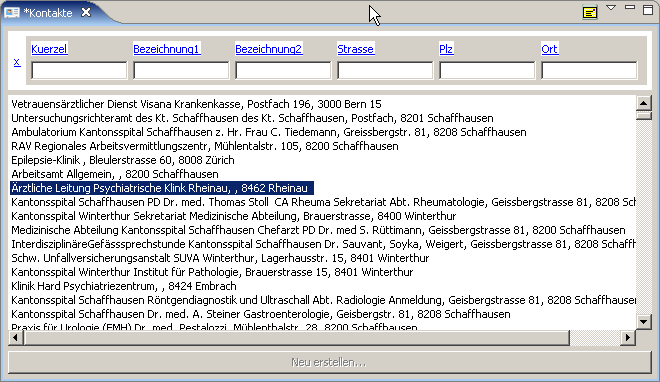
\includegraphics[width=0.9\textwidth]{images/kontaktlistview}
  \caption{Kontaktliste-View}
  \label{fig:kontaktlist}
\end{center}
\end{figure}
Mit Klick auf das Briefumschlag-Symbol rechts oben können Sie eine
Adressetikette für den betreffenden Kontakt ausdrucken.

\subsection{Kontakt-Detail}
Hier werden die Details zum aktuell ausgewählten Kontakt angezeigt und können
geändert werden (Abb. \ref{fig:kontaktdetail}).
%\usepackage{graphics} is needed for \includegraphics
\begin{figure}[htp]
\begin{center}
  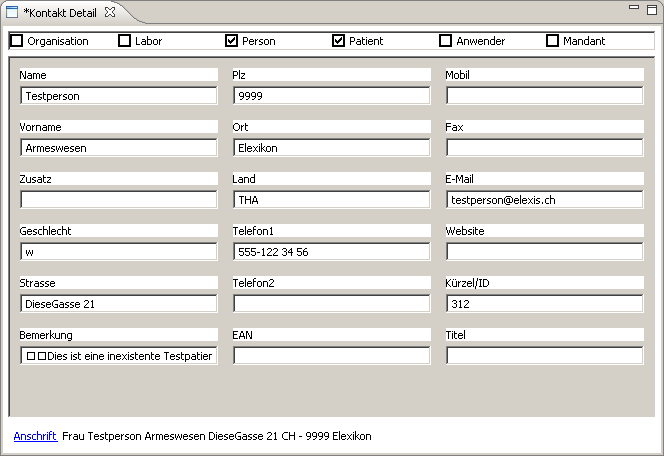
\includegraphics[width=0.9\textwidth]{images/kontaktdetail}
  \caption{Kontakt Detailview}
  \label{fig:kontaktdetail}
\end{center}
\end{figure}
In den Checkboxen der obersten Zeile können Sie den Typ des betreffenden
Kontakts festlegen. Beachten Sie, dass ein Kontakt auch mehrere Typen haben kann
(Beispielsweise kann jemand Anwender und auch Patient sein). Hingegen kann
ein Kontakt natürlich nur entweder eine Organisation oder aber eine Person sein.
Achten Sie darauf, dies und bei Personen auch das Geschlecht (m oder w) korrekt
zu erfassen, da Textformatvorlagen diese Informationen auswerten, um die
korrekten Formulierungen auszuwählen.

In der untersten Zeile steht die Postanschrift des betreffenden Kontakts. Dies
ist die Adresse, wie sie beispielsweise im Adressfeld von Briefen oder
Rechnungen oder auf Adressetiketten erscheinen soll. Mit Klick auf das blaue
Wort \glqq Anschrift\grqq{}öffnet sich die Anschrifteingabe-Dialogbox (Abb.
\ref{fig:anschrift}), wo Sie beliebigen Text eingeben können. (Klick auf den
Button \glqq Postanschrift\grqq{} erstellt eine Standard-Anschrift aus den
vorhandenen Adressangaben)


\begin{figure}[htp]
\begin{center}
  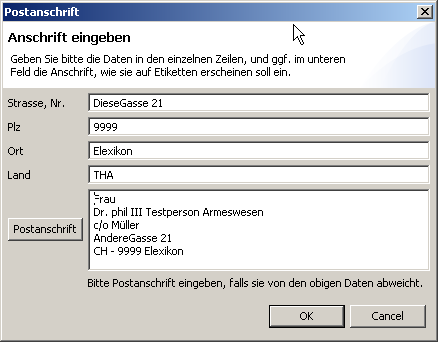
\includegraphics{images/anschrifteingabe}
  \caption{Anschrift-Eingabe}
  \label{fig:anschrift}
\end{center}
\end{figure}
\bigskip
\pagebreak[3]
\subsection{Artikel}
\label{view:artikel}
Ein \glqq Artikel\grqq{}ist jedes Objekt, das auf Lager genommen und/oder
abgegeben werden kann. Es gibt einerseits vordefinierte Artikel (z.B. die Liste
aller zugelassenen Medikamente), andererseits auch Eigenartikel. Elexis kann den
Lagerbestand von Lagerartikeln verwalten und halbautomatisch Bestellungen zur Neige
gehender Artikel vornehmen.


\subsection{Artikelliste}
In Abb. \ref{fig:artikel} ist eine Artikelauswahl-Liste und die
Artikeldetaildarstellung nebeneinander zu sehen.

 %\usepackage{graphics} is needed for \includegraphics
\begin{figure}[htp]
\begin{center}
  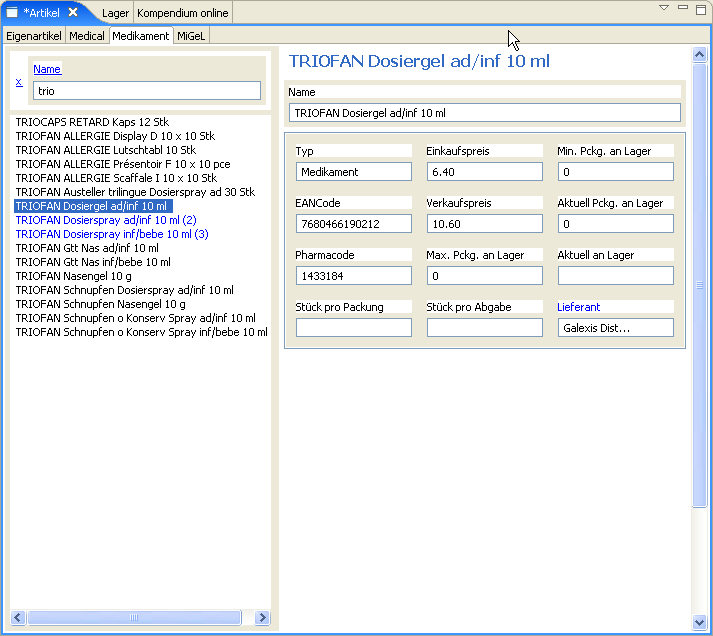
\includegraphics[width=0.9\textwidth]{images/artikelview}
  \caption{Artikel-View}
  \label{fig:artikel}
\end{center}
\end{figure}
Die Liste links können Sie in gewohnter Weise filtern, indem Sie einige
Buchstaben des gewünschten Artikelnamens eingeben.
In der Detailansicht sehen Sie Einzelheiten zum gerade ausgewählten Artikel. (In
Perspektiven, wo die Liste allein dargestellt ist, können Sie mit der rechten
Maustaste und \glqq Bearbeiten\grqq{} zur Detailansicht gelangen.)


Ein Artikel wird dadurch zum Lagerartikel, dass Sie ihm einen Mindestbestand
grösser als Null zuweisen. Geben Sie ausserdem einen Höchstbestand höher als der
Mindestbestand ein und weisen Sie dem Feld \glqq Istbestand\grqq{} den korrekten
Wert zu. Elexis wird bei einer halbautomatischen Bestellung von jedem Artikel,
dessen Istbestand unter dem Mindestbestand ist, soviele Exemplare bestellen, um
auf den Höchstbestand zu kommen.

Bei manchen Artikeltypen wird üblicherweise nicht eine ganze Verpackungseinheit
auf einmal abgegeben, beispielsweise Ampullen. Hierfür sind die Felder \glqq
Stück pro Packung\grqq{}und \glqq Stück pro Abgabe\grqq{}vorgesehen. Angenommen
ein Artikel wird in Packungen zu 10 Stück eingekauft, aber einzeln abgegeben.
In diesem Fall können Sie bei Stück pro Abgabe eine 1 setzen, bei Stück pro
Packung eine 10. Wenn dieser Artikel dann einem Patienten verrechnet wird, dann
wird automatisch 1/10 des Verpackungs-Verkaufspreises berechnet und auch nur
1/10 einer Packung aus dem Lager ausgebucht.

Die Angabe \glqq Aktuell an Lager\grqq{} meint dann die Zahl der einzelnen
Artikel, während \glqq Aktuell Pck. an Lager\grqq{} für die Zahl der
unangebrochenen Packungen steht.


\subsection{Lager und Bestellung}
Wie oben beschrieben, kann Elexis Ihr Warenlager halbautomatisch bewirtschaften.
Wann immer Sie einem Patienten einen Artikel verrechnen, wird dieser Artikel
automatisch aus dem Lagerbestand ausgebucht. Sobald der Bestand eines
Lagerartikels unter den von Ihnen definierten Mindestbestand fällt, \glqq
weiss\grqq{} Elexis, dass dieser Artikel nachbestellt werden muss. Nebst dieser
automatischen Erkennung können Sie selbstverständlich Bestellungen auch manuell
erstellen und/oder ändern.

Diese Funktionen sind in der View \glqq Bestellung\grqq{} erreichbar (s. fig.
\ref{fig:bestellungen}).
 %\usepackage{graphics} is needed for \includegraphics
\begin{figure}[htp]
\begin{center}
  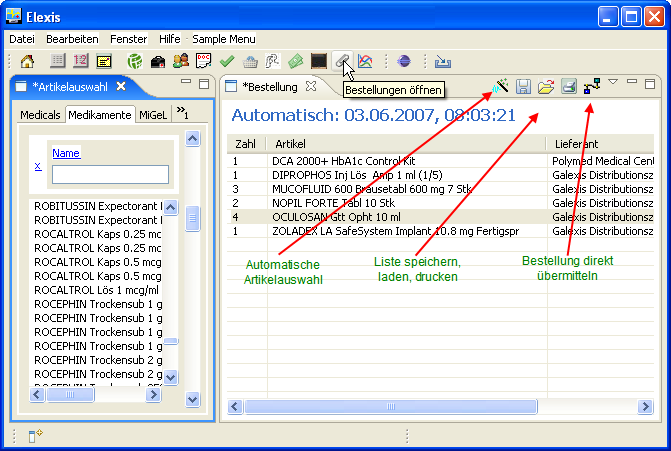
\includegraphics[width=0.9\textwidth]{images/bestell1}
  \caption{Bestellungen - View}
  \label{fig:bestellungen}
\end{center}
\end{figure}


Links finden Sie die schon bekannten Artikelauswahlfenster für alle
Artikelkategorien, für die Sie Plugins haben (Normalerweise Medikamente,
Medicals, MiGeL und Eigenartikel). Rechts ist das Feld Bestellung, welches
anfangs leer ist. Sie haben nun folgende Möglichkeiten:
\begin{itemize}
  \item Mit Klick auf das Zauberstab-Symbol werden automatisch diejenigen
  Artikel der Bestellung zugefügt, von welchen weniger als der Mindestbestand an
  Lager ist. Es werden jeweils soviele bestellt, dass der für diesen Artikel
  definierte Höchstbestand erreicht wird.
  \item Sie können aus einem der Fenster links Artikel in die Bestellung
  herüberziehen.
	\item Sie können auf einen der Artikel in der Bestelliste mit der rechten
	Maustase klicken, und den Artikel aus der Liste entfernen oder die Zahl ändern.
	
	\item Sie können die Bestellung erst mal abspeichern und später weiterbearbeiten.
	
	\item Sie können eine früüher gespeicherte Bestellung wieder laden.
	\item Sie können die Bestellung ausdrucken. Dafür ist eine System-Textvorlage (s. S.
	\pageref{textvorlagen}) namens \glqq Bestellung\grqq{} notwendig, welche an
	einer Stelle den Platzhalter [Bestellung] enthält (s. Abb. \ref{fig:bestell2}).
	\item Last but not least können Sie, falls Sie ein entsprechendes Plugin für
	Ihren Lieferanten haben, die Bestellung direkt via Internet oder Modem
	absenden. Ein entsprechendes Plugin für Galexis ist bereits verfügbar, weitere
	werden entwickelt.
\end{itemize}
\begin{figure}[hb]
  % Requires \usepackage{graphicx}
  
\includegraphics{images/bestell2}\\
  \caption{Ausschnitt aus der Vorlage Bestellung}\label{fig:bestell2}
\end{figure}

\subsection{codes}
Codes




	% *******************************************************************************
% * Copyright (c) 2007 by Elexis
% * All rights reserved. This document and the accompanying materials
% * are made available under the terms of the Eclipse Public License v1.0
% * which accompanies this distribution, and is available at
% * http://www.eclipse.org/legal/epl-v10.html
% *
% * Contributors:
% *    G. Weirich - initial implementation
% *
% *  $Id: konsviews.tex 4902 2009-01-03 10:47:34Z rgw_ch $
% *******************************************************************************
% !Mode:: "TeX:UTF-8" (encoding info for WinEdt)


\section{'Views' en rapport avec les consultations}



\subsection{Cas}
Cette view (Fig. \ref{fig:faelle2} létabli une liste de tout les cas du patient actuellement sélectionné. \index{Liste des cas}
\begin{wrapfigure}{l}{6.8cm}
  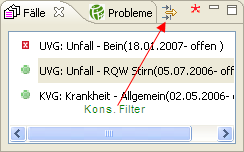
\includegraphics{images/faelleview}
  \caption{Fälle - View}
  \label{fig:faelle2}
\end{wrapfigure}

Le symbole qui se trouve à gauche de la désignation du cas indique si toutes les données nécessaires ont été rassemblées pour que la facturation puisse être faite : S'il est vert, l'établissement de facture devrait être possible, s'il est rouge, manque encore une ou plusieurs données.


\textit{Quelles} indications minimales sont nécessaires, dépend du système de facturation. Ainsi, pour les cas qui sont facturés selon la LAMal,l'indication d'un destinataire de la facture, d'un 	assureur et du numéro d'assurance est nécessaire. Les cas qui sont comptabilisés selon la LAA nécessitent un numéro de cas. Pour des factures en privé un destinataire de la facture devra au moins être indiqué.

\medskip

\index{filtrer!consultations}
\label{filter:fall}
Un clic sur le symbole de filtre dans l'entête de la 'View' a pour conséquence qu'il n'y a plus que les consultations dans la liste de consultation (cf \ref{view:konsultationen}) qui font partie du cas choisi actuellement. Si on choisi un autre cas, la liste est de nouveau filtrée. Cliquez encore une fois sur le symbole de filtre pour éteindre le filtre.

Le clic droit sur un cas ouvre son menu de contexte. Celui-ci contient les points
suivants :

\begin{itemize}
  \item {Supprimer un cas}. Ceci n'est possible, que si vous avez les droits nécessaires, et si plus aucune consultation n'existe .
  \item {Modifier un cas }. Ceci ouvre une autre 'View', dans laquelle les détails pour le cas actuellement séléctionné peuvent être introduits.
  \item {Réouverture du cas}. Ceci permet de réactiver un cas déjà fermé. \footnote{Un cas est fermé si une date de fin a été introduite. On ne peut plus ajouter une consultation à un cas fermé.}
  \item {Créer une facture}. Par ceci, une facture peut être produite qui concerne toutes les consultations non comptabilisées du cas actuel et du mandant actuel. Il s'agit d'un \glqq raccourci\grqq{} du procédé normale de l'établissement de facture qui convient surtout pour l'établissement immédiat de différentes consultations ou prestations.
\end{itemize}


\clubpenalty=5000

\subsection{Cas et consultations}
 %\usepackage{graphics} is needed for \includegraphics
\begin{wrapfigure}{l}{7cm}
  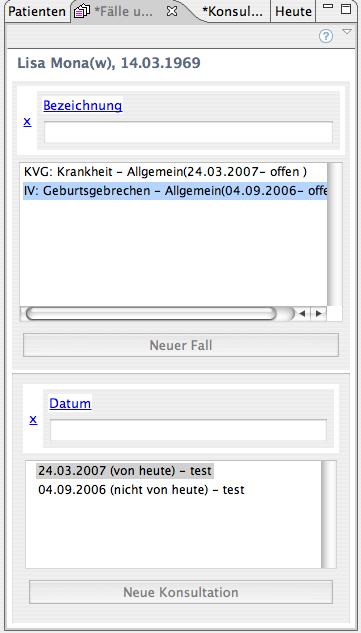
\includegraphics[width=7cm]{images/fallkonsview}
  \caption{Fälle und Kons}
  \label{fig:fallkons}
\end{wrapfigure}
Cette View (Fig. \ref{fig:fallkons} montre une liste synoptique des cas et des consultations correspondantes (seulement titres sans textes). Si on choisi dans le secteur supérieur un cas en cliquant dessus, les consultations correspondantes de ce cas sont indiquées dans le secteur inférieur.
Si on clique sur une consultation elle sera affichée dans la 'View' - consultation.
(cf page \ref{konsview} s. \pageref{konsview})

Pour établir un nouveau cas introduisez un titre pour ce cas et cliquez sur \textit{nouveau cas}. Pour une nouvelle consultation choisissez le cas concerné et cliquez sur  \textit{nouvelle consultation}

\medskip

Remarque : Vous avez constaté que cette 'View' et la View 'Cas' traité antérieurement sont jusqu'à un certain point redondantes. C'est ainsi. Vous pouvez préférer des 'Views' séparés pour les 'Cas' et les 'Consultations' ou favoriser une seule 'View' qui contient les deux. En général, vous n'appliquerez pas les deux concepts en même temps, mais celui qui vous convient mieux - Elexis vous laisse le choix.


\clearpage

\subsection{Historique des Consultations}
\label{view:konsultationen}
\begin{wrapfigure}{L}{7.5cm}
  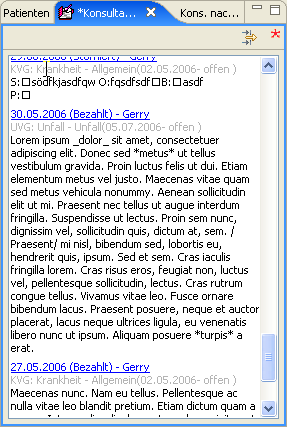
\includegraphics{images/konslisteview}
  \caption{Konsultationsliste}
  \label{fig:konslisteview}
\end{wrapfigure}

Ceci est une énumération de toutes les consultations précédentes du patient actuellement sélectionné, indépendamment du cas respectif.
\index{liste des consultations} Pour chaque consultation le texte est affiché sans formatages. (cf Fig.\ref{fig:konslisteview}).\\
En cliquant sur le titre (bleu) d'une consultation vous choisissez cette consultation dans la 'View Consultation' (cf page \pageref{konsview}).

En cliquant sur le symbole du filtre à droite en haut vous ouvrez la fenêtre du dialogue du filtre (cf Fig. \ref{fig:konsfilter}).
\index{Filtre consultations} C'est ici que vous pouvez introduire les critères selon lesquels les consultations devraient être filtrées avant d'être affichées (que les consultations qui correspondent aux conditions du filtre soient affichées).
Dans le champ supérieur vous pouvez indiquer si seulement des consultations d'un certain cas ou si tous les cas doivent être affichés. Dans le champ  inférieur, vous pouvez suggérer les critères de recherche qui doivent exister dans le texte de la consultation. Plusieurs termes de recherche peuvent ainsi être liés avec AND, OR, NOT,AND NOT et OR NOT.

Par exemple si on introduit \glqq Lorem AND NOT ipsum\grqq{} on ne trouve que les consultations dont le texte contient  \glqq Lorem\grqq, mais pas \glqq ipsum\grqq{}.

Tout en bas vous pouvez enfin encore indiquer si l'écriture majuscule/minuscule doit être considérée, ou si des critères de recherche doivent être considérés comme des termes fixes. Une explication précise de ce thème irait ici trop loin ; à ce sujet vous pouvez trouver beaucoup de littérature en utilisant les mots de recherche \glqq Regular
Expression\grqq{}ou \glqq Pattern Matching\grqq{}. Cette technique permet de décrire le critère de recherche avec différents caractères de remplacement. Ainsi permet p. ex.\glqq M[ae][iy]e?r\grqq{} de chercher tous les Meiers, Mayrs etc. donc toutes les formes d'écritures.

\medskip

Remarque : 
Filtrer l'historique par cette procédure peut durer quelques secondes, puisque le texte de chaque consultation doit être fouillé complètement. Si on veut filtrer seulement d'après des cas ou des problèmes, le filtre par cas correspondant  (cf \pageref{filter:fall}) ou le filtre de liste de problème  (cf \pageref{filter:problemliste})est en général plus efficace.

\begin{figure}[ht]
\begin{center}
  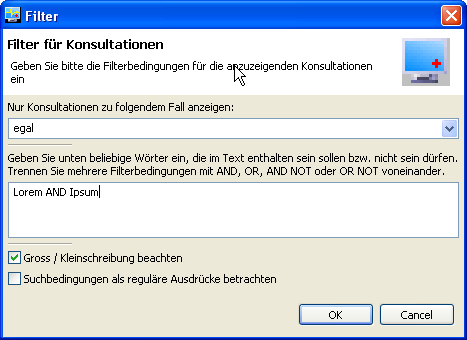
\includegraphics{images/filterdialog}
  \caption{Filterdialog}
  \label{fig:konsfilter}
\end{center}
\end{figure}


\subsection{Consultation}
 \label{konsview}
Aperçu détaillé d'une saisie de consultation(cf Fig. \ref{fig:konsdetail}).
\begin{figure}[ht]
  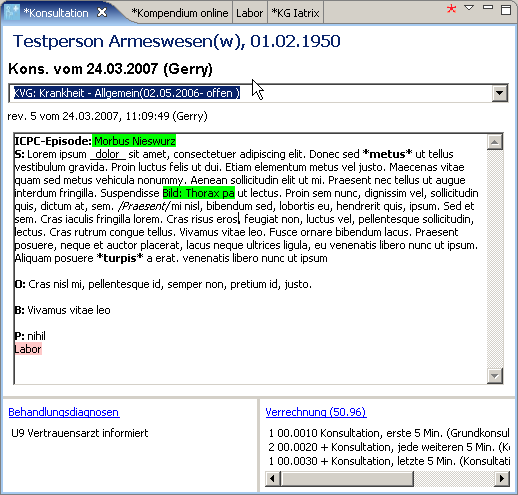
\includegraphics{images/konsview}
  \caption{Konsultation: Detail}
  \label{fig:konsdetail}
\end{figure}

Vous trouvez dans la zone de texte les possibilités supplémentaires suivantes :
\begin{description}
\item[Makros]
Ecrivez un texte quelconque, marquez-le avec la touche gauche de la souris, cliquez ensuite avec la touche droite de la souris et choisissez  'comme macro…' . Donnez un nom arbitraire à la macro. Si vous tapez à l'avenir le nom de la macro suivi d'un \# le texte prédéfini de la macro est introduit dans le texte.

\item[Introduire des prestations]
Si vous tapez le nom d'un bloc de prestation suivi d'un \#, ce bloc est comptabilisé comme si vous l'aviez tiré avec la souris dans au champ de facturation.


\item[Commandes du texte ]
Il est possible d'introduire quelques commandes simples du texte:
Un mot au début d'une ligne qui est suivi d'un deux-points se présente en caractères gras, la même chose est le cas pour mot entre deux  *. Un mot entre deux  / est écrit en italique.
\end{description}


\subsection{Certificat d'incapacité de travail}
Cette 'View' sert à fixer une incapacité de travail . (Fig. \ref{fig:auf})
\index{Certificat} \index{Certificat d'incapacité de travail}.
\begin{figure}
  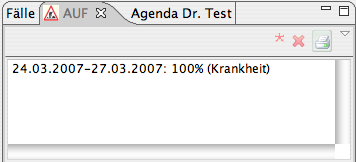
\includegraphics{images/aufview}
  \caption{AUF-View}
  \label{fig:auf}
\end{figure}
Une incapacité de travail se réfère toujours à un cas spécifique. Si aucun cas est marqué, vous serez d'abord invité d'en marquer un.

Si vous cliquez sur le symbole  \glqq nouveau\grqq (bouton vert avec un plus blanc), il apparaît une fenêtre dans laquelle vous pouvez fixer le début et la fin de l'arrêt de travail de même que le pourcentage de l'incapacité.
En cliquant sur le symbole de \glqq l'imprimante \grqq, une 'View'-Texte s'ouvre où vous pouvez effectuer encore manuellement des adaptations du texte du certificat avant de l'imprimer ou de le faxer.

\subsection{Ordonnances}
Dans cette 'View' les ordonnances seront enregistrées.  \index{ordonnance} Cliquez sur le symbole\glqq nouveau\grqq
(bouton vert avec un plus vert) pour créer une nouvelle ordonnance avec la date actuelle. Tirez les articles (médicaments) par 'Drag and Drop' d'une liste d'article ou de la 'View de médication à long terme' dans cette ordonnance. En cliquant sur le symbole \glqq imprimante\grqq vous ouvrez une 'texte-View' dans laquelle vous pouvez encore faire des modifications manuelles avant d'envoyer l'ordonnance définitivement vers l'imprimante ou un appareil de télécopie ou vers un connecteur d'exportation. Pour tout cela un modèle avec le nom  \glqq Ordonnance\grqq
doit avoir été crée qui contient un espace réservé [lignes de prescription] dans lequel les articles choisis sont insérés.


\subsection{Détails du cas}
\label{falldetail}
\index{Détails du cas}
 Cette 'View' (Fig. \ref{fig:falldetail}) sert à ajuster les détails d'un cas (une boîte de dialogue avec la même View est ouverte, s'il faut ouvrir un nouveau cas( cf \ref{definition:fall} page \pageref{definition:fall})).
\begin{figure}[ht]
  % Requires \usepackage{graphicx}
  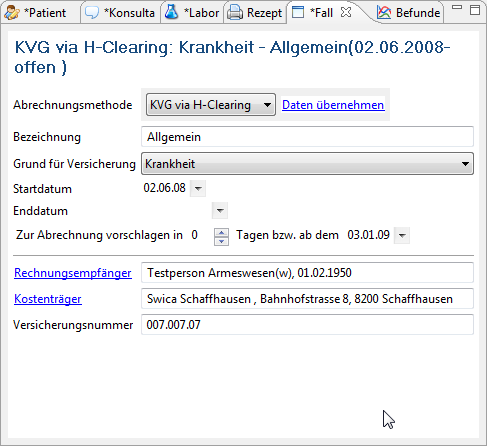
\includegraphics[width=0.8\textwidth]{images/falldetail}\\
  \caption{Fall-Detail}\label{fig:falldetail}
\end{figure}
Indiquez dans la boîte de choix en haut quel système de facturation doit être appliqué pour ce cas (cf aussi \ref{settings:abrechnungssystem} page \pageref{settings:abrechnungssystem}). En dessous il y a un espace où vous pouvez choisir librement une désignation pour le cas. Celui-ci ne sert qu'à vos propres informations, afin que
 vous puissiez mieux distinguer les différents cas du même patient.
La prochaine ligne, 'la raison pour l'assurance' est une indication qui apparaîtra sur les factures qui concernent le cas (si jamais le modèle de facturation contient un champ spécifique pour cela).

La\textbf{date de départ } est généralement la date de la première consultation, ou en cas d'accident, la date de l'accident. La  \textbf{date finale } désigne la date quand le cas est terminé. Un cas qui a une date de fin, est marqué comme 'cas terminé' dans la liste des cas  (Fig. \ref{fig:faelle2}) . Le cas terminé ne permet plus de ajouter une consultation de plus. 
Généralement, un cas ne devrait être terminé que s'il s'agit d'un accident qui est terminé, ou si le patient change d'assureur et si les données de facturation changent pour cette raison.

La prochaine ligne, destinataires de la facture, est impérative, afin qu'une facture puisse effectivement être fournie. Cela doit être un contact déjà existant (p. ex. le patient lui-même).

\medskip
Toutes les autres lignes seront selon le choix du système de facturation différentes. Souvent il y existera aussi une ligne 'répondant des coûts' \footnote{Remarque importante : Pour le \textbf{système Tarmed } (Suisse): Si le destinataire de la facture et le répondant des coûts est identique, une facture Tiers-Payant est fourni, autrement une facture Tiers-garant . Veillez ainsi à ce que ces deux lignes soient correctes (Pour des cas LAA les assureurs d'accident doivent être les destinataires de la facture et en même temps répondants des coûts tandis qu'avec les cas LAMAL le patient est destinataires de la facture dans les cantons Tiers garants et la caisse de maladie est répondant des coûts.)}.

\clearpage

\subsection{Diagnostics}
\label{view:diagnosen} \index{Diagnostics}
Cette 'View' (Fig. \ref{fig:diagnosen}) sert à choisir des diagnostics et de les assigner aux consultations respectives. \begin{wrapfigure}{l}{7cm}
    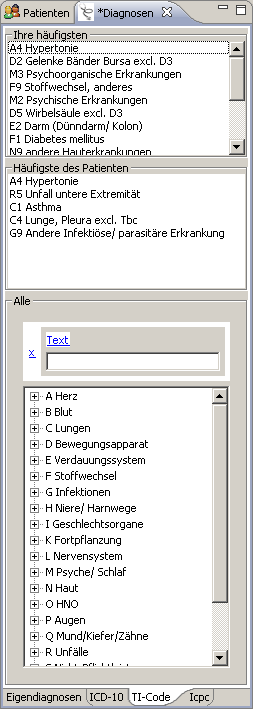
\includegraphics[width=6.5cm]{images/diagnosenview}
    \label{fig:diagnosen}
    \caption{Diagnosen-Auswahl}
\end{wrapfigure}
Vous voyez vers le bas une série d'onglets qui correspondent aux Plugins de code de diagnostic installés. (comme standard : Code tessinois, CIM-10, et CISP-2). Pour choisir un diagnostic vous choisissez d'abord entre ces onglets le système de codification correspondant et ensuite le code.
Le choix peut avoir lieu par 'Drag and Drop' ou par double-clic .
Vous voyez pour chaque système de codification, une fenêtre divisée en trois : Dans le secteur supérieur se trouvent vos diagnostics les plus fréquemment utilisés (c.-à-d. de l'utilisateur actuellement connecté) ; dans la partie moyenne se trouvent les diagnostics qui ont jusqu'ici le plus fréquemment été utilisés pour le patient en question et dans la partie inférieure se trouve la systématique entière du système de codification choisi.



\medskip

De cette façon vous avez toujours accès aux codes des diagnostics les plus fréquemment utilisés et vous n'auriez que rarement à fouiller la systématique entière.


	% *******************************************************************************
% * Copyright (c) 2007 by Elexis
% * All rights reserved. This document and the accompanying materials
% * are made available under the terms of the Eclipse Public License v1.0
% * which accompanies this distribution, and is available at
% * http://www.eclipse.org/legal/epl-v10.html
% *
% * Contributors:
% *    G. Weirich - initial implementation
% *
% *  $Id: laborview.tex 2932 2007-07-29 06:21:06Z rgw_ch $
% *******************************************************************************
% !Mode:: "TeX:UTF-8" (encoding info for WinEdt)

\section{Laboranzeige-View}
\index{Labor!Eingabe}
\index{Labor!Anzeige}
Bei Elexis werden sowohl interne als auch externe Laborbefunde, sowohl
automatisch eingelesene als auch manuell eigegebene Befunde in derselben Sicht
angezeigt.

Die  Anzeige eines Befundes wird bestimmt durch
\begin{itemize}
  \item Ein Laboritem, zu dem dieser Befund gehört
  \item Ein Datum, an dem dieser Befund erhoben wurde
  \item Einen Patienten, zu dem dieser Befund gehört
\end{itemize}

Das Laboritem definiert, wie und wo der Laborbefund angezeigt werden soll, und
zu welchem Typ von Laborwerten er gehört. Das Erstellen von Labritems ist in der Regel nur bei der Installation des
Programms notwendig, bzw. dann, wenn Sie neue Laborparameter in Ihre
Standardbesimmungen aufnehmen möchten. Das genaue Vorgehen ist unter Konfiguration (S. \pageref{config:labor} genauer beschrieben.

 %\usepackage{graphics} is needed for \includegraphics
\begin{figure}[htp]
\begin{center}
  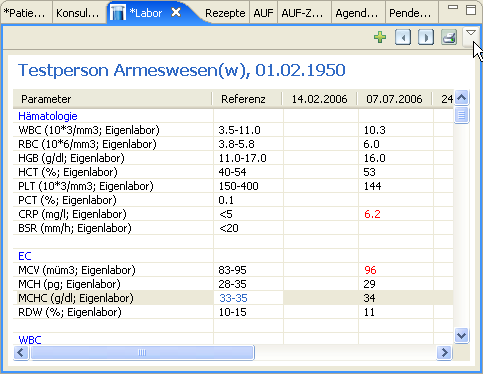
\includegraphics{images/labview}
  \caption{Labor-Anzeige}
  \label{fig:labview}
\end{center}
\end{figure}

\subsection{Manuelle Eingabe}
Um Laborwerte manuell einzutragen, gehen Sie so vor:
\begin{itemize}
    \item Wenn für das gewünschte Datum noch keine Spalte exstiert, klicken Sie auf das grüne Pluszeichen rechts oben, um ein Datum anzugeben.
    \item klicken Sie auf die Zeile und Spalte, wo Sie einen Laborwert eingeben möchten. Tippen Sie den Wert ein und verlassen Sie das Feld mit der Eingabetaste, oder der Pfeil-nach-unten-Taste.
\end{itemize}
Wenn ein Laborparameter numerisch ist, und der eingegebene Wert ausserhalb des Referenzbereichs ist, wird der Wert in rot angezeigt. Sie können diese Anzeige auch manuell ein- und ausschalten, indem Sie den Wert mit der rechten Maustaste anklicken und das Häkchen vor \glqq pathologisch\grqq{} setzen oder löschen.

\subsection{Automatisches Einlesen}
\index{Labor!automatisches Einlesen}
Elexis kann Laborwerte selbstverständlich auch automatisch einlesen. Hierfür dient das View-Menu rechts oben:\\
\begin{wrapfigure}{r}{7cm}
    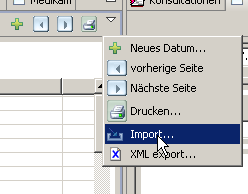
\includegraphics{images/labor6}
\end{wrapfigure}
Klicken Sie auf \textit{import} und wählen Sie in der dann erscheinenden Dialogbox die Quelle für die einzulesenden Laborwerte aus. Was für Quellen hier angeboten werden, hängt von den vorhandenen Laborimport-Plugins ab. In Frage kommen Laborgeräte und verschiedene externe Labors. Eine aktuelle Liste aller vorhandenen Laborimport-Plugins finden Sie auf http://www.elexis.ch

\subsection{Laborblatt drucken}
Um ein Laborblatt auszudrucken, klicken Sie auf das Drucker-Symbol rechts oben. Dies erstellt eine Tabelle innerhalb einer System-Textvorlage \glqq Laborblatt\grqq{}, welche einen Platzhalter [Laborwerte] enthalten muss (s. auch \ref{textvorlagen}).

\section{Labor Neu}
Diese View dient dazu, alle Laborwerte anzuzeigen, welche noch nicht als \glqq gesehen\grqq{} markiert worden sind, und erlaubt es auch gleich, sie als gesehen zu markieren (S. Abb. \ref{fig:labneu}).

\begin{figure}
  % Requires \usepackage{graphicx}
  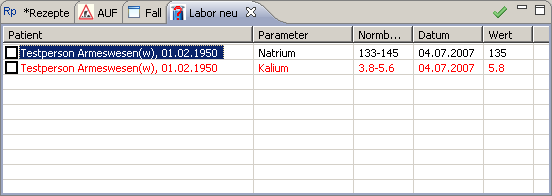
\includegraphics{images/labneu1}\\
  \caption{Anzeige neuer Laborwerte}\label{fig:labneu}
\end{figure}

Werte ausserhalb des Referenzbereichs werden rot dargestellt. Man kann gesehene Werte mit einem Häkchen in der Checkbox links markieren. Nach einiger Zeit werden diese dann aus der Liste entfernt (Solange sie noch nicht entfernt sind, kann man die Markierung mit einem erneuten Klick wieder löschen).

Mit einem Klick auf das grüne Häkchen-Symbol rechts oben kann man alle angezeigten Werte gleichzeitig als gesehen markieren.

Um die Werte einzeln oder gesamthaft als gesehen zu markieren, ist das Recht \textit{Daten/Patient/Labor abhaken} erforderlich (s. \ref{sec:gruppen}, S. \pageref{sec:gruppen}ff.)

	% *******************************************************************************
% * Copyright (c) 2007 by Elexis
% * All rights reserved. This document and the accompanying materials
% * are made available under the terms of the Eclipse Public License v1.0
% * which accompanies this distribution, and is available at
% * http://www.eclipse.org/legal/epl-v10.html
% *
% *  $Id: abrechnung.tex 4911 2009-01-05 17:56:39Z rgw_ch $
%
%*******************************************************************************
% !Mode:: "TeX:UTF-8" (encoding info for WinEdt)

\section{'Views' en relation avec la facturation}
\subsection{Consultations selon date}
\begin{wrapfigure}{l}{7.3cm}
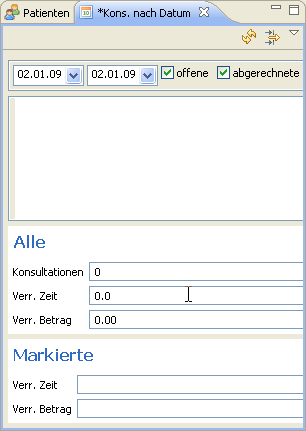
\includegraphics[width=7cm]{images/heute}
\caption{Konsultation nach Datum}
\label{fig:heute}
\end{wrapfigure}

Cette View (Fig. \ref{fig:heute}) sert à afficher les consultations d'une certaine période (normalement celles du jour actuel). Elle donne un aperçu de facturation et du temps calculé pour chaque consultation en particulier et aussi du total. En cliquant sur la 'check-box', vous pouvez laisser calculer des consultations ouvertes \footnote{il s'agit de celles qui n'ont pas encore été facturées} ou clôturées ou les deux. Vous pouvez indiquer dans les champs de date le début et la fin de la période en question. Après chaque modification vous devez utiliser le bouton 'actualiser liste' pour que la liste sera calculée à nouveau.

\medskip

Dans la section inférieure de la 'View' vous apercevez le nombre total des consultations au cours de la période choisie, ainsi que (défini par le système de codage de prestation) le temps et le montant comptabilisé. Dans le champ dessous vous voyez les mêmes indications pour la consultation actuellement marquée en bleu.

Vous pouvez donc utiliser cette 'View' aussi pour pouvoir passer revu le soir
toutes les consultations de la journée et pour introduire les prestations ou pour les corriger.


\medskip

En outre, cette 'View' permet des fonctions statistiques simples :
%\begin{itemize}
Si vous cliquez sur le bouton 'filtre', une boîte de filtre s'ouvre dans la partie supérieure de la 'View'. Depuis une fenêtre de facturation vous pouvez tirer les positions que vous voulez prendre en compte vers cette boite. Lors de la prochaine actualisation de la liste, la 'View' ne calculera que des consultations dans lesquelles apparaît au moins un des codes de positions souhaités. Les codes et les sommes totales seront alors énumérés séparément (lors de l'impression, voir ci-dessous).

\medskip

Dans 'view-menu' vous trouvez l'option 'imprimer liste'. En cliquant dessus, une fenêtre s'ouvre contenant un tableau qui énumère et fait imprimer les consultations indiquées.

\medskip

Pour des statistiques plus détaillées vous pouvez choisir aussi dans la'view-menu' l'option 'statistiques'. Ceci fourni un fichier en format CSV\footnote{Character Separated Values : un format standard pour des fichiers sous forme de tableau} qui peut être lu et statistiquement conditionné par des programmes comme OpenOfficde.org calc ou Microsoft\texttrademark Excel\texttrademark Ce fichier contient toutes les positions comptabilisées avec fréquence, coûts et chiffre d'affaire.


\subsection{Consultations à facturer}
\index{facturation} Cette View (cf Fig. \ref{fig:konsv})sert à choisir les consultations, dont une facture doit être établie.
Ceci concerne seulement les consultations du mandant actuel.

\begin{figure}[hb]
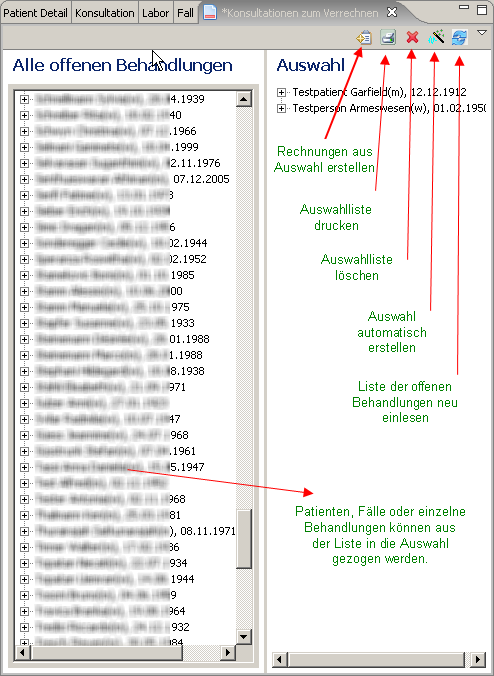
\includegraphics{images/konsv}
\caption{Konsultation zur Verrechnung auswählen}
\label {fig:konsv}
\end{figure}
Pour cela il y a des possibilités suivantes :
\begin{itemize}
  \item Choix automatique (Icône de baguette magique) : Les consultations à facturer sont choisies automatiquement d'après certaines règles et transférées dans la liste de choix. Cela sera expliqué ci-dessous plus précisément (facturation automatique).
  \item Tirer le nom du patient vers la liste de choix : Toutes les consultations concernant tous les cas (LAMAL , LAA etc) du patient choisi sont marquées pour être facturées.
  \item Tirer des cas (LAMA ; LAA etc) depuis la liste vers la liste de choix : Toutes les consultations des cas choisis sont marquées pour être facturées.
  \item Tirer des consultations depuis la liste vers la liste de choix : Seulement les consultations choisies sont marquées pour être facturées.
\end{itemize}
Avec toutes les méthodes mentionnées vous pouvez librement modifier votre choix postérieurement. Vous pouvez ajouter d'autres éléments, ou vous pouvez éliminer des éléments (après clic droit sur un élément dans la liste de choix), ou vous pouvez supprimer même le choix entier. A ce moment là il n'y a pas encore eu de modification des données .

Si vous avez fini de choisir vous pouvez cliquer sur  \glqq établir les factures\grqq pour que les factures pour tous les éléments présents dans le choix soient établies. Toutes les consultations qui font partie d'un cas sont toujours résumées. Plusieurs factures sont ainsi fournies si plusieurs cas d'un patient  se trouvent dans la liste de choix.

\subsubsection{Facturation automatique}
\index{Facturation automatique}\label{auto}
Par cette méthode la facturation des consultations suit des critères spécifiquement déterminés auparavant  (cf Fig. \ref{fig:rnautomatik}).
\begin{figure}
  % Requires \usepackage{graphicx}
  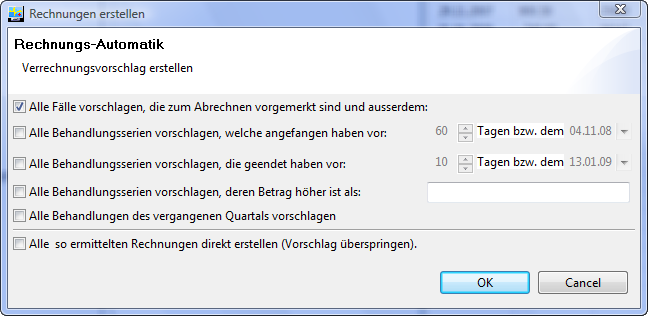
\includegraphics[width=1.0\textwidth]{images/rechnungsautomatik}\\
  \caption{Halbautomatischer Rechnungsvorschlag}\label{fig:rnautomatik}
\end{figure}

\begin{itemize}
\item Proposer tout les cas qui sont retenu pour la facturation : Si vous cliquez cette 'check-box' les consultations des cas seront choisis pour lesquels vous avez spécifié une date de facturation dans les détails du cas. (voir Fig. \ref{fig:falldetail}).
\item Proposer toutes les séries de traitement qui ont commencé avant le … : Choisit toutes les consultations non facturées d'un cas (LAMA, LAA etc) jusqu'aujourd'hui à condition qu'au moins une consultation avait eu lieu avant la date limite.
\item Proposer toutes les séries de traitement qui ont été terminées avant le … : Choisit toutes les consultations non facturées d'un cas (LAMA, LAA etc) à condition que la dernière consultation avait eu lieu avant la date limite.
\item Proposer toutes les séries de traitement dont la somme est plus grande que … : Choisit toutes les consultations non facturées d'un cas (LAMAL, LAA etc) à condition que la somme totale de la facture dépasse le montant choisi.
\item Proposer la facturation de tous les traitements du trimestre passé : Facturation du dernier \textit{trimestre} selon le calendrier avec les dates limites suivantes : 31.3 ; 30.6 ; 30.9 et 31.12.
\end{itemize}
S'applique à toutes les options : N'est exploitée seulement lorsque le crochet est mis dans la 'check-box'. Il ne suffit donc pas de seulement introduire une valeur. Les différentes options s'appliquent de façon additive : Finalement toute consultation est choisie pour la facturation à la quelle s'applique au moins un des critères actifs.

\medskip

\clearpage

\subsection{Factures}
\begin{figure}[ht]
  % Requires \usepackage{graphicx}
  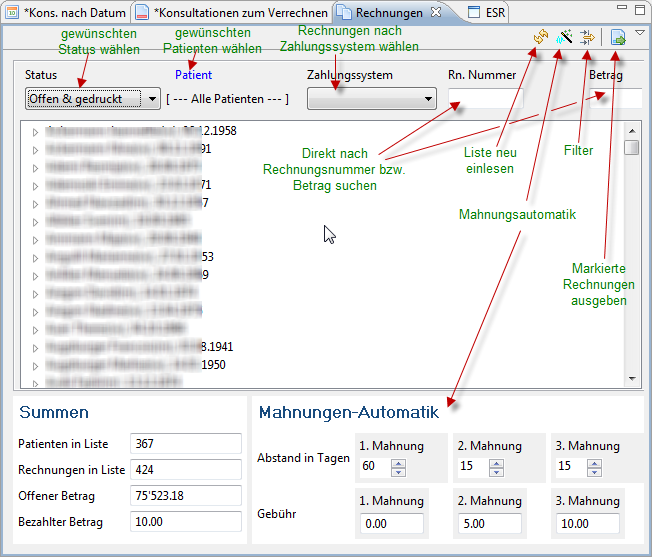
\includegraphics[width=1.0\textwidth]{images/rechnungsview}\\
  \caption{Rechnungen-View}\label{fig:rechnungen}
\end{figure}

Dans cette 'View' (Fig. \ref{fig:rechnungen})vous voyez les factures établies. Une facture a toujours un 'état' spécifique :
\begin{description}
    \item [Ouvert] immédiatement après la facturation. 
    \item [Ouvert et imprimé ] La facture avait été édité au moins une fois (soit par impression soit par une autre méthode d'exportation). A partir de ce moment le délai de payement commence à s'écouler. (Toutefois Elexis ne peut pas constater si par exemple une facture n'a pas été correctement imprimé ou si elle n'avait pas été envoyée. Pour cette raison se trouve ici une source d'erreurs potentielle.)
    \item[Rappel] Le rappel a été établi mais pas encore imprimé.
    \item[Rappel imprimé ] Le rappel a été imprimé.
    \item [2ième Rappel établi, 2ième Rappel imprimé, 3ième Rappel établi, 3ième Rappel imprimé ]: en analogie
    \item[Payement partiel ] Il y a au moins un payement mais qui ne couvre pas la totalité de la facture.
    \item[payée] La facture a été entièrement payée par un ou plusieurs paiements.
    \item [payé trop] ça peut aussi arriver pour une fois ;-)
    \item [Perte partielle ] Une partie de la facturation est définitivement mise dans les pertes (Contrairement à la situation du  \glqq payement partiel \grqq{} vous ne comptez plus avec un payement de plus)
    \item [Perte totale] La facture entière fait partie des pertes. 
    \item [En poursuite ] exactement ça
    \item [Annulé ] Une fois une facture établie, elle ne peut plus être supprimée. Cela doit être ainsi car sinon il serait possible que quelqu'un réclame une facture qui n'existe plus ou que quelqu'un veut des renseignements concernant une facture inexistante. Lorsqu'une facture est invalide pour une raison quelconque (erreurs, exonération du montant etc.) elle doit être annulée. L'annulation d'une facture a dans tous les aspects pratiques le même effet qu'une suppression à part du fait que le numéro de facture reste attribué et que la facture peut être examinée plus tard encore.
    \item [faux] Si un module de facturation constate qu'une facture contient des fautes (par ex. le module Trust-X pourrait réclamer qu'il y manquent certaines numéros EAN) la facture concernée reçoit le signe 'faux' et peut donc être corrigée.
    \item [à imprimer] Toutes les factures encore ouvertes mais pas encore imprimées de même que les rappels pas encore imprimés se trouvent dans cet état.
    \item [encours des crédits ] L'ensemble de tout des factures 'ouvertes et imprimées' , des 'rappels imprimés', des '2ième rappel imprimé' des '3ième rappel imprimé' des 'payements partiels' et des factures 'en poursuite'. Il s'agit donc de toutes les factures dont vous attendez encore un payement.
    \item [Stop des rappels ] exactement ça
\end{description}

La liste de facturation peut être sélectionné selon des différents critères. Pour mettre à jour la liste avec les données modifiées veuillez cliquer sur le bouton 'actualiser liste'. Pour afficher les factures d'un certain état veuillez choisir l'état en question sur le menu déroulant en haut à gauche sous 'état' (cf Fig. \ref{fig:rechnungen}). Pour afficher que la facture d'un patient spécifique cliquez sur \glqq patient\grqq{}. La boite de dialogue s'affiche pour vous laisser choisir les contacts. Introduisez la nom du patient et sélectionnez-le ensuite sur la liste. Cliquez sur o.k ou sur annuler pour retourner à l'affichage de la liste de tout les patients.

Pour ne choisir qu'un numéro de facture spécifique veuillez entrer le numéro dans le champ 'No de facture' et appuyez sur la touche 'Entrée' ou cliquez sur 'actualiser liste'.  Pour chercher une facture avec un montant spécifique (par ex. pour classer un payement de provenance non connue veuillez introduire le montant et poussez la touche d'entrée.

\medskip
Si vous cliquez sur le symbole 'filtre' vous recevez des options supplémentaires concernant l'affichage. 

\begin{wrapfigure}{l}{7cm}
\includegraphics[width=7cm]{images/rechnungsfilter}
\end{wrapfigure}
Les champs 'Montant : de  - à' servent à filtrer une somme spécifique. Vous pouvez aussi remplir qu'un des deux champs de sorte que l'autre devienne un limitation ouverte.
 Les champs \glqq date de facturation de\grqq{} et \glqq date de facturation jusque\grqq{} servent à chercher des factures uniquement émises entre les deux dates mentionnées. Par contre les champs  \glqq dates d'état : de - à\grqq{} permettent à filtrer des factures dont la dernière modification d'état se trouve entre les deux dates introduites. Aussi ici vous pouvez remplir un seul champ et laisser l'autre ouvert. 
 Si vous sortez de ce dialogue en cliquant sur OK, la liste sera actualisés selon vos nouveaux critères.

\medskip

Tant que le bouton 'filtre' reste enclenché toutes les 'actualisations de liste' seront liés avec le Filtre ET. Si vous filtrez par exemple la date 'd'état' jusqu'au 30.10.2007 et vous cliquez après dans le menu déroulant sous 'état' sur '2ième rappel imprimé' et vous appuyez sur le bouton 'actualiser liste', vous trouverez toutes les factures qui avaient été mises avant le 30.10.2007 dans l'état '2ième rappel imprimé'. 

En bas de cette fenêtre vous voyez la quantité de factures qui remplissent ces conditions et les sommes les concernant.

\subsubsection{'View-menu' de la liste des factures}
Le 'View-menu' (triangle à droite en haut, cf Fig. \ref{fig:rechnungen}) a des options suivantes :
\begin{description}
\item [Affichage complet / Affichage réduit ] Montre toutes les donnés en détail ou les réduit aux titres.
\item [Imprimer liste ] Imprime une liste de tout les patients respectivement factures qui sont marquées dans l'affichage actuel. Pour cette action il faut qu'il y existe un modèle d'impression pour le système nommé 'liste' qui contient un champ (liste).
\end{description}
\subsubsection{Changer une facture}
Vous pouvez changer la facture si vous cliquez avec la touche droite de la souris sur une facture dans la liste :
\begin{description}
\item [Facturer] Facturer une facture séparée. (v. ci-dessous)
\item [Comptabiliser paiement ] Vous pouvez introduire ici les paiements manuellement . Par exemple des paiements comptants ou les paiements par acompte. (Normalement la comptabilisation par fichier ESR se fait automatiquement).
\item [Ajouter émolument ] Ajouter manuellement par ex. les frais de rappel.
\item [Changer l'état ] On peut changer l'état de la facture manuellement. Elexis reconnaît la majorité des changements de l'état d'une facture. Ainsi change l'état des factures payées automatiquement sur  \glqq payée\grqq{} lorsqu'un fichier ESR de la banque est comptabilisé. Certains changements de l'état ne peuvent se faire que manuellement. Par exemple : Elexis ne peut par distinguer automatiquement entre \glqq paiement partiel\grqq{} et \glqq perte partielle\grqq{} puisque ceci doit être lié à une décision du créancier. La même chose vaut pour les factures \glqq En poursuite\grqq{} et la \glqq perte totale\grqq{}.
    A part de ça il faudra toujours être prudent avec des changements manuelles de l'état d'une facture car il n'y se font pas de corrections de comptabilisation.
\item [Augmenter le niveau de rappel] Ceci augmente le niveau de rappel d'une étape jusqu'au maximum du 3ième rappel.
\item [Annuler] Ceci permet d'annuler une facture. Il y existe la possibilité de débloquer certains traitements (lorsque la facture était erronée et doit être refaite) ou de les laisser bloqués (si le traitement ne doit définitivement pas être facturé).
\end{description}

\subsubsection{Facturation}
Par le bouton  \glqq facturation\grqq{} toutes les factures sélectionnées seront facturées. (Pour sélectionner une facture cliquez avec la touche gauche de la souris sur la facture. Pour sélectionner plusieurs factures sur la liste cliquez sur ces factures en tenant enfoncée en même temps la touche CTRL (ou MAC). Pour marquer toute une rangée de factures cliquez d'abord sur la première facture et après, en tenant la touche SHIFT, sur la dernière facture de la rangée.) Elexis ne facturera donc \textit{pas} toute la liste mais seulement les factures sélectionnées de la liste !


Les cibles possibles de la facturation dépend des différents 'Plugins de facturation' installés.
La cible peut par exemple être une imprimante qui imprime des factures selon TARMED, mais elle peut aussi être un fichier XML ou directement un centre de confiance. Des informations plus précises vous pouvez trouver dans les chapitres respectives  (Tarmed: page \pageref{arzttarife}).
\bigskip
En cliquant sur le symbole de la baguette magique vous mettez en route l'automatisme de l'établissement des rappels. Celle-ci choisit les factures à rappeler selon les critères fixés dans le champ en bas à droite, augmente le niveau de rappel, ajoute des émoluments comme prédéterminé et réunit ces factures en groupes  \glqq à imprimer\grqq{}.

\subsection{Compte du patient}
\index{Compte}Cette 'View' permet de voir tous les mouvements de compte du patient. Les factures se comptabilisent par des chiffres négatifs, les paiements ou annulations par des chiffres positifs de sorte que vous puissiez apercevoir facilement et à travers plusieurs facturations et paiements où vous en êtes avec ce client du point de vu financier.

\subsection{Liste des comptes des patients}
Cette liste permet de voir tous les mouvements de compte en même temps.

\subsection{Prestations}
Cette 'View' fonctionne de façon semblable comme la 'View-Diagnostics'  (page \ref{view:diagnosen} à la page \pageref{view:diagnosen}): Dépendant des Plugins pour le codage des prestations installés on trouve pour chaque système de codage un onglet . Pour des précisions veuillez consulter \ref{concept:leistung} à la page \pageref{concept:leistung}.




	% *******************************************************************************
% * Copyright (c) 2007 by Elexis
% * All rights reserved. This document and the accompanying materials
% * are made available under the terms of the Eclipse Public License v1.0
% * which accompanies this distribution, and is available at
% * http://www.eclipse.org/legal/epl-v10.html
% *
% * Contributors:
% *    G. Weirich - initial implementation
% *
% *  $Id: rest.tex 2933 2007-07-29 10:05:35Z rgw_ch $
% *******************************************************************************
% !Mode:: "TeX:UTF-8" (encoding info for WinEdt)

\section{Diverse Views}

\subsection{Datenanzeige}
Dies ist eine View, die beliebige Felder der Elexis-Datenbank anzeigen
kann. Mehrere Exemplare dieser View können (mit unterschiedlichen oder denselben
Inhalten) in einer Perspektive eingebunden werden (S. Abb. \ref{figure1}).
\begin{figure}[hb]
\includegraphics{images/data1}
\caption{Zwei Fenster der 'Datenanzeige'}
\label {figure1}
\end{figure}
Durch Klick auf den \textbf{+} - Button können Sie ein weiteres Exemplar der
View öffnen, durch Druck auf den Editieren-Button können Sie die anzuzeigenden
Daten einstellen.

\begin{figure}[hb]
\includegraphics{images/data2}
\caption{Eingabedialog für den Datentyp}
\label{figure2}
\end{figure}
Es erscheint dann eine Dialogbox wie in Abb. \ref{figure2}.
Sie können hier jeden Datentyp einsetzen, der auch in Textvorlagen als
Platzhalter verwendet werden kann (Vgl. S. \pageref{Platzhalter}).
Wenn Sie die Checkbox 'Feld kann geändert werden' ankreuzen, dann können die
Daten (ausreichende Rechte vorausgesetzt) direkt durch Schreiben in dieses
Fenster geändert werden.
Die Anordnung und der Inhalt der Datenanzeige-Views werden beim Verlassen von
Elexis, oder bei Betätigen der Menüaktion 'Perspektive speichern' gespeichert.

\subsection{Fixmedikation}
Diese View zeigt die Fix- oder Dauermedikation des aktuell selektierten
Patienten an (S. Abb. \ref{fig:fixmedi})

\begin{figure}[htp]
\begin{center}
  \includegraphics{images/fixmediview}
  \caption{Fixmedikation}
  \label{fig:fixmedi}
\end{center}
\end{figure}
Sie können Medikamente aus dem Artikel-Fenster oder aus einem Rezept in diese
View ziehen, und Sie können auch Artikel aus der Fixmedikation in ein Rezept
ziehen. Mit Klick auf \glqq Hinzu\ldots\grqq{} öffnen Sie die Artikel-View. Mit
Klick auf \glqq Liste\ldots\grqq{} erstellen Sie eine Einnahmeliste für den
Patienten. Dazu muss eine Textvorlage namens \glqq Einnahmeliste\grqq{}
existieren, und diese muss an einer Stelle den Platzhalter [Medikamentenliste]
enthalten. Mit Klick auf \glqq Rezept\grqq{} erstellen Sie ein Rezept mit der
Dauermedikation. Hierzu muss eine Textvorlage namens \glqq Rezept\grqq
existieren, welche an einer Stelle den Platzhalter [Rezeptzeilen] enthält.

\subsection{Medikamenten-Verlauf}
Diese View zeigt alle Medikamente, die beim aktuellen Patienten je verschrieben oder abgegeben worden sind, mit Datum und Dosierung (falls angegeben). Durch Klick auf die entsprechenden Spaltenköpfe können Sie nac Abgabedatum oder Medinamen sortieren. Bei Medikamenten aus der Fixmedikation wird ausserdem, falls gegeben, das Stopdatum angezeigt.

\subsection{Kompendium online}
Wenn Sie eine aktive Internet-Verbindung haben, dann wird in dieser View das
Arzneimit\-tel-Kom\-pen\-dium der Schweiz angezeigt.

\subsection{Open Drug Database}
Diese View zeigt bei aktiver Internet-Verbindung die entsprechende Site an, die Sie z.. für die Suche nach Generika oder Interaktionen verwenden können.

\subsection{Pendenzen}
Erinnerungen, Reminders, Pendenzen: Diese View zeigt Ihnen Dinge an, an die Sie
denken mochten oder sollten (s. Abb. \ref{fig:pendenzen}).

\begin{wrapfigure}{l}{7.5cm}
  \includegraphics[width=7.2cm]{images/pendenzenview}
  \caption{Pendenzen-View}
  \label{fig:pendenzen}
\end{wrapfigure}

Eine Pendenz hat ein Fälligkeitsdatum und einen Status (geplant, fällig,
überfällig, erledigt, bleibt unerledigt).

Es gibt folgende Typen von Pendenzen:
\begin{itemize}
  \item Aufträge für eine bestimmte Person oder Aufträge an alle.
  \item Erinnerungen, die immer angezeigt werden, sobald ihr Fälligkeitsdatum
  erreicht oder überschritten ist.
  \item Erinnerungen, die nur dann angezeigt werden, wenn sie fällig sind
  \textit{und} wenn ein bestimmter Patient ausgewählt ist.
  \item Pendenzen, die nicht nur angezeigt werden, sondern die auch direkt eine
  bestimmte Aktion auslösen können (z.B. einen Serienbrief schreiben).
\end{itemize}

Wenn ein Patient fällige Pendenzen hat, dann wird in der Patientenliste das
Pendenzen-Symbol angezeigt (s. Abb. \ref{fig:pendenzen})

Um eine neue Pendenz zu erstellen, klicken Sie auf das Symbol \glqq Neue
Pendenz\grqq{}(roter Stern). Es erscheint dann eine Dialogbox, in der Sie Text,
typ, verantwortliche Person, Fälligkeitsdatum und anfänglichen Status der
Pendenz eingeben können.

Doppelklick auf eine Pendenz öffnet diese zum Bearbeiten. Es erscheint dieselbe
Dialogbox.


	
	
\chapter{Plugins}
	% *******************************************************************************
% * Copyright (c) 2007 by Elexis
% * All rights reserved. This document and the accompanying materials
% * are made available under the terms of the Eclipse Public License v1.0
% * which accompanies this distribution, and is available at
% * http://www.eclipse.org/legal/epl-v10.html
% *
% * Contributors:
% *    G. Weirich - initial implementation
% *
% *  $Id: einleitung.tex 4911 2009-01-05 17:56:39Z rgw_ch $
% *******************************************************************************
% !Mode:: "TeX:UTF-8" (encoding info for WinEdt)

\section{Pourquoi des Plugins ?}
\label{expl:plugins}
L'expérience avec de plus vieux programmes a montré que la maintenance et l'extension devenait de plus en plus difficile au fur et à mesure que la quantité de leurs fonctions augmentaient. Modifier postérieurement une certaine fonction (p. ex. un nouveau système de facturation) demandait un investissement énorme et risquait de provoquer des fautes.
En outre, des modifications et des extensions ne pouvaient être programmés que par le fabricant lui-même, puisque le code de programme entier était \textit{en un morceau} war. Si on avait besoin d'une fonction qui s'utilisait plutôt rarement, on devait s'attendre à des factures salées (pour autant que l'entreprise avait effectivement intérêt à mettre en oeuvre une certaine fonction que pour un client particulier).

Ici, le 'Plugin-System' entre en jeu. A l'origine ce système a été développé pour Eclipse, où il y a eu des exigences semblables, comme dans Elexis : Une multiplicité d'extensions potentielles, dont toutefois pas chaque utilisateur a besoin, et qui ne peuvent pas tous être connus au moment la fabrication. Le concept du Plugin s'est établi entre-temps et a atteint un degré de maturité élevé.

En principe ça se passe de façon suivante : Une multitude de positions dans le programme sont équipées d'emblée avec ce que l'on appelle  \textit{des points d'élargissement}. Ce sont des \textit{contacts à fiches } bien documentés , auxquels  des Plugins \textit{se raccordent}. Le fabricant du Plugin ne nécessite pas à connaître plus que la documentation du point d'élargissement.
Il n'a besoin ni de connaître le programme principal ni de se former en ce qui concerne son code source. Un Plugin peut mettre en oeuvre qu'une minuscule fonction particulière ou il peut être un programme autonome qui nécessite seulement une certaine coopération avec le programme principal.


Dans Elexis, les systèmes de code de diagnostic et de facturation ont été réalisés par exemple comme Plugins afin que des nouveaux systèmes de code puissent être à tout moment insérés sans modification du programme principal. Sont également réalisés comme Plugin le traitement de texte à intégrer et les possibilités d'importer des données d'un autre programme, du laboratoire et des appareils.

\subsection{Installer un Plugin}
L'installation des Plugins est très facile : Il ne faut que le copier dans dans le répertoire des \textit{plugins}de Elexis et redémarrer Elexis.

\subsection{Désinstaller un Plugin}
La désinstallation est aussi facile : Il ne faut qu' effacer le plugin  qui se trouve dans le répertoire des  \textit{plugins} et redémarrer Elexis.

\subsection{Liste des Plugins}
Une liste de tout les Plugins qui nous sont connus se trouve en Internet sous :
\begin{verbatim}
    http://www.elexis.ch/jp/content/view/105/78/.
\end{verbatim}
Une telle liste ne peu jamais être exhaustive car d'un côté nous ne connaissons pas forcément tout les Plugins (des tiers peuvent développer des Plugins sans nous en parler) et de l'autre côté il y a toujours des nouveaux Plugins qui sont développés. Quelques-uns des Plugins importants sont décrits dans le chapitre \ref{Agenda}et suivants . Pour les autres vous trouverez une documentation sur le site web.


\medskip

Dans l'installation complète de Elexis, qui peut être téléchargée depuis notre site web, se trouvent les Plugins suivant de façon standard :

\begin{description}
  \item [elexis-artikel-schweiz:] Plugin pour intégrer la fiche produit Galdat (abonnement spécifique nécessaire) et la liste MiGeL.
  \item[elexis-arzttarife-schweiz:] Plugin pour intégrer le Tarmed et Tarif LFA (liste fédérale des analyses)..

  \item[elexis-diagnosecodes-schweiz:] Plugin pour intégrer CIM-10 et le Code Tessinois (TI-Code).

  \item[elexis-medikamente-BAG:] Plugin pour intégrer la liste des spécialités.

  \item[elexis-icpc:] Plugin pour intégrer le Code CISP (la licence doit être commandée chez la SSMG)

  \item[elexis-agenda:] Agenda multiposte pour plusieurs mandants.

  \item[noatext:] Intégration de Office-Suite OpenOffice

  \item[elexis-nachrichten:] Plugin pour envoyer des simples informations de texte entre les postes de travail. 
  \item[medshare-directories:] Plugin pour lire les données d'adresses qui se trouvent dans des répertoires publiquement accessibles.
  \item[elexis-bildanzeige:] Plugin pour pouvoir intégrer des images dans le texte des consultations.
  \item[elexis-omnivore:] Plugin pour le classement de quelconque document dans le dossier des patients.


\end{description} 
	% *******************************************************************************
% * Copyright (c) 2007 by Elexis
% * All rights reserved. This document and the accompanying materials
% * are made available under the terms of the Eclipse Public License v1.0
% * which accompanies this distribution, and is available at
% * http://www.eclipse.org/legal/epl-v10.html
% *
% *  $Id: agenda.tex 4904 2009-01-03 17:58:33Z rgw_ch $
% *******************************************************************************
% !Mode:: "TeX:UTF-8" (encoding info for WinEdt)

\section{Agenda de Elexis}\label{Agenda}
\index{rendez-vous} Il s'agit d'une agenda multiposte pour plusieurs mandants. Ce Plugin fait parti de la distribution standard. Ce qui suit explique la configuration et l'utilisation de l'agenda.
\subsection{Configuration}


Choisissez dans le menu  \textbf{Fichier -Options}. Si le Plugin Agenda est installé, vous trouverez là une rubrique  \textit{Agenda}:



%\includegraphics[width=3in,bb=0 0 382 420]{images/settings1}
% settings1.jpg: 499x548 pixel, 94dpi, 13.49x14.81 cm, bb=0 0 382 420

\includegraphics{images/settings1}

Dans la partie supérieure  \textit{Zone d'utilisateur} \index{Agenda!Zone d'utilisateur} vous pouvez définir combien et quelles agendas peuvent être gérées parallèlement. Il peut s'agir par exemple d'une agenda pour chaque médecin d'un
\index{cabinet de groupe} cabinet de groupe, ou des agendas pour des différentes ressources comme par exemple le médecin, ECG, Laboratoire, Ergométrie etc.
La quantité et le titre des 'zones d'utilisateur' dépend entièrement des besoins spécifiques de votre cabinet médical.

En dessous vous trouvez \textit{type de rendez-vous} \index{Agenda!type de rendez-vous}. Dans cette rubrique vous définissez quels types de rendez-vous sont à gérer par l'agenda dans votre cabinet. Un 'type de RDV' peut être toute sorte d'inscription qui se fera dans l'agenda. Par exemple aussi des  \textit{colloques avec l'équipe},  \textit{Acupuncture},  \textit{Check-Up},  \textit{Formation}  etc. Les 'types de RDV' seront affichés plus tard de façon individuelle et peuvent suivre des horaires différents.  Les deux premières inscriptions , 'libre' et 'réservé', doivent être introduits avec cette signification et dans cette séquence mais peuvent aussi être nommé différemment (par ex. \textit{vide}  et \textit{bloqué}). Les autres lignes vous pouvez nommer de façon arbitraire et il peut y avoir autant que vous voulez.

Le champ tout en bas, \textit{état du rendez-vous}\index{Agenda!état du rendez-vous}, est également très dépendant de la réalité spécifique de votre cabinet médicale. Comme dans le cadre des 'types de RDV' les deux premières inscriptions sont fixes dans leur signification mais peuvent changer de nom, tandis que les autres inscriptions sont tout à fait libres. On pourrait introduire ici par ex.   \textit{annulé}, \textit{attend résultats labo}, \textit{attend médecin}  etc.

La prochaine page de réglage de l'agenda concerne les icônes \index{Agenda!icônes} par lesquels les différents types de rendez-vous peuvent être affichés. Vous arrivez aux icônes dans la liste gauche sous rubrique 'utilisateurs' - 'Agenda-icons'.

\includegraphics[width=3in]{images/settings2}

(Si en cliquant sur 'Agenda-icons' les 'types de RDV' que vous venez d'introduire ne s'affichent pas, il faut fermer Elexis et redémarrer pour qu'ils soient lus correctement.).
Cliquez sur le bouton  \textit{modifier} et choisissez une image dans le format  .*gif, *png oder *.ico .

La partie suivante concerne les couleurs d'affichage pour les 'types de RDV' et 'état du RDV' :

\includegraphics[width=3in]{images/settings3}

Choisissez sous 'utilisateur -couleurs' la couleur qui vous convient pour les différents champs des types de rendez-vous et d'état du RDV. Après un double-clic sur un champ vous pouvez choisir sa couleur.
\includegraphics[width=3in]{images/settings4.png}


La ligne supérieure concerne les 'types de RDV'. Les couleurs affichées ici seront affichées dans le dialogue où on introduit les rendez-vous.
La ligne inférieure concerne 'l'état du RVD'. Les couleurs affichées ici seront affiché dans l'affichage normale de l'agenda.


La partie suivante du réglage de l'agenda concerne l'organisation de la journée \index{organisation de la journée}:

\includegraphics[width=3in]{images/settings5.png}
% settings5.png: 733x406 pixel, 96dpi, 19.39x10.74 cm, bb=0 0 550 304

Ici on peut régler pour chaque jour de la semaine les périodes qui seront de façon standard à disposition pour la planification. Ceci peut naturellement aussi être changé ultérieurement pour chaque jour mais ici il s'agit des préréglages approchés.

Choisissez en haut la 'zone d'utilisateur' souhaitée (par ex. un médecin du cabinet de groupe) et introduisez ici le début et la fin des périodes qui ne sont pas à disposition pour la planification. Ces plages de temps seront ensuite occupé par le 'type de RDV' \textit{bloqué} bloqué. Vous pouvez introduire des périodes de ce genre ad libitum pour chaque jour de la semaine.  \index{jour de la semaine}.

La dernière partie du réglage de l'agenda concerne le réglage du temps à programmer pour chaque 'type de RDV' :

\includegraphics[width=3in]{images/settings6.png}
% settings6.png: 537x394 pixel, 96dpi, 14.21x10.42 cm, bb=0 0 403 295

Ici vous voyez pour chaque 'zone d'utilisateur' et chaque 'type de RDV' une possibilité de fixer le temps à programmer . Vous pouvez changer chaque champ en cliquant dessus et en écrivant par-dessus. L'agenda consacrera de façon standardisé le temps fixé pour ce type de RDV mais celui pourra être adapté manuellement si nécessaire. Si vous introduisez à un endroit 0, le type de RDV ne sera pas disponible pour cette 'zone d'utilisateur'. La ligne supérieure est le temps standard qui est toujours appliqué si le système ne trouve pas une autre durée spécifique.
En outre vous pouvez faire quelques réglages pour imprimer des cartes de rendez-vous. Ces réglages vous pouvez trouver sous \textit{impression}\index{Agenda!impression}.

\includegraphics[width=3in]{images/settings-agenda-druck1.png}

Le modèle standard pour l'impression des cartes pour rendez-vous s'appelle  \textit{carte RDV}. Vous pouvez choisir un autre modèle système quelconque. Les heures du rendez-vous seront intégrés dans la variable
\textit{[rendez-vous]}.

Lors de l'impression de la carte RDV une fenêtre s'ouvre qui montre un aperçu de la carte RDV. Vous pouvez imprimer la carte RDV depuis le traitement de texte.
Si vous voulez que la carte RDV soit imprimée directement sur l'imprimante, marquez
\textit{imprimer directement}. Vous pouvez ensuite choisir l'imprimante et de façon optionnelle le bac de l'imprimante en question. Si vous ne choisissez pas de bac , le bac mémorisé dans le modèle système ou le bac standard de l'imprimante séléctionnée sera utilisé.

\includegraphics[width=3in]{images/settings-agenda-druck1.png}

Vous venez de finir la configuration de l'agenda. Cliquez sur la touche \textit{OK} et fermez Elexis. A partir du prochain démarrage du logiciel, les nouveaux réglages seront à disposition.

Les prochaines pages ont pour but de vous montrer l'utilisation de l'agenda.

\subsection{Utilisation de l'agenda}

La 'View-Agenda'  (Fig. \ref{fig:agenda1}) n'est normalement pas affichée.  Pour la visualiser choisissez dans le menu
 \textbf{fenêtre-view-autres}, tapez dans le champ de filtre en haut  \textit{agenda}, choisissez l'agenda et cliquez  \textit{OK}. Tirez ensuite la fenêtre de l'agenda \index{agenda-fenêtre} dans la position souhaitée de la perspective comme c'était décrit sous \textit{premiers pas} \ref{tour:customize} à la page \pageref{tour:customize}.
\begin{wrapfigure}[23]{L}{3in}
\includegraphics[width=3in]{images/use2.png}
\caption{Agenda-view standard}\label{fig:agenda1}
\end{wrapfigure}
Dans la partie à droite vous pouvez régler la date. Si vous cliquez sur le bouton 'aujourd'hui'vous arrivez au jour actuel.
Si vous cliquez sur les flèches vous pouvez avancer ou rétrocéder un mois et si vous cliquez sur les flèches doubles, vous pouvez avancer ou rétrocéder une année. Pour choisir une date spécifique cliquez directement dessus. Si vous cliquez sur le triangle en haut à droite, vous ouvrez le 'view-menu' dans lequel vous pouvez choisir la 'zone d'utilisateur' que vous voulez afficher et les limites des journées réglables ici individuellement.

Dans le secteur principale vous pouvez voir les inscriptions de l'agenda avec les couleurs et icônes que vous avez défini pour les différents types de rendez-vous. Les périodes libres sont en couleur verte. Prenez en considération que dans cette agenda la durée des périodes n'est pas proportionnel à leur espace visualisé. Au début il faut s'habituer un peu mais ceci s'est avéré très utile car par la suite on peut afficher toute la journée dans un espace relativement petit.

\medskip

Dans l'espace en bas à droite vous voyez des informations supplémentaires qui concernent le rendez-vous marqué actuellement.

\bigskip

Si vous double-cliquez sur une plage libre, vous pouvez introduire un nouveau rendez-vous et si vous double-cliquez sur un rendez-vous déjà donné vous pouvez le modifier. Dans les deux cas la boîte de dialogue s'ouvre Fig. \ref{fig:termineingabe}.

\begin{figure}[ht]
\includegraphics[width=5in]{images/use4.png}
% use4.png: 625x523 pixel, 96dpi, 16.53x13.84 cm, bb=0 0 469 392
\caption{Termineingabe-Dialog}\label{fig:termineingabe}
\end{figure}
La boîte de dialogue est assez complexe et contient des multiples plages :

\begin{itemize}
 \item En haut à gauche se trouve un calendrier qui vous permet de choisir aussi une autre journée.
\item En haut au milieu se trouvent les endroits où on introduit l'heure du début et l'heure de fin de la consultation de même que la durée de la consultation.
\item  En dessous vous trouvez la liste des rendez-vous où vous pouvez facilement voir quel
rendez-vous on avait déjà donné. (on peut fixer un ou plusieurs rendez-vous parallèlement).

\item En haut à droit vous trouvez la checkbox  \textit{verouillé}, ce qui bloque toute modification ultérieure du rendez-vous.
\item  En dessous vous trouvez le bouton pour  \textit{placer un rendez-vous}. Vous pouvez après avoir placé un rendez-vous choisir une autre date ou autre heure pour introduire un rendez-vous supplémentaire. (Si vous voulez introduire qu'un seul rendez-vous, vous pouvez cliquer directement sur 'OK'.
\item Au milieu vous trouvez la \textit{barre de la journée}, qui démontre l'organisation de la journée actuellement affichée. Les couleurs correspondent au types de consultations que vous avez défini pour les différents types de rendez-vous dans la configuration. Le curseur gris symbolise la période actuellement choisi. A l'aide de la souris vous pouvez placer ce curseur où vous voulez.
\item En dessous de la barre de la journée vous trouvez l'affichage horaire dont la trame peut être adaptée à vos besoins en cliquant dessus. Pour choisir l'heure pour une consultation vous déplacez le curseur sur la barre de la journée.


\item "	En dessous on trouve les coordonnées du patient séléctionné de même que le type et l'état du rendez-vous en question . Si vous ne voulez pas introduire un nom de patient mais un texte libre vous pouvez l'introduire dans le champ  \textit{identité}.
\end{itemize}

En cliquant sur ok l rendez-vous est introduit et le dialogue se ferme.


Si vous cliquez avec la touche droite sur un rendez-vous un menu contextuel s'ouvre dans lequel vous pouvez changer plusieurs détails concernant ce rendez-vous.

\includegraphics[width=4in]{images/use5.png}
% use5.png: 412x416 pixel, 96dpi, 10.90x11.01 cm, bb=0 0 309 312

Le plus important dans ce menu contextuel semble être \index{les changements de l'état du rendez-vous}: Puisqu'un tel changement se reproduit sur tout les ordinateurs branchés sur le réseau, ceci permet de constater sur n'importe quel poste de travail si par exemple le patient est \textit{arrivé}.

Si vous voulez changer pour une seule journée les périodes réservées vous pouvez le faire en choisissant dans le 'View-menu' (triangle à droite en haut)  \textit{les limitations de la journée}. Le champ de dialogue suivant se montre :

\includegraphics[width=3in]{images/use3.png}
% use3.png: 438x244 pixel, 96dpi, 11.59x6.46 cm, bb=0 0 328 183

Ici vous pouvez fixer les périodes réservées (bloquées) pour la journée actuelle comme décrit dans le chapitre configuration.

\subsubsection{Plusieurs agendas en même temps}
Vous pouvez sans problème laisser afficher plusieurs fenêtres d'agenda simultanément par exemple pour des différentes 'zones d'utilisateurs' ou des différentes journées.
\includegraphics[width=3in]{images/agendamulti.png}
% agendamulti.png: 308x393 pixel, 96dpi, 8.15x10.40 cm, bb=0 0 231 295

\subsubsection{Fenêtre agrandie}

Votre assistante médicale aimerait peut être avoir sur son écran une agenda qui donne plus d'informations en même temps. Utilisez pour ceci la 'View' :  \textit{Agenda - grande}:

\includegraphics[width=5in]{images/agenda2.png}
% agenda2.png: 605x500 pixel, 96dpi, 16.01x13.23 cm, bb=0 0 454 375

Comme vous voyez tout les informations importantes peuvent être affichées de façon synoptique. Les fonctions expliquées de l'agenda restent par contre les mêmes. Si vous voulez vous pouvez naturellement aussi utiliser les deux 'views' de l'agenda simultanément.

\subsubsection{Imprimer des cartes de rendez-vous}

Dans le 'View-menu' (triangle à droite en haut) de l'agenda vous pouvez sélectionner \textit{imprimer carte de rendez-vous} pour le patient spécifique. Le style correspondant s'appelle \textit{carte de rendez-vous}.
Des informations plus détaillées pour la configuration vous trouvez ci-dessus.

Lors de l'impression d'une carte de rendez-vous apparaît une fenêtre avec la carte de rendez-vous préparée. Vous pouvez imprimer cette carte depuis le logiciel de traitement de texte et vous pouvez fermer cette fenêtre après avoir cliqué sur \textit{OK} ou \textit{Annuler}.


	% *******************************************************************************
% * Copyright (c) 2007-2008 by Elexis
% * All rights reserved. This document and the accompanying materials
% * are made available under the terms of the Eclipse Public License v1.0
% * which accompanies this distribution, and is available at
% * http://www.eclipse.org/legal/epl-v10.html
% *
% * Contributors:
% *    G. Weirich - initial implementation
% *
% *  $Id: konsviews.tex 3329 2007-11-07 17:44:06Z rgw_ch $
% *******************************************************************************

% !Mode:: "TeX:UTF-8" (encoding info for WinEdt)
\section{Elexis-Befunde}
\label{befunde}
\index{Befunde}\index{Quick-Reihen}
Einbindung textorientierter datierter Befundserien (z.B. Gewicht, BZ, Quick, Röntgenbefunde etc.). \subsection{Konfiguration}

\begin{figure}[htbp]
   \begin{minipage}{0.35\textwidth}
       \centering
       \includegraphics[width=0.9\textwidth]{images/befunde1}
       \caption{Befund}
       \label{fig:befundesettings}
     \end{minipage}\hfill
     \begin{minipage}{0.65\textwidth}
     Wenn das Plugin installiert ist, finden Sie im Menu Datei-Einstellungen eine Rubrik \textit{Befunde}. Diese wird anfangs leer sein (Abb. \ref{fig:befundesettings}).\\

     Um einen neuen Befundparameter hinzuzufügen, klicken Sie auf  \textit{Hinzufügen}. Sie werden nach dem Namen dieses Parameters gefragt, wir wählen  Röntgen. Danach erscheint eine Karteikarte mit diesem Parameter, die wir jetzt noch mit den einzutragenden Datenspalten versehen müssen.

    \end{minipage}
\end{figure}
\begin{figure}[htbp]
   \begin{minipage}{0.35\textwidth}
       \centering
        % befunde2.png: 538x515 pixel, 96dpi, 14.23x13.62 cm, bb=0 0 403 386
       \includegraphics[width=0.9\textwidth]{images/befunde2}
       \caption{Parameter 2}
       \label{fig:befundesettings}
     \end{minipage}\hfill
     \begin{minipage}{0.65\textwidth}
        Klicken Sie nach jeder Zeile auf  \textit{Apply}  bzw.  \textit{Anwenden}:
        Wenn ein Feld mehrzeilig sein soll, klicken Sie die entsprechende Checkbox an. Eine Variante mit mehr als zwei Spalten sehen Sie in Abb. \ref{fig:befunde4}.:

    \end{minipage}
\end{figure}
\begin{figure}[htbp]
   \begin{minipage}{0.35\textwidth}
       \centering
    \includegraphics[width=0.9\textwidth]{images/befunde7.png}
    % befunde7.png: 580x520 pixel, 96dpi, 15.34x13.76 cm, bb=0 0 435 390
    \caption{Mehrspaltig}\label{fig:befunde4}
       \label{fig:befunde4}
     \end{minipage}\hfill
     \begin{minipage}{0.65\textwidth}
Werte können auch errechnet statt direkt eingegeben werden. Geben Sie hierzu einfach einen Ausdruck der Form \textit{Resultat=Formel} ein, wobei Sie sich mit Fx auf andere Felder derselben Seite beziehen können. Im Beispiel links errechnen wir den BMI aus den eingegebenen Werten für Grösse und Gewicht. Das Resultat wird allerdings standardmässig auf 9 Stellen genau ausgegeben, deswegen runden wir es hier auf eine Stelle.
    \end{minipage}
\end{figure}

\clearpage

\subsection{Anwendung}
Öffnen Sie die  Befunde-View.
\begin{flushleft}
\includegraphics[width=3in]{images/befunde4.png}
% befunde4.png: 276x394 pixel, 96dpi, 7.30x10.42 cm, bb=0 0 207 295
\end{flushleft}

Sie sehen dann die konfigurierten Messparameter:
\begin{flushleft}
\includegraphics[width=4in]{images/befunde5.png}
% befunde5.png: 621x636 pixel, 96dpi, 16.43x16.83 cm, bb=0 0 466 477
\end{flushleft}
Um eine neue Messung einzugeben, klicken Sie auf das grüne Pluszeichen rechts oben.
\begin{flushleft}
\includegraphics[width=3in]{images/befunde6.png}
% befunde6.png: 438x290 pixel, 96dpi, 11.59x7.67 cm, bb=0 0 328 217
\end{flushleft}
Sie sehen jetzt Ihre bei der Konfiguration angegebenen Messzeilen, ein- oder mehrzeilig. Mit Klick auf OK wird der neue Eintrag übernommen. Mit Doppelklick können Sie ihn wieder öffnen.

Im Fall eines berechneten Wertes können Sie die Rechnung durch Klicken auf den blauen Titel auslösen:\
\begin{center}
\includegraphics{images/befunde8}
\end{center} 

\subsection{Text-Platzhalter}
\index{Platzhalter} \index{Textfelder}
Befunde können auch in Platzhalter von Textdokumenten eingefügt werden. Sie müssen hierzu die Syntax wie unter 'Daten aus externen Plugins' beschrieben (\ref{datenfelder_extern}, S. \pageref{datenfelder_extern}) anwenden. Der Schlüsselname des Befunde-Plugins ist \textsc{Befunde-Data}.

Um beispielsweise eine Tabelle mit dem Gewichtsverlauf des aktuellen Patienten im aktuellen Dokument einzufügen, setzen Sie folgenden Platzhalter ein:
\begin{verbatim}
    [Befunde-Data:Patient:all:Gewicht]  (um eine Tabelle mit allen Messungen auszugeben)
    [Befunde-Data:Patient:last:Gewicht] (Um nur die letzte Messung auszugeben)
\end{verbatim}
 
	% !Mode:: "TeX:UTF-8" (encoding info for WinEdt)
\section{Elexis et les Tarifs pour les médecins en Suisse }
\label{arzttarife}
Puisque Elexis est un logiciel du cabinet universelle, le Tarmed n'est qu'une des possibilités d'un système de facturation. Par conséquent ni la saisie des prestations ni la facturation elle-même fait partie du noyau du système mais se trouve dans des Plugins. Puisque Elexis est un logiciel Suisse il va de soi que ce Plugin fait partie de la distribution standard.
\subsection{Réglages}
\begin{figure}
  % Requires \usepackage{graphicx}
  \center
  \includegraphics[width=0.9\textwidth]{images/arztrechnung1}\\
  \caption{Abrechnungssysteme}\label{fig:tarmed1}
\end{figure}

Dès que le Plugin Tarmed est installé (ce qui est selon de standard toujours le cas) vous pouvez choisir sous les systèmes de facturation  (cf. fig. \ref{fig:tarmed1}) des prestations et imprimantes Tarmed. Lors de l'établissement d'un nouveau cas les systèmes de facturation LAMAL, LAA, LAI, LCA et LAM sont installés de façon standardisée. D'autres systèmes (par ex. Covercard) peuvent être ajoutés manuellement respectivement sont ajoutés par des plugins. Des plus amples informations concernant les systèmes de facturation vous trouvez dans l'annexe sous \ref{settings:abrechnungssystem} à la page \pageref{settings:abrechnungssystem}. \textbf{Important:} N'oubliez pas d'introduire la valeur du point de taxe spécifique pour votre canton avant d'introduire les premières prestations.  Lors d'un changement de la valeur du point cantonal il ne faut pas oublier de l'adapter dans Elexis avant d'introduire des prestations qui sont concernées par le nouveau point cantonal. Des changements ultérieurs après avoir imprimé les factures sont très fastidieux. Il ne faut pas non plus oublier d'introduire sous 'Tarif du laboratoire' le point de taxe actuel.

Un point de taxe est toujours valable à partir d'une date spécifique. Il est toujours valable jusqu'à ce qu'un nouveau point de taxe est introduit. Une valeur une fois introduite ne peut plus être modifiée ou effacée (car sinon des prestations qui ont été comptabilisées avec ce point de taxe seront nulles). Par contre ont peut à tout moment introduire un nouveau point de taxe, valable à partir d'une date spécifique, en cliquant sur le bouton prévu à cette fin.
Si vous ouvrez la section Tarmed (sous 'fichiers - options') apparaît la page du réglage des factures  (Fig. \ref{fig:tarmed2}). Il y faudra régler individuellement pour chaque mandant tout les détails concernant les factures.

\begin{figure}
  % Requires \usepackage{graphicx}
  \center
  \includegraphics[width=0.9\textwidth]{images/arztrechnung2}\\
  \caption{Tarmed-Einstellungen}\label{fig:tarmed2}
\end{figure}


Choisissez dans le 'Combobox' en haut un mandant. Cliquez ensuite sur le mot prestataire. Il apparaît une liste avec tout ce que Tarmed veut savoir de vous :

\includegraphics[width=3in]{images/tarmed3}
% tarmed3.png: 291x360 pixel, 96dpi, 7.70x9.52 cm, bb=0 0 218 270

\begin{itemize}



\item Titre - eh bien , ceci est encore facile
\item Titre professionnel - idem
\item Canton : Le canton dans lequel vous effectuez des prestations sous le nom du mandant. Si vous exercez dans plusieurs cantons vous devez créer pour chaque canton un mandant spécifique.
\item Code EAN : Tarmed dit que vous n'êtes qu'un article. Il faut introduire ici votre numéro d'article européen. Ceci doit impérativement être un numéro à 13 chiffres. .
\item NIF : L'AI dit que vous êtes un porteur de NIF (quoi que ce soit). Il faut introduire ici votre numéro NIF.
\item Numéro du concordat : SantéSuisse dit : Vous êtes porteur d'un numéro du concordat. Vous devez introduire ici votre numéro du concordat respectivement votre numéro RCC et ceci sans trait d'union. Ceci doit être toujours une lettre suivi de 6 chiffres.
\item Commentaire : Elexis a choisi dans ce contexte consciemment un design qui est aménageable. Si quelques bureaucrates devaient inventer encore un autre système de numérotation avec lequel nous devrions nous classifier une fois de plus - pas de problème. Elexis peut vous introduire dans n'importe quel nouveau système de codification. Mais continuons :
\item TarmedESR5OrEsr9- Le système ESR (un numéro de participant de 5 ou 9 chiffres).
Elle se trouve dans votre convention ESR. Normalement c'est esr9.

\item TarmedESRPlus-esr16or27 est juste lorsque vous voulez/pouvez introduire le montant dans la ligne ESR (ceci est normalement le cas), esr16or27plus vous devez déclarer, lorsque vous voulez que le client doit introduire le montant manuellement.
\item Tarmed-Spécialité : Votre titre de spécialiste avec lequel vous facturez sous ce mandant.
\end{itemize}
Cliquez ensuite selon vos préférences sur   \textit{référence bancaire} ou  \textit{compte postal}

\includegraphics[width=4in]{images/tarmed4.png}
% tarmed4.png: 438x250 pixel, 96dpi, 11.59x6.61 cm, bb=0 0 328 187


Sous 'référence bancaire' vous choisissez votre banque (dont les coordonnés ont déjà été saisi sous 'contacts') par un clic sur  \glqq
établissement bancaire\grqq{}   Ensuite il faut ajouter encore deux détails au contrat-ESR : TarmedESRParticipantNumber - le numéro de participant ESR de otre Banque (renseignez-vous chez votre banque ) et TarmedESRIdentity- votre numéro de client-BESR qui doit vous être donné aussi par votre banque.

\textbf{Attention:} Vous ne pouvez pas imprimer des factures Tarmed ou envoyer des factures au Centre de confiance sans avoir introduit d'abord toutes ces données correctement. Ce n'est pas une chicane de Elexis mais les conditions de Tarmed.

\subsubsection{Réglages de l'imprimante}

Elexis utilise l'imprimante par défaut pour l'impression des factures. Pour la changer il faut choisir sous  \textit{imprimantes et télécopieurs } l'imprimante qui doit être définie (par la touche droite de la souris) comme imprimante par défaut.
Par la suite l'impression devrait se faire sur la nouvelle imprimante. On peut aussi configurer quel bac de l'imprimante doit être utilisé.

\subsection{Les Factures}

Comme déjà mentionné une facture Tarmed peut avoir des formes différentes :

\begin{itemize}
 \item une forme de fichier XML, utile pour la transmission au Centre de confiance
\item un fichier utile pour la transmission à la caisse des médecins
\item un formulaire de facturation Tarmed sur papier idéal pour les systèmes tiers payant.
\item  une page avec BVR et justificatif de remboursement pour les systèmes tiers garant.
\end{itemize}

Laquelle de toutes ces méthodes est celle qui convient dépend de votre canton, des réglages contractuelles et du cas spécifique pour lequel la facture est établi. Des cas LAA sont normalement traités en forme tiers payant tandis que des cas LAMAL sont traités dans la majorité des cantons (mais pas dans tous) en tiers garant ce qui est compliqué par le fait que certaines caisses ont crée des contrats tiers payant avec certains médecins. La conclusion est : Elexis ne peut pas vous aider dans ça mais vous fournit la forme de facture correcte si vous avez introduit les donnés correctes sous \textsc{Cas - Détail}.

\subsection{'Views' de ce Plugin}
Ce Plugin collabore avec la 'View des factures' existante dans le noyau du système. Il apporte qu'une propre View pour l'enregistrement des payements :

\subsubsection{ESR}
\begin{figure}[hb]
  % Requires \usepackage{graphicx}
  \includegraphics{images/esr1}\\
  \caption{View zum einlesen von ESR Dateien}\label{fig:esr}
\end{figure}

 Sous Fig.\ref{fig:esr} vous voyez la 'View' pour la lecture des fichiers ESR. Si vous avez signé un contrat spécifique avec votre banque, elle va vous mettre à disposition les fichiers ESR soit par une disquette soit pour le téléchargement directe 'online'. Les fichiers ESR contiennent les payements de vos factures. Elexis est capable d'introduire les fichiers ESR directement pour acquitter automatiquement les montants des factures en question.


	
\chapter{Das Textsystem}
	% *******************************************************************************
% * Copyright (c) 2007 by Elexis
% * All rights reserved. This document and the accompanying materials
% * are made available under the terms of the Eclipse Public License v1.0
% * which accompanies this distribution, and is available at
% * http://www.eclipse.org/legal/epl-v10.html
% *
% * Contributors:
% *    G. Weirich - initial implementation
% *
% *  $Id: einleitung.tex 4911 2009-01-05 17:56:39Z rgw_ch $
% *******************************************************************************
% !Mode:: "TeX:UTF-8" (encoding info for WinEdt)

\section{Pourquoi des Plugins ?}
\label{expl:plugins}
L'expérience avec de plus vieux programmes a montré que la maintenance et l'extension devenait de plus en plus difficile au fur et à mesure que la quantité de leurs fonctions augmentaient. Modifier postérieurement une certaine fonction (p. ex. un nouveau système de facturation) demandait un investissement énorme et risquait de provoquer des fautes.
En outre, des modifications et des extensions ne pouvaient être programmés que par le fabricant lui-même, puisque le code de programme entier était \textit{en un morceau} war. Si on avait besoin d'une fonction qui s'utilisait plutôt rarement, on devait s'attendre à des factures salées (pour autant que l'entreprise avait effectivement intérêt à mettre en oeuvre une certaine fonction que pour un client particulier).

Ici, le 'Plugin-System' entre en jeu. A l'origine ce système a été développé pour Eclipse, où il y a eu des exigences semblables, comme dans Elexis : Une multiplicité d'extensions potentielles, dont toutefois pas chaque utilisateur a besoin, et qui ne peuvent pas tous être connus au moment la fabrication. Le concept du Plugin s'est établi entre-temps et a atteint un degré de maturité élevé.

En principe ça se passe de façon suivante : Une multitude de positions dans le programme sont équipées d'emblée avec ce que l'on appelle  \textit{des points d'élargissement}. Ce sont des \textit{contacts à fiches } bien documentés , auxquels  des Plugins \textit{se raccordent}. Le fabricant du Plugin ne nécessite pas à connaître plus que la documentation du point d'élargissement.
Il n'a besoin ni de connaître le programme principal ni de se former en ce qui concerne son code source. Un Plugin peut mettre en oeuvre qu'une minuscule fonction particulière ou il peut être un programme autonome qui nécessite seulement une certaine coopération avec le programme principal.


Dans Elexis, les systèmes de code de diagnostic et de facturation ont été réalisés par exemple comme Plugins afin que des nouveaux systèmes de code puissent être à tout moment insérés sans modification du programme principal. Sont également réalisés comme Plugin le traitement de texte à intégrer et les possibilités d'importer des données d'un autre programme, du laboratoire et des appareils.

\subsection{Installer un Plugin}
L'installation des Plugins est très facile : Il ne faut que le copier dans dans le répertoire des \textit{plugins}de Elexis et redémarrer Elexis.

\subsection{Désinstaller un Plugin}
La désinstallation est aussi facile : Il ne faut qu' effacer le plugin  qui se trouve dans le répertoire des  \textit{plugins} et redémarrer Elexis.

\subsection{Liste des Plugins}
Une liste de tout les Plugins qui nous sont connus se trouve en Internet sous :
\begin{verbatim}
    http://www.elexis.ch/jp/content/view/105/78/.
\end{verbatim}
Une telle liste ne peu jamais être exhaustive car d'un côté nous ne connaissons pas forcément tout les Plugins (des tiers peuvent développer des Plugins sans nous en parler) et de l'autre côté il y a toujours des nouveaux Plugins qui sont développés. Quelques-uns des Plugins importants sont décrits dans le chapitre \ref{Agenda}et suivants . Pour les autres vous trouverez une documentation sur le site web.


\medskip

Dans l'installation complète de Elexis, qui peut être téléchargée depuis notre site web, se trouvent les Plugins suivant de façon standard :

\begin{description}
  \item [elexis-artikel-schweiz:] Plugin pour intégrer la fiche produit Galdat (abonnement spécifique nécessaire) et la liste MiGeL.
  \item[elexis-arzttarife-schweiz:] Plugin pour intégrer le Tarmed et Tarif LFA (liste fédérale des analyses)..

  \item[elexis-diagnosecodes-schweiz:] Plugin pour intégrer CIM-10 et le Code Tessinois (TI-Code).

  \item[elexis-medikamente-BAG:] Plugin pour intégrer la liste des spécialités.

  \item[elexis-icpc:] Plugin pour intégrer le Code CISP (la licence doit être commandée chez la SSMG)

  \item[elexis-agenda:] Agenda multiposte pour plusieurs mandants.

  \item[noatext:] Intégration de Office-Suite OpenOffice

  \item[elexis-nachrichten:] Plugin pour envoyer des simples informations de texte entre les postes de travail. 
  \item[medshare-directories:] Plugin pour lire les données d'adresses qui se trouvent dans des répertoires publiquement accessibles.
  \item[elexis-bildanzeige:] Plugin pour pouvoir intégrer des images dans le texte des consultations.
  \item[elexis-omnivore:] Plugin pour le classement de quelconque document dans le dossier des patients.


\end{description} 
	% *******************************************************************************
% * Copyright (c) 2007 by Elexis
% * All rights reserved. This document and the accompanying materials
% * are made available under the terms of the Eclipse Public License v1.0
% * which accompanies this distribution, and is available at
% * http://www.eclipse.org/legal/epl-v10.html
% *
% * Contributors:
% *    G. Weirich - initial implementation
% *
% *  $Id: vorlagen.tex 2821 2007-07-16 14:51:35Z rgw_ch $
%  *******************************************************************************
% !Mode:: "TeX:UTF-8" (encoding info for WinEdt)


 \section{Modèles}
 \label{textvorlagen}
 \index{modèles de texte}\index{modèles de lettres}
Des documents qui ont été crées dans Elexis sont toujours basés sur des modèles spécifiques. Un modèle contient d'un côté l'apparence d'un document de l'autre côté aussi certaines variables qui permettent d'introduire des donnés spécifiques lors de la création du document.

Un modèle est simplement un document avec une apparence spécifique crée à l'aide de OpenOffice. Les Variables sont introduites en forme de simple texte entre parenthèses [Type de fichier.champ] comme par exemple [patient.prénom]. Une liste de tout les variables possibles se trouve à la page \pageref{Platzhalter}

Il y a deux types de modèles :
\begin{itemize}
  \item {Modèles pour le système } Il s'agit des modèles qui sont nécessaires pour certaines fonctions du logiciel. Ainsi un ordonnance ne peut être imprimée que sur la base d'un modèle du système qui s'appelle \glqq ordonnance\grqq{}. Des modèles pour le système doivent avoir un nom spécifique (comme par ex.  \glqq ordonnance\grqq{}). Ils ont en général à un certain endroit une variable spécifique qui indique où le contenu doit être introduit.
  \item {Les modèles de l'utilisateur individuels } sont des modèles qui peuvent être crées et dénommés ad libitum et qui peuvent contenir au choix des champs variables. Des modèles de l'utilisateur peuvent être crées par ex. pour des rapports de consilium, de transmission etc.
\end{itemize}


\subsection{Modèles pour tout le système}
\label{systemvorlagen}
Les modèles suivants sont utilisés dans le système de base (des Plugins peuvent en plus définir leurs propres modèles pour le système) :
\begin{itemize}

  \item {Ordonnance} Une ordonnance est normalement imprimée sur papier A5 ou A6. La mise en forme se fait individuellement respectivement selon les exigences légales. La variable [Rezeptzeilen] doit être introduit là où on veut que les médicaments apparaissent.
  \item {Certificat} Le certificat de l'incapacité de travail peut aussi être mis en forme individuellement. Les variables des dates peuvent être introduites en forme de  [AUF.von],
  [AUF.bis] und [AUF.Prozent].
  \item {Feuille de labo} Ceci sert à l'édition des résultats de laboratoire qui se trouvent dans le système. La mise en forme de la feuille est libre mais à un endroit la variable [Laborwerte] doit être introduite.
  \item {Plan de traitement } Le plan de traitement pour le patient peut être mis en forme individuellement mais doit contenir la variable [Medikamentenliste].
  \item {Commande} La commande pour une transmission par lettre, fax ou courrier électronique peut être mise en forme individuellement mais dont contenir la variable [Bestellung] quelque part.
  \item {ListeAgenda} Permet d'imprimer l'agenda d'une journée sur une page. Mise en forme libre mais quelque part doit apparaître la variable [Termine].
  \item {Liste factures } Liste de toutes les factures faites pendant un certain laps de temps(cf \pageref{fig:konnd}). Peut être mise en forme individuellement mais doit contenir la variable [Liste].
  \item {Cartes rendez-vous } Permet de faire une liste de tout les rendez-vous d'un patient. Mise en forme libre mais doit contenir la variable [Termine].
  \item {Facture Tarmed\_BVR} (Tous les modèles de factures Tarmed\_xx ont été mis à disposition par le Plugin Tarmed des médecins Suisse) La facture avec BVR qui est la partie qui reste chez le patient doit être imprimée sur une feuille A4. La mise en page des 2/3 supérieurs est libre mais à un endroit la variable prestation
  [Leistungen] doit apparaître. Le tiers en bas doit rester libre pour l'impression du BVR.
  \item {Tarmedrechnung\_M1} Premier rappel avec BVR. Mise en forme comme Tarmedrechnung\_EZ.
  \item {Tarmedrechnung\_M2} deuxième rappel.
  \item {Tarmedrechnung\_M3} troisième rappel.
  \item {Tarmedrechnung\_S1} Première page du formulaire Tarmed. La mise en forme est fixe, seulement des données personnelles peuvent être adaptées (mais le Layout ne peut pas être déplacé !).
  \item {Tarmedrechnung\_S2} Page suivante du formulaire Tarmed. La mise en forme est fixe.
\end{itemize}


\subsection{Modèles de l'utilisateur individuels}
Les modèles de l'utilisateur individuels peuvent être crées et nommés librement. 

	% *******************************************************************************
% * Copyright (c) 2007 by Elexis
% * All rights reserved. This document and the accompanying materials
% * are made available under the terms of the Eclipse Public License v1.0
% * which accompanies this distribution, and is available at
% * http://www.eclipse.org/legal/epl-v10.html
% *
% * Contributors:
% *    G. Weirich - initial implementation
% *
% *  $Id$
% *******************************************************************************
% !Mode:: "TeX:UTF-8" (encoding info for WinEdt)
% Dieses Dokument enthält die Dokumentation der Platzhalter für Datenfelder

\section{Platzhalter für Datentypen}
\label{Platzhalter}
Diese Platzhalter können beispielsweise in Textdokumentvorlagen eingesetzt
werden, in eckige Klammern gesetzt, also z.B.[Patient.Name].
Sie können auch in der View 'Datenansicht' als Datenquellen eingesetzt werden.
Die folgende Liste erhebt keinen Anspruch auf Vollständigkeit; insbesondere
können durch Plugins zusätzliche Felder eingeführt werden.
\begin{description}
  \item [Anwender.Name] Name des aktuell eingeloggten Anwenders
  \item [Anwender.Vorname] Vorname des aktuell eingeloggten Anwenders
  \item [Anwender.Titel] Titel des aktuell eingeloggten Anwenders
  \item [Anwender.Kuerzel] Initialen des aktuell eingeloggten Anwenders
  \item [Anwender.Label] Login-Name des aktuell eingeloggten Anwenders
  \item [Mandant.Name,Vorname,Titel,Kuerzel,Label] dieselben Felder, wie bei Anwender, bezogen auf den aktuell
  aktiven Mandanten. 	
  \item [Mandant.EAN] Die EAN des aktuell aktiven Mandanten. Nur vorhanden, wenn
  das Plugin Arzttarife Schweiz geladen ist.
  \item [Mandant.KSK] Die KSK (bzw. ZSR)-Nummer des aktuell aktiven Mandanten.
  Nur vorhanden, wenn das Plugin Arzttarife Schweiz geladen ist.
  \item [Patient.Name,Vorname,Titel] Name etc.des aktuell selektierten Patienten
  \item [Patient.Geburtsdatum] Geburtsdatum des aktuell selektierten Patienten
  \item [Patient.PatientNr] Die interne Patientennummer des aktuell selektierten Patienten.
  \item [Patient.Diagnosen] Diagnosen wie auf dem Titelblatt genannt
  \item [Patient.Allergien] Allergien wie auf dem Titelblatt
  \item [Patient.Strasse, Patient.Plz, Patient.Ort] Adresse des aktuell
  selektierten Patienten.
  \item [Patient.PersAnamnese] Anamnese wie auf dem Titelblatt
  \item [Patient.Telefon1, Patient.Telefon2, Patient.Natel] Telefonnummern
  \item [Patient.Medikation] Aktuelle Fixmedikation des aktuell selektierten
  Patienten
  \item [AUF.von] Beginn der aktuell ausgewählten Arbeitsunfähigkeit
  \item [AUF.bis] Ende der aktuell ausgewählten Arbeitsunfähigkeit
  \item [AUF.Prozent] Prozentsatz der aktuell ausgewählten AUF
  \item [AUF.Grund] Grund der aktuellen AUF (Unfall Krankheit)
  \item [AUF.Zusatz] Allfälliger Zusatztext
  \item [Fall.ArbeitgeberName] Name des Arbeitgebers, wenn eingetragen
  \item [Fall.Kostenträger] Bezeichnung des Kostenträgers
  \item [Fall.Versicherungsnummer] Versicherungsnummer, wenn angegeben
  \item [Rechnung.RnNummer] Nummer der aktuellen Rechnung
  \item [Rechnung.RnDatum] Rechnungsdatum
  \item [Rechnung.RnDatumVon] Datum der ersten Konsultation dieser Rechnung
  \item [Rechnung.RnDatumBis] Datum der letzten Konsultation dieser Rechnung
  \item [Konsultation.Datum] Datum der aktuell ausgewählten Konsultation
  \item [Konsultation.Eintrag] Text der aktuell ausgewählten Konsultation
  \item [Konsultation.Diagnose] Diagnosen der aktuell ausgewählten Konsultation

\end{description}

\section{Geschlechtsspezifische Formulierungen}
Auch dies sind eine Art Platzhalter, welche aus alternativen Formulierungen bestehen:

\begin{verbatim}
    [Datenobjekt:mw:Formulierung Mann/Formulierung Frau]
    oder
    [Datenobjekt:wm:Formulierung Frau/Formulierung Mann]
    oder
    [Datenobjekt:mwn:Formulierung Mann/Formulierung Frau/Formulierung neutral]
\end{verbatim}

Wenn die das Datenobjekt eine  männliche Person beschreibt, wird die Formulierung Mann verwendet, wenn es eine weibliche Person bezeichnet, die Formulierung Frau, wenn es gar keine Person bezeichnet oder wenn das Geschlecht nicht eingetragen ist, die Formulierung neutral.

\medskip

Beispiele
\begin{itemize}
    \item Sehr [Adressat:mwn:geehrter Herr [Adressat.Name]/geehrte Frau [Adressat.Name]/geehrte Damen und Herren]
    \item Bitte um Aufgebot [Patient:wm:der obengenannten Patientin/des obengenannten Patienten]
\end{itemize}

\section{Daten aus externen Plugins}
\label{datenfelder_extern}\index{Datenfelder!extern}
Wenn vom jeweiligen Hersteller vorgesehen, können auch Daten externer Plugins in Platzhalter eingebunden werden. Dabei ist allerdings eine etwas andere Syntax zu beachten, als bei den 'gewöhnlichen' Platzhaltern. Dies kommt daher, dass sich Platzhalter sonst immer auf das aktuell selektierte Objekt eines bestimmten Typs beziehen, was ja bei Daten aus externen Plugins nicht möglich ist, da Elexis deren Daten nicht kennt. Bei externen Daten gibt es dagegen:
\begin{itemize}
\item Den Titel des Plugins, der die bereitstellt
\item Den Namen des Datenobjekts 
\item Eine Auswahl der Werte mit diesem Namen (Es könnten ja beispielsweise Serien von mehreren Daten sein. die genauen Optionen dieses Parameters hängen vom bereitstellenden Plugin ab.
\item Eine Bezeichnung der Daten, die bereitgestellt werden sollen
\item Möglicherweise Parameter, die für die Anwahl dieser Daten benötigt werden. Auch dieser Parameter hängt vom bereitstellenden Plugin ab.
\end{itemize}
Dementsprechend besteht ein Platzhalter für Daten aus Plugins aus vier bis fünf Teilen, die durch : getrennt sind.
\begin{verbatim}
    [pluginName:objektName:auswahl:daten]  oder
    [pluginName:objektName:auswahl:daten:parameter]
\end{verbatim}

\medskip

Als Beispiele sei auf die Beschreibung des Plugins 'Befunde' hingewiesen (\ref{befunde}, S. \pageref{befunde}).



\chapter{Mehrmandantenbetrieb}
	% *******************************************************************************
% * Copyright (c) 2007 by Elexis
% * All rights reserved. This document and the accompanying materials
% * are made available under the terms of the Eclipse Public License v1.0
% * which accompanies this distribution, and is available at
% * http://www.eclipse.org/legal/epl-v10.html
% *
% * Contributors:
% *    G. Weirich
% *
% *  $Id: multiuser.tex 4904 2009-01-03 17:58:33Z rgw_ch $
% *******************************************************************************
% !Mode:: "TeX:UTF-8" (encoding info for WinEdt)

\section{Introduction}
\index{Cabinet communautaire}\index{Cabinet de groupe}\index{Centre de santé}
Elexis a d'emblée une conception qui permet l'utilisation par plusieurs utilisateurs et mandants. Il n'y a pas de limitations concernant le nombre d'utilisateurs et mandants. Il n'y a pas non plus des changements à faire lorsqu'on change d'un utilisateur unique à un fonctionnement multi-client.
Dans ce chapitre il y aura juste la présentation de quelques conceptions qui pourraient être utiles dans un fonctionnement multi-utilisateur et multi-mandant.


\section{Rôles (anciennement groupes) et droits}
\label{sec:gruppen}
\index{groupes}\index{rôles}
Dès qu'il y a plusieurs utilisateurs qui ont accès à l'ensemble des donnés commun on doit se poser la question quelles sont les données que l'utilisateur spécifique doit pourvoir lire, écrire ou effacer. En général le principe suivant doit être suivi : Tout utilisateur doit pouvoir utiliser les parties du logiciel dont il a besoin pour accomplir ses tâches mais pas plus. Ceci réduit la possibilité des fautes d'application et facilite en cas de problèmes la recherche de l'origine des problèmes.

Elexis permet que chaque utilisateur peut avoir une ou plusieurs 'rôles' \textit{rôles}\footnote{Le 'rôle' avait été nommé autres fois 'groupes' (chose qui apparaît encore par ici et par là). Nous changeons avec cette version à la désignation plus courante : 'rôle'.}. Un 'rôle' est un marqueur arbitraire qui n'a pas d'autre fonction que de regrouper des utilisateurs avec les mêmes droits. Dans un cabinet médicale de taille moyenne il peut y avoir les rôles de 'l'assistante médicale', 'laboratoire', 'médecin' et 'comptabilité'. Dans un petit cabinet il n'y aura peut être que le 'rôle' de 'l'assistante médicale' et du 'médecin'.  Comme accessoire standard Elexis offre la possibilité des rôles de 'l'utilisateur' et de 'l'admin'.
\index{droits}\index{utilisateur!droits}\index{droit d'accès}

Dès que les utilisateurs et les rôles sont définis, les différents droits peuvent être attribués. Ceci n'est sous des conditions standardisés pas forcément nécessaire car les droits existants pour l'utilisation sont déjà correctement définis.

L'attribution des droits d'accès se fait par le menu \textsc{Fichier -
Options - rôles,droits et accès  - sécurité} (p. \ref{fig:zugriff}).
%\usepackage{graphics} is needed for \includegraphics
\begin{figure}[htp]
\begin{center}
  \includegraphics{images/zugriff}
  \caption{Zugriffssteuerung}
  \label{fig:zugriff}
\end{center}
\end{figure}

Comme vous pouvez constater les droits sont mentionnés et classés de manière hiérarchique.  -
Le droit \glqq changer modèle\grqq{} est évidemment subordonné au droit \glqq
documents\grqq{}. Dans la partie inférieure de la fenêtre vous trouvez tous les groupes et utilisateurs du système. 
Les règles du 'jeu' :
\begin{itemize}
  \item Avoir un droit implique aussi tout les droits qui lui sont subordonnées.
  \item Avoir un droit n'implique \textit{pas} automatiquement les droits maître.
  \item Chacun a les droits des rôles auxquels ils est inscrit et en sus ceux qui lui ont été attribués individuellement.
  \item Celui auquel on a attribué le rôle \glqq Admin\grqq a tout les droits même s'ils ne lui sont pas attribués de façon explicite.
  \item Celui à qui on a attribué \glqq les droits d'accès \grqq peut lui-même administrer les droits d'accès même s'il n'est pas administrateur.
\end{itemize}

On peut donc attribuer des droits d'accès à des rôles (groupes) ou individuellement aux utilisateurs. On attribue les droits de façon suivante : Cliquez avec la touche gauche dans la partie supérieure de la fenêtre sur le droit à attribuer et ensuite vous choisissez dans le champ inférieur un rôle ou un utilisateur en cliquant avec la touche gauche ou avec  [STRG]+ touche gauche s'il s'agit de plusieurs.

\textbf{Important:}N'oubliez pas la règle fondamentale : Personne, même pas le Chef, ne doit travailler sous le login 'admin' ou avoir que le rôle 'admin'. Le risque est trop grand de juste faire une 'petite' faute qui efface des données importantes. Si vous êtes le patron installez pour vous même deux différents 'accounts'.:
\begin{itemize}
  \item Un utilisateur simple (par ex. Dr Test) qui a le rôle d'un utilisateur ou d'un médecin et qui aura juste les droit d'accès dont il a besoin pour le travail journalier, mais surtout pas celui de 'l'admin'.
  \item Un administrateur (par ex. admin du cabinet) qui a le rôle d'admin et dont le mot de passe est strictement réservé à vous, même si vous avez toute confiance en votre personnel. Ne faites un login sur cet account que si vous devez faire exceptionnellement des choses qui ne sont pas faisable depuis un autre account.
\end{itemize}

\section{Définition du profil des utilisateurs}
Dans un petit cabinet on apprécie souvent la capacité de Elexis d'aménager le poste de travail de façon très individuelle. L'assistante médicale peut arranger son écran avec d'autres layouts ou d'autres couleurs que le médecin. Dans un cabinet plus grand où les usagers doivent parfois changer leurs postes de travail, une certaine 'unité de doctrine' pour tous ou au moins pour toutes les personnes avec le même rôle est souhaitée. Elexis permet pour cela une configuration des couleurs et layouts.

\subsection{Réglages individuelles du programme}
Sous \textsc{fichier - options - utilisateur} vous pouvez définir la couleur et le design, des raccourcis de clavier, et le type de la barre de lancement rapide. Vous pouvez sauvegarder ces réglages sous un nom quelconque, introduisez pour cela un nom et cliquez sur \glqq sauvegarder réglage sous\grqq{}.

Depuis un autre poste de travail et sous un autre login vous pouvez faire les mêmes changements plus facilement en chargeant les mêmes réglages. Introduisez pour cela le nom et cliquez sur \glqq charger le réglage de\ldots\grqq{}.

\subsection{Mise en page individuelle des perspectives}
La disposition des fenêtres, donc la perspective, avec laquelle vous travaillez normalement, peut être adaptée individuellement. Ce réglage est lié au poste de travail (puisqu'il est aussi dépendant de l'écran installé). Vous pouvez aussi sauvegarder certaines aménagements de perspectives sous un nom spécifique pour pouvoir les réinstaller sur un autre poste. Introduisez pour la sauvegarde le nom spécifique et cliquez sur \glqq
sauvegarder l'aménagement du poste sous\ldots\grqq{}.

Pour copier ce réglage sur un autre poste de travail ouvrez : \textsc{fichier - options - utilisateur} et introduisez le nom en question pour cliquer ensuite sur \glqq charger le réglage du poste de travail de\grqq{}.



	
\part{Anhänge}
\appendix

\chapter{Systemvoraussetzungen}
	% *******************************************************************************
% * Copyright (c) 2007 by Elexis
% * All rights reserved. This document and the accompanying materials
% * are made available under the terms of the Eclipse Public License v1.0
% * which accompanies this distribution, and is available at
% * http://www.eclipse.org/legal/epl-v10.html
% *
% *  $Id: voraussetzungen.tex 3094 2007-09-04 10:03:03Z rgw_ch $
%
%*******************************************************************************
% !Mode:: "TeX:UTF-8" (encoding info for WinEdt)

\section{Prérequis minimale au hardware}
\label{systemvoraussetzungen}
\begin{itemize}
 \item Un PC à peu près actuel (cadence min. de 1GHz, 512 MB RAM min , 1GB recommandé) disque dur de 1GB min.
\item  Carte graphique 1024 x 768 pixel min (1280 x 1024 recommandé) et un écran convenable (par ex. 17 pouces TFT ou plus).
\item Recommandé : Imprimante avec alimentation bac 1 pour du papier A5 (Ordonnances, Certificats) et bac 2 et eventuellement bac 3 pour du papier A4 (Lettres, Factures)
\item Recommandé : Imprimante d'étiquettes.
\item Recommandé : Drive externe pour sauvegarde .
\item Recommandé : Accès Internet protégé par une \textbf{Hardware}-Firewall (une protection par simple Personal Firewall est  \textbf{explicitement déconseillée}) (voir p. \pageref{sicherheit}).
\end{itemize}

\section{Systèmes d'exploitation supportés}
Elexis fonctionne en principe dans tout les systèmes d'exploitation pour lesquels une Environment Version 1.5 ou plus avancée du Java Runtime existe . En particulier ce sont les systèmes suivants :
\begin{itemize}
\item  Windows 2000, XP, Vista
\item  Macintosh OS à partir de 10.4 (Tiger)  \footnote{Sous MacOS-X une intégration OpenOffice n'est malheureusement pas possible.}
\item Linux (SuSE à partir de 9.3 ou Xubuntu/Kubuntu à partir de 6.06)\footnote{Attention : Sous Linux avec Gnome-Desktop (comme Ubuntu) l'intégration OpenOffice ne fonctionne pas, par contre sous KDE (Kubuntu) et Xfce(Xubuntu) ça fonctionne. }
\end{itemize}
Dans ces systèmes d'exploitation Elexis peut être installé directement avec une des versions complètes mises à disposition. L'installation sur d'autres systèmes nécessitera plus ou moins de travail 'manuel'. Veuillez prendre en considération que nos offres forfaitaires et contrats de maintenances ne couvrent que les systèmes qui remplissent les conditions mentionnés ci-dessus en ce qui concerne la Hardware et le système d'exploitation. 

\chapter{Einstellungen}
	% *******************************************************************************
% * Copyright (c) 2007 by Elexis
% * All rights reserved. This document and the accompanying materials
% * are made available under the terms of the Eclipse Public License v1.0
% * which accompanies this distribution, and is available at
% * http://www.eclipse.org/legal/epl-v10.html
% *
% * Contributors:
% *    G. Weirich - initial implementation
% *
% *  $Id: settings.tex 2651 2007-06-28 19:46:29Z rgw_ch $
% *******************************************************************************
%
% !Mode:: "TeX:UTF-8" (encoding info for WinEdt)

\label{settings}
Die Einstellungen sind alle im selben Dialog zusammengefasst, welcher unter
\textsc{Datei-Einstellungen} erreicht werden kann (Abb. \ref{fig:settingsmain}).
%\usepackage{graphics} is needed for \includegraphics
\begin{figure}[htp]
\begin{center}
  \includegraphics[width=0.6\textwidth]{images/settingsmain}
  \caption{Einstellungs-Dialog}
  \label{fig:settingsmain}
\end{center}
\end{figure}


Wie üblich in Elexis ist der genaue Inhalt dieses Dialogs davon abhängig,
welche Plugins installiert sind. Mit den Reitern auf der linken Seite wählt man
einen Bereich aus, für den man Einstellungen ändern möchte. Wir gehen hier auf
diejenigen Seiten ein, die zur Grundausstattung von Elexis gehören. Grundsätzlich
sollten alle Einstellungen \glqq Ab Werk\grqq{}vernünftige Grundeinstellungen
aufweisen, so dass es zunächst nicht nötig ist, hier etwas zu ändern. Sie
brauchen daher dieses Kapitel auch nicht unbedingt weiterzulesen.

\section{Allgemein}
Auf dieser Seite werden allgemeine Einstellungen für den Programmablauf
definiert. Es sind dies:
\subsection{Einstellungen zum Log}
Das \glqq Log\grqq{} ist das Logbuch eines Programmes. Hier werden verschiedene
Information zum Programmablauf gespeichert, welche z.B. bei der Fehlersuche
nützlich sein können.
\begin{itemize}
  \item Logdatei: Der Ort, an den die Log-Informationen gespeichert werden. Die
  sollte normalerweis eeine Datei \glqq elexis.log\grqq{} in Ihrem
  Datenverzeichnis sein. Der Wert \glqq none\grqq{} ist nur sinnvoll, wenn Sie
  Elexis aus einer Entwicklungsumgebung heraus starten.
  \item Log-Stufe: Wieviele Meldungen ausgegeben werden sollen. Auf Stufe 1
  werden nur die allerschlimmsten Fehler, die einen Programmabbruch erzwingen,
  ausgegeben. Auf Stufe 5 werden sehr viele Meldungen, die nur in speziellenj
  Fällen sinnvoll sind, ins Log geschrieben. Wir empfehlen für den Normalbetrieb
  Stufe 2 oder 3.
  \item Alert-Stufe: Meldungen, die den entsprechenden Schweregrad haben, werden
  nicht nur ins Log geschrieben, sondern gleich am Bildschirm angezeigt.
  Achtung: Wenn Sie hier eine zu hohe Stufe angeben, werden Sie ständig durch
  aufpoppende Meldungsboxen irritiert werden. Wir empfehlen Stufe 1.
  \item Tabellenname für Trace: Trace bedeutet, dass alle Aktionen in einer
  speziellen Tabelle aufgezeichnet werden. Es lässt sich damit später
  nachvollziehen, von welcher Arbeitsstation aus zu welchem Zeitpunkt welche
  Aktion mit Elexis durchgeführt wurde. Dies erlaubt eine sehr genaue Kontrolle
  der Vorgänge, kostet aber natürlich Arbeitsgeschwindigkeit und Speicherplatz.
  Wir empfehlen im Normalfall die Einstellung \glqq none\grqq{}.
  \item Bevorzugte Sprache: Diese Einstellung definiert nicht, welche
  Sprachversion von Elexis ausgeführt wird (Das wird anhand der
  Betriebssystemeinstellungen und ggf. Startparameter entschieden), sondern
  vielmehr, welche Tarmed- und ICD-Versionen etc. importiert werden.
  \item Speicherdauer im Cache: Dies ist eine sehr technische Einstellung. Es
  geht darum, wie lange aus der Datenbank gelesene Objekte gültig bleiben
  sollen, bevor sie erneut gelesen werden. Wenn
  viele Arbeitsstationen im Netz sind, geben Sie hier besser kürzere Zeiten an
  (z.B. 5 Sekunden), wenn Sie von zuhause über eine langsame Internet-Verbindung
  auf Elexis zugreifen, eher eine längere Zeit (z.B. 300 Sekunden).
  \item Aktualisierungsintervall: Nach welcher Zeitspanne soll Elexis jeweils
  seine Views aktualisieren. Wenn beispielsweise die MPA einen Patienten der
  Agenda auf \glqq eingetroffen\grqq{} setzt, dann dauert es maximal soviele
  Sekunden, bis diese Statusänderung auf Ihrem Bildschirm sichtbar ist. Wenn Sie
  zu kurze Zeiten angeben, wird die Netzwerkbelastung unnötig hoch.
\end{itemize}
\section{Anwender}
In diesem Zweig der Einstellungen sind anwenderspezifische Einstellungen
untergebracht. Wenn Sie einheitliche Einstellungen möchten, können Sie auch einen
Einstellungssatz unter einem frei wählbaren Namen speichern und von einem
anderen Anwenderaccount oder Abreitsstation aus wieder unter diesem Namen laden.

Die Buttons \glqq Einstellungen laden von\ldots\grqq{} bzw. \glqq Einstellungen
speichern nach\ldots\grqq{} betreffen hierbei die anwenderspetifischen
Einstellungen(im Wesentlichen alles was im Zweig \textsc{Anwender} der
Einstellungen vorhanden ist), während die Buttons \glqq
Arbeitsplatzeinstellungen \ldots\grqq{} die auf der lokalen Station
gespeicherten Perspektivenlayouts betreffen.
\section{Datenaustausch}
Dies ist eine Sammelkategorie für Einstellungen von Plugins, die Datenaustausch von und nach Elexis anbieten. Ob und welche Einstellungsseiten hier zu finden sind, hängt von den installierten Transport-Plugins ab. 
\section{Datenbank}
Anzeige von Einstellungsdetails der aktuellen Datenbankverbindung
\section{Druckereinstellungen}
Hier kann man für jede Papierart den dazugehörigen Drucker und -Schacht auswählen. Beim Labeldrucker kann man ausserdem einstellen, ob der Druckerauswahldiealog überhaupt jedesmal vor dem Drucken angezeigt werden soll (wenn man z.B. mehrere Labeldrucker hat).
\section{E-Mail}
Diese Einstellungen sind für das Versenden von E-Mails aus Elexis wichtig. Dies wird inbesondere beim automatischen Versenden von Fehlermeldungen verwendet. Dies wird auf Seite \pageref{senderrors} genauer beschrieben.
\section{Gruppen und Rechte}
Dies ist die zentrale Benutzerverwaltung. Auf diesen Einstellungsseiten können Anwender und Mandanten eingerichtet und die Zugriffsrechte verteilt werden. Das Konzept der Gruppen ist auf Seite \pageref{sec:gruppen} genauer erläutert.
Legen Sie zunächst unter \textsc{Gruppen und Rechte} fest, welche Anwendergruppen Sie benötigen. 
Um einen neuen Anwender oder Mandanten einzurichten, müssen Sie diesen zunächst als \glqq Kontakt \grqq{} erfassen, und dort unter Kontakt-Details als Anwender bzw. Mandant kennzeichnen. Dann können Sie unter \textsc{Gruppen und Rechte - Mandanten} dem Mandanten einen Benutzernamen und ein Passwort zuordnen, und angeben, welchen Gruppen er zugehörig sein soll.
Unter \textsc{Gruppen und Rechte - Anwender} können Sie dasselbe für Anwender angeben, ausserdem noch, für welchen Mandant dieser Anwender normalerweise tätig ist. 
Unter \textsc{Gruppen und Rechte - Zugriffsteuerung} können für jede Gruppe und jeden Anwender einzeln Rechte zugeordnet werden.  (S. \ref{sec:gruppen}).
\section{Laborwerte}
Hier können die in der Praxis benötigten Laborparameter definiert werden. Dies kann manuell geschehen, oder, bei Laborimport-Plugins können Laboritems auch automatisch mit den vom Labor gelieferten Angaben erstellt werden.
Jedes Laboritems ist durch folgende Eckdaten gekennzeichnet:
\begin{itemize}
\item{Einen Namen}
\item{Ein Kürzel}
\item{Das Labor, von dem es stammt}
\item{Den Normbereich, gegeben durch die Methode, z.T. auch geschlechts- alters- zyklusabhängig}
\item{Eine Gruppe, unter der des aufgelistet wird (z.B. Hämatologie)}
\item{Eine Sequenznummer, die angibt, an welcher Stelle innerhalb der Gruppe es einsortiert wird.}
\item{einen Typ (numerisch, absolut, text)}
\end{itemize}

Jedes Laborresultat ist durch ein solches Item, ein Datum und einen Patienten eindeutig identifiziert. 
Es kann deswegen durchaus mehrere Items für ein- und denselben Parameter geben. Beispielsweise kann es ein Item \textsc{Vitamin B12} von verschiedenen Labors geben, welche nicht zwingend denselben Normbereich haben müssen.
 
Mit \textsc{Neuer Laborparameter} können Sie ein neues Item erstellen und die oben genannten Angaben eingeben. Hier ist es sehr wichtig, dass Sie sich im Voraus genau überlegen, welche Laborparameter Sie benötigen, und wie Sie diese gruppiert haben wollen.

Sie können die Liste der Tabelle durch Klick auf die Spaltenköpfe umsortieren.
\section{Leistungscodes}
Dies ist wieder eine Sammelrubrik, die je nach vorhandenen Plugins für die Leistungsabrechnung unterschiedlich gefüllt sein kann. In der Schweiz ist hier standardmössig Labortarif und Tarmed vorhanden. Diese sind auf Seite \pageref{arzttarife} genauer erklärt.
\section{Textverarbeitung}
Auch die verwendete Textverarbeitung für Briefe etc. ist in Elexis ja durch Plugins frei definierbar. Welche Textverarbeitung verwendet werden soll, kann hier eingestellt werden. Diese Einstellung sollte normalerweise nicht mehr verändert werden, wenn erste Dokumente erstellt wurden, da diese sonst eventuell nicht mehr ohne weiteres lesbar wären. Wir empfehlen, unter Windows das Plugin NOAText und unter Linux Office-Wrapper zu verwenden. 
\section{Update-Einstellungen}
Elexis kann automatisch im Internet nach neuen Versionen des Kernprogramms und aller aktuell installierten Plugins suchen und diese ggf. auch automatisch herunterladen und installieren. Dieses Verhalten kann hier eingestellt werden.
\begin{itemize}
\item{update-site} Hier müssen Sie angeben auf welcher Site Elexis nach updates sehen soll. Verwenden Sie normalerweise die Voreinstellung.
\item{Alle (0-nie) Tage automatisch suchen} Wenn Sie hier einen Wert ungleich null eintragen, dann gibt dieser Wert die Zahl der Tage an, die Elexis vor einem automatischen Update verstreichen lässt. Wenn der Wert null ist, dann wird Elexis nie von allein einen update-Vorgang starten (Dieser kann aber trotzdem immer manuell im Menu \textsc{Datei-Update} ausgelöst werden).
\item{Verzeichnis für Zwischenspeicherung} Dies gibt das Verzeichnis an, in dem Elexis hehruntergeladene Updates zwischenspeichern kann bis zum Programmende.
\end{itemize} 
Da Elexis nicht Teile von sich selber im laufenden Betrieb austauschen kann, geht das Update so vor: Zu ersetzende Programmteile werden zunächst in einem Verzeichnis zwischengespeichert. Erst beim nächsten Programmende werden diese Änderungen eingespielt und stehen beim nächsten Programmstart zur Verfügung. Sie werden deshalb eventuell beim Programm beenden nach einem Update eine Meldung sehen, die besagt, dass Sie den PC noch nicht ausschalten sollen, bis Elexis den Update-Vorgang fertiggestellt hat.


\chapter{Weiterführende Themen}
    % *******************************************************************************
% * Copyright (c) 2007 by Elexis
% * All rights reserved. This document and the accompanying materials
% * are made available under the terms of the Eclipse Public License v1.0
% * which accompanies this distribution, and is available at
% * http://www.eclipse.org/legal/epl-v10.html
% *
% *  $Id: voraussetzungen.tex 3094 2007-09-04 10:03:03Z rgw_ch $
%
%*******************************************************************************
% !Mode:: "TeX:UTF-8" (encoding info for WinEdt)

\section{Scripting}
\index{Script}\label{Script}\index{BeanShell}
Elexis kann durch Scripts erweitert werden. Scripts sind sofort ausührbare Miniprogramme, die bestimmte einfache Aufgaben erledigen können. Als Scriptinterpreter wird Beanshell (http://www.beanshell.org) verwendet. Eine genauere Beschreibung dieses Konzepts würde hier zuweit führen; lesen Sie ggf. auf http://www.rgw.ch/elexis/dox/elexis-scripting.pdf nach und hier: http://www.elexis-forum.ch/viewtopic.php?t=107 finden Sie einige Beispiele.

\bigskip
Zum Editieren, Aufbewahren und Starten von Scripts gibt es die View 'Scripts'.


\chapter{Überlegungen zur Datensicherheit}	
	% *******************************************************************************
% * Copyright (c) 2007 by Elexis
% * All rights reserved. This document and the accompanying materials
% * are made available under the terms of the Eclipse Public License v1.0
% * which accompanies this distribution, and is available at
% * http://www.eclipse.org/legal/epl-v10.html
% *
% *  $Id: sicherheit.tex 4905 2009-01-03 18:30:50Z rgw_ch $
%
%*******************************************************************************
% !Mode:: "TeX:UTF-8" (encoding info for WinEdt)

\label{sicherheit}
\index{Datensicherheit}
Aufzeichnungen sensibler Daten, wie es Patientendaten immer sind, müssen mit besonderer Sorgfalt
aufbewahrt und gesichert werden. Dieser Artikel beschreibt einige Konzepte zur Datensicherheit.

Sensible Daten, wie sie in einer Arztpraxis anfallen, müssen:
\begin{itemize}
  \item{Gegen Verlust gesichert sein}
  \item{Gegen (versehentliche oder absichtliche) Verfälschung oder
  Veränderungen gesichert sein.}
  \item {Gegen unbefugte Einsichtsnahme gesichert sein}
\end{itemize}

Auf diese Punkte werden wir im Folgenden näher eingehen.

\section{Sicherheit vor Datenverlust}\index{Datenverlust}
Grundsätzlich besteht bei einem Computersystem jederzeit die Gefahr eines kompletten
oder teilweisen Verlusts aller der gespeicherten Daten. Dies kann durch Fehler der Hardware
passieren (beispielsweise haben Festplatten nur eine begrenzte Lebensdauer von einigen Jahren
im Dauerbetrieb und können dann unvermittelt unlesbar werden, weil wichtige Sektoren zerstört
sind). Es kann auch durch äussere Einflüsse passieren (beispielsweise durch eine Spannungsspitze
oder einen Ausfall im Stromnetz, während gerade wichtige Schreiboperationen stattfinden).
Und nicht zuletzt können vorher nicht erkannte Fehler in den beteiligten Programmen
sich plötzlich zeigen und zu Datenverlusten führen.

Aus all diesen Gründen muss man sich überlegen:
\begin{itemize}
  \item {Wie lang ist der Zeitraum, für den ich Daten notfalls manuell
  rekonstruieren könnte, bzw. deren Verlust ich verschmerzen könnte.}
  \item {Wie teuer kommt mich eine manuelle Rekonstruktion dieser Daten.}
  \item {Wie teuer kommen mich unwiederbringlich verlorene Daten.}
\end{itemize}

Aus diesen Überlegungen kann man dann abschätzen, wie teuer eine automatische
Datensicherungslösung \index{Backup}sein darf, und wie häufig sie angewendet werden soll.
Bei einer lebhaft genutzen Arztpraxisanwendung, bei der ein Datenverlust peinlich und
allenfalls sogar juristisch relevant sein könnte, kann eine Sicherung stündlich bis mehrmals
täglich durchaus sinnvoll sein. In jedem Fall ist eine mindestens einmal tägliche Sicherung
dringend zu empfehlen.

Wie diese Sicherung im einzelnen funktioniert, hängt von der verwendeten Datenbank ab.
Falls Sie den entsprechenden Vorgang bei Ihrer Datenbank nicht kennen oder nicht selbst
durchführen können, empfehlen wir Ihnen dringend, Support einzukaufen –- der Verzicht auf
Datensicherung kann schwer zu tragende Folgen haben.

\section{Sicherheit vor Datenverfälschungen}

Eine computerbasierte Datenbank ist hier gegenüber der Papier-Krankengeschichte im Nachteil:
Veränderungen an einem handschriftlichen Eintrag sind im Allgemeinen leicht zu erkennen, während
man einem Datensatz im Computer nicht ansieht, ob er noch im Originalzustand ist... Elexis
begegnet diesem Problem mit dem Konzept der Versionierung: Eine Änderung eines KG-Eintrags
überschreibt nie den ursprünglichen Datensatz, sondern erstellt eine neue Version dieses
Datensatzes, welche mit aktuellem Datum, Zeit und aktuell eingeloggtem Benutzer markiert wird.
Die vorherigen Versionen können bei Bedarf sehr leicht angesehen und/oder wiederhergestellt werden.
Ein normaler Benutzer hat keine Möglichkeit, einen Eintrag unwiederbringlich zu löschen.
Aus praktischen Gründen hat aber der Administrator als einziger standardmässig doch diese
Möglichkeit. So können grob falsche Einträge doch gelöscht werden, oder die Datenbank kann von
Zeit zu Zeit bereinigt werden, um das System schlanker zu machen. Gegen einen allfälligen Vorwurf,
Dokumente verfälscht zu haben, kann man sich bei diesem Konzept beispielsweise schützen, indem man
vor jeder derartigen Bereinigung eine Kopie der Datenbank auf ein nur beschreibbares Medium
überträgt und dieses Medium mit einem zuverlässigen Zeitstempel versieht oder notariell versiegelt
aufbewahren lässt. Ein weitergehender Schutz gegen Aktivitäten des Administrators ist technisch gar
nicht möglich - jemand mit Administratorrechten könnte ja jederzeit auch einfach die Datenbank
löschen oder gegen eine verfälschte oder frühere Version ersetzen. Daher sollte nur eine einzige
Person Administratorzugriff auf den Rechner mit der Datenbank haben.

\section{Sicherheit vor unbefugtem Zugriff auf die Datenbank}

Eine Datenbank dient dazu, Informationen zu speichern, abzurufen und zu modifizieren.
Leider \glqq weiss\grqq die Datenbank im Einzelfall nicht ohne weiteres, ob ein
Zugriff von einer berechtigten Person erfolgt, oder nicht. Unberechtigte Zugriffe können
gezielt sein (um etwa Daten auszuspähen, Daten zu vernichten, oder auch um Daten subtil
zu verändern, was manchmal weit grössere Schäden nach sich ziehen kann, als eine direkte Zerstörung, die ja immerhin
wenigstens sofort bemerkt wird.). Unberechtigte Zugriffe können auch zufällig und ungezielt sein, hervorgerufen durch Schadprogramme,
die nach dem Zufallsprinzip weit ausgestreut werden, und jedes System anzugreifen versuchen. Im Folgenden
sollen einige Angriffsszenarien kurz umrissen werden. Danach gehen wir jeweils auf die entsprechenden Verteidigungsmassnahmen ein.
Dieser Teil des Handbuchs ist eher technisch gehalten und braucht Sie nur zu interessieren, wenn Sie die Installation
und Wartung Ihres Netzwerks nicht extern in Auftrag gegeben haben.
\subsection{Angriff auf offene Ports}

Ein am Internet angeschlossener Computer gleicht einem Haus mit verschiedenen Türen, die unterschiedlichen Zwecken dienen.
Anstatt Kellertreppen, Lieferanteneingängen, Balkontüren, Haustüren und Gartentoren hat ein Computer aber einfach sogenannte Ports.
Und zwar genau 65535 Stück. Jeder dieser Ports kann ähnlich wie eine Tür offen, geschlossen oder auch zugemauert sein. Ein offener Port
ist wie eine offenstehende Haustür in gewissem Sinn eine Einladung an Einbrecher, die Zugänglichkeit der Innenräume zu erkunden. Ebensowenig
wie es Sinn macht, zuhause Türen und Fenster zumauern zu lassen, kann man auf
diese Ports einfach verzichten. Würde man keine Kommunikation über
einige Ports zulassen, könnte man auch gleich einfacher das Netzwerkkabel bzw. die Telefonleitung abtrennen.

Glücklicherweise ist ein offener Port nicht einfach ein \glqq Loch\grqq im Computer,
sondern es ist immer ein Türsteher da – ein Programm, das diesen Port geöffnet hat. Ohne solche Programme wären
nämlich alle Ports standardmässig geschlossen. Ein Angreifer wird also zuerst nachsehen, ob Ports offen sind.
Dazu werden alle Ports kurz nacheinander geprüft (Ein sogenannter Portscan). Wenn offene Ports gefunden werden,
wird versucht herauszufinden, welches Programm den Port geöffnet hat. Und wenn dies ein Programm ist, von dem eine Sicherheitsschwäche
(vulnerability) bekannt ist, dann wird diese Sicherheitslücke für einen Angriff benutzt.

Ein derartiger Angriff aus Portscan, Programmanalyse und Einbruch braucht leider keinen hochintelligenten und zu allem entschlossenen
Hacker, sondern es existieren massenhaft fixfertige Programme, die derartige Angriffe ohne menschliches Zutun an tausenden Computern
pro Sekunde durchführen können, und welche beispielsweise von abenteuerlustigen oder einfach zerstörungswilligen Jugendlichen (\glqq Script kiddies\grqq) verbreitet werden. In der letzten Zeit ist darüberhinaus eine ernstzunehmende Professionalisierung der Schadprogramme festzustellen, welche von Spammern finanziert wird, und deren Ziel es ist, angegriffene PC's für die Verbreitung von Spam und die Ausspähung vertraulicher Daten zu missbrauchen.

\medskip

Was kann man dagegen tun?
\begin{itemize}
  \item {Computer mit kritischen Daten weder direkt noch indirekt (via LAN) ans
  Internet anschliessen. Lieber einen separaten, nicht mit dem Netzwerk verbundenen PC zum Surfen und für E-Mail
  verwenden.
  Wenn doch das LAN ans Internet angeschlossen werden soll, dann sollte man sich unbedingt Kenntnisse über die Absicherung der
   Computer aneignen oder einkaufen.}
  \item  {Nur solche Ports öffnen lassen, die auch wirklich benötigt werden. Dazu sollte kritisch geprüft werden, welche
  Dienste das Betriebssystem standardmässig startet, und ob diese wirklich alle gebraucht werden. So neigen beispielsweise
  Windows-Computer dazu, NetBIOS-Ports nach aussen zu öffnen, was im LAN freigegebene Ressourcen unnötigerweise auch gleich
   im ganzen Internet freigibt. Welche Ports bei Ihnen offen sind, können Sie beispielsweise unter http://www.security-check.ch herausfinden.}
  \item{Einen Router mit Firewall zwischen LAN und Internet-Anschluss setzen.
  Ein Router \glqq versteckt\grqq{}die internen Adressen der Computer im LAN,
  und eine Firewall\footnote{Wir möchten an dieser Stelle davor warnen, einer
  sogenannten \glqq Personal Firewall\grqq{}allzuviel Vertrauen zu schenken.
  Eine solche Software ist als auf dem zu schützenden PC laufende Software
  selber den Angriffen ausgesetzt, vor denen sie schützen soll, und tatsächlich
  gibt es viele Schadsoftware, die Personal Firewalls gezielt ausschaltet. Eine
  seprarate Hardware-Firewall ist selber vor Angriffen viel besser geschützt und
  kaum auszuschalten.} kontrolliert (unter anderem),
  über welche Ports Kommunikation überhaupt erlaubt werden soll. Dies kann
  aber nicht sämtlich Angriffe verhindern!}
  \item {Darauf achten, dass man möglichst wenig Software mit bekannten Sicherheitslücken einsetzt. Leider gehören dazu viele
  Microsoft-Produkte –- nicht zuletzt wegen ihrer hohen Verbreitung sind Programme wie Internet Explorer und Outlook immer wieder
  Ziele erfolgreicher Angriffe gewesen.
  In sicherheitskritischen Umgebungen ist der Einsatz alternativer Web- und Mailprogramme sicherlich eine Überlegung wert.}
\end{itemize}

\subsection{Angriff durch Ausnutzen von Sicherheitslücken}

Um den Komfort für den Anwender zu erhöhen, hat vor allem die Firma Microsoft in ihre Produkte viele Funktionen eingebaut,
mit denen gewisse Aufgaben vollautomatisch erledigt werden können. Und dies sogar ohne Anweisung des Anwenders. So können beispielsweise
in einer E-Mail, einer Website, einem Word-Dokument oder einer Excel-Tabelle unsichtbare Befehle enthalten sein, welche das entsprechende
MicrosoftProgramm (Outlook, Internet-Explorer, Word, Excel) ohne weitere Rückfrage ausführt. Diese Komfortfunktionen haben
Programmierer von Schadsoftware ausgenutzt. Dadurch konnte beispielsweise durch das blosse Lesen einer E-Mail oder Surfen auf eine
entsprechende Website oder Öffnen eines Office-Dokuments der Computer mit Schadsoftware befallen werden. In der letzten Zeit hat
Microsoft zwar diese Nachteile ihrer Programme erkannt und laufend Verbesserungen entwickelt, aber es werden doch immer wieder neue
Sicherheitslücken bekannt. Selbstverständlich betrifft dieses grundsätzliche Problem auch andere Hersteller, aber Microsoft ist wegen
seiner Bedeutung halt doch das weitaus häufigste Ziel von Angriffen.

\medskip

Was kann man dagegen tun?

\begin{itemize}
    \item{ Besorgen Sie sich immer die neuesten Updates Ihres Betriebssystems und Ihrer Anwendungssoftware. Nur dann haben Sie die Gewähr,
    dass wenigstens die bekanntgewordenen Lücken gestopft sind.}
    \item{Für \glqq Abenteuersurfen\grqq sollten Sie nicht den Geschäftscomputer
    benutzen. Besuchen Sie zweifelhafte Websites niemals mit einem Computer, der am Geschäftsnetz angeschlossen ist.}
    \item{Lesen Sie niemals unkritisch E-Mails. Eine der grössten Virenschwemmen bisher entstand, weil Leute mit Microsoft Outlook
    eine E-Mail mit dem Titel \glqq I love you\grqq{} geöffnet haben, und weil Outlook
    automatisch und ohne Rückfrage den darin enthaltenen Virus ausführte und im System installierte.Wenn eine E-Mail eine ausführbare Datei
    als Dateianhang enthält, sollten Sie diese nur dann ausführen, wenn Sie wissen, von wem diese stammt, und warum sie sie bekommen.
    Wenn eine Mail ein Office-Dokument als Dateianhang enthält, sollten Sie diesen niemals mit dem entsprechenden Microsoft-Programm lesen,
    sondern immer zuerst mit einem der vielen kostenlos erhältlichen reinen Dateibetrachter.}
    \item{In vielen Fällen kann man ohne weiteres ganz auf Alternativprogramme umsteigen. So kann man statt dem
    Internet-Explorer ohne weiteres Firefox oder Opera einsetzen, statt Outlook Thunderbird oder Opera, statt
    Microsoft Office kann OpenOffice eingesetzt werden.}
    \item{Installieren Sie auf jedem Computer einen Virenscanner und achten Sie
    darauf, dass dieser immer auf dem neuesten Stand ist. Beachten Sie aber,
    dass ein Virenscanner keinen hundertprozentigen Schutz bieten kann. Er kann
    systembedingt nur diejenige Schadsoftware erkennen, die ihm bereits bekannt
    ist, oder deren Verhalten er mittels heuristischer Methoden als verdächtig
    erkennen kann -- neue oder speziell auf ihn angesetzte Schadprogramme kann
    er nicht erkennen und schon gar nicht unschädlich machen.}

\end{itemize}

\subsection{Angriffe durch Abhören des Netzwerkverkehrs}

Dies ist ein relativ neues Problem. Netzwerkleitungen sind nämlich ziemlich abhörsicher (Da sie aus mehreren miteinander verdrillten
Leitungen bestehen, ist die Abstrahlung nur minimal). Mit dem Aufkommen von kabellosen Netzwerken (WLAN) entsteht hier aber ein sehr
grosses Angriffspotential. Grundsätzlich kann jeder, der in Funkreichweite ist, sich in ein WLAN einklinken und so beispielsweise andere
am Netz hängende Computer an der Firewall vorbei ausspionieren oder benutzen. Ausserdem kann jeder, der in Funkreichweite ist, den gesamten
Netzwerkverkehr zwischen allen Computern des LAN abhören. Dies ist technisch keineswegs schwierig und kann mit gewöhnlichem Standard-Equipment
gemacht werden. Die WLAN Hersteller haben schon früh ein Verschlüsselungsverfahren namens WEP entwickelt, das diesen Gefahren begegnen sollte.
WEP hat aber gravierende Implementationsfehler und ist heute gebrochen. Das heisst, jeder der eine bestimmte im Internet gratis erhältliche
Software benutzt, kann nach wenigen Stunden \glqq mithören\grqq die
WEP-Verschlüsselung umgehen und genausoleicht einbrechen, wie in ein ungesichertes Netz. Als Reaktion darauf entwickelten die
WLAN Hersteller in neuerer Zeit ein besseres Verschlüsselungs- und Authentifizierungsverfahren namens WPA. Dieses ist nur mit erheblichem
Aufwand, Know-How und viel Geduld zu knacken (aber ebenfalls nicht mehr unknackbar).
Und noch immer beherrschen nicht alle WLAN Geräte WPA, und ausserdem können Geräte verschiederer Hersteller wegen mangelnder
Standardisierung nicht immer über WPA miteinander verbunden werden. Der aktuelle Stand der Technik ist WPA2, auch WPA-AES oder
IEEE 802.11i genannt. Dies ist nur mit brute force zu brechen und ist ausserdem international standardisiert, so dass alle IEEE
802.11i-fähigen Geräte miteinander kommunizieren können sollten.

\medskip
Was kann man dagegen tun?

Im Prinzip: Verwenden Sie möglichst kein WLAN, wenn Sie in Ihrem Netzwerk sensible Daten haben. Wenn Sie wirklich keine Möglichkeit haben,
Kabel zu ziehen, denken Sie vielleicht eher über Powerline nach. Wenn es wirklich WLAN sein muss: Verwenden Sie ausschliesslich Geräte, die
WPA2 (IEEE 802.11i) beherrschen, und schalten Sie diese Verschlüsselung auch ein! Wenn Sie die Sendeleistung Ihres Access-Points einstellen
können, wählen Sie die niedrigste mögliche Leistung, damit möglichst wenig Netzwerkverkehr nach aussen dringt. Verwenden Sie zur Authentisierung
der Netzwerkteilnehmer entweder einen RADIUS-Server, oder wenn sie PSK vewenden, wechseln Sie das WPA2-Passwort alle paar Wochen und
wählen Sie keinen zu einfachen Schlüssel.

\subsection{Angriffe durch Ausnutzen der Naivität des Anwenders}

Häufig versuchen Angreifer, Anwender durch irgendwelche geschickt formulierten Emails zum Ausführen eines virenverseuchten Mail-Anhangs oder
zur Preisgabe sensibler Daten wie Passworte etc. zu verleiten.

\medskip

Was kann man dagegen tun?

\begin{itemize}
    \item{Reagieren Sie niemals auf E-Mails, die irgendwelche Angaben von Ihnen per Mail oder durch Anklicken eines Links wollen.
    Rufen Sie den vorgeblichen Absender an, und fragen Sie, ob die Mail wirklich von ihm stammt.}
    \item{Führen Sie niemals Dateianhänge aus, wenn Sie nicht genau wissen, warum sie sie bekommen haben. Es genügt auch nicht, wenn Ihnen der
    Absender bekannt ist, da viele Viren Absenderangaben aus dem Adressbuch entnehmen und fälschen.}
\end{itemize}


\section{Was hat dies alles mit Elexis zu tun?}

Elexis ist zumindest in der Mehrbenutzervariante ein Client/Server-System. Das heisst, der Server muss einen Port öffnen,
über den der Client zugreifen kann. Anders wäre eine Kommunikation über ein Netzwerk nicht möglich.Im Fall der MySQL-Datenbank trägt dieser
Port die Nummer 3306. Prinzipiell kann, wenn der Computer direkt oder indirekt mit dem Internet verbunden ist, jeder aus der ganzen Welt auf
Ihre Datenbank zugreifen, denn es ist kein Geheimnis, dass an Port 3306 meistens ein MySQL-Server liegt. Sie sind dann auf der sicheren Seite,
wenn Sie im Router/Firewall die von der Datenbank verwendeten Ports sperren. Damit sorgen Sie dafür, dass diese Ports vom Internet her
geschlossen erscheinen, während sie im internen LAN offen sind. Wenn Sie aber beispielsweise von zuhause aus auf Ihr Elexis zugreifen
möchten, dann muss eine Kommunikation von aussen ja möglich sein. Sie können
dann auf dem Router eine \glqq forward\grqq -Regel für den benötigten
Port auf den Computer mit der Datenbank einrichten. In diesem Fall müssen Sie aber unbedingt dafür sorgen, dass der Zugriff auf die Datenbank
durch deren eigene Sicherheitsregeln kontrolliert wird. Behalten Sie auf keinen Fall das Standardpasswort bei, sorgen sie dafür, dass der
root-account der Datenbank durch ein Passwort geschützt und nicht von aussen zugänglich ist und begrenzen Sie die Rechte von aussen zugreifender
Anwender auf das unbedingt notwendige. Lesen Sie dazu bitte die Dokumentantion der Datenbank durch, oder beauftragen Sie eine Fachperson,
die Einrichtungen für Sie zu übernehmen. Da auch Datenbankserver niemals garantiert frei von Sicherheitslücken sind, kann es
darüberhinaus besser sein, den Datenbank-Port gar nicht direkt nach aussen zu leiten, sondern den Zugriff vom Internet her nur über
verschlüsselte und gesicherte Kanäle wie SSH oder VPN zu ermöglichen. Eine weitere Erläuterung dieser Techniken würde aber den Rahmen
dieses Artikels endgültig sprengen. Lassen Sie sich ggf. über für Sie sinnvolle Sicherheitsmassnahmen individuell beraten.

\section{Last but not least: Angriff durch direkten Zugriff die Festplatte}
Wenn ein Unbefugter physikalischen Zugang zum Server erhält, kann er in der Regel alles lesen, was auf diesem Server gespeichert ist, auch Ihre Datenbank. Lassen Sie sich nicht von den Sicherheitskonzepten des Betriebssystems täuschen: Ein Angreifer, der an den Server gelangt, kann zum Beispiel einfach die Harddisk ausbauen und an einem andern Computer -auf dem er Administratorrechte hat- auslesen. Dasselbe Problem stellt sich, wann die Harddisk verkauft oder entsorgt werden soll: Wer auch immer die Harddisk erhält, kann alles lesen - die Rechtevergabe des Betriebssystems gilt hier nicht\footnote{Nicht einmal das Löschen aller Daten hilft wirklich: Meist können gelöschte Daten mit mehr oder weniger viel Aufwand rekonstruiert werden.}

\medskip

Was kann man dagegen tun?
Hier hilft eigentlich nur eines: Die Datenbank muss auf ein verschlüsseltes Verzeichnis des Servers installiert werden. Glücklicherweise bringen moderne Betriebssystem bereits alles mit, was zum Einrichten verschlüsselter Partitionen oder Verzeichnisse nötig ist\footnote{Manche allerdings nur in der 'Professional', 'Business' oder 'Server'-Variante}. Ausserdem gibt es kostenlose OpenSource Tools, die dasselbe tun können, wie z.B. TrueCrypt. 
Der Nachteil eines verschlüsselten Dateisystems oder Verzeichnisses ist eine möglicherweise etwas reduzierte Zugriffsgeschwindigkeit und die Tatsache, dass Sie sich ein Passwort (einmal mehr) merken müssen. Und zwar gut merken, denn bei Verlust gibt es keine Chance, wieder an die Daten zu kommen.

\subsection{Backup-Medien}
Hier gilt natürlich dasselbe, wie oben geschrieben. Die beste Sicherung nützt nichts, wenn dafür unverschlüsselte Backup-Medien frei zugänglich aufbewahrt werden. Wenn Sie ein Backup von einer verschlüsselten Partition machen, wird das Backup idR unverschlüsselt sein. Andererseits spricht auch manches gegen Verschlüsselung dieser Medien: Sie wollen die Backups ja auch in 10 Jahren noch lesen können. Aber ob Sie das Passwort in 10 Jahren noch kennen, und ob das Entschlüsselungsprogramm in 10 Jahren überhaupt auf ihrem dannzumaligrn PC lauffähig sein wird, das ist gar nicht mal so sicher....
Wir empfehlen eher, die Backups unverschlüsselt zu lassen und dafür die Medien an einem sicheren Ort aufzubewahren. 


\chapter{Index}
\printindex
\end{document}
